\documentclass[a4paper,11pt,article,oneside]{memoir}

%%%%%%%%%%%%%%%%
%%% PACKAGES %%%
%%%%%%%%%%%%%%%%

\usepackage{nameref} %Til at kunne referere sectioner
\usepackage{maplestd2e}	% Til maple input
\usepackage{multirow}  % Flere rows i tabeller
\usepackage{float}    % Pakke til at placere figurer hvor de fandme skal være!
\usepackage[english]{babel} 			    % Engelsk ordbog        			
\usepackage[utf8]{inputenc}					% Understøttelse af æ, ø og å Editor skal være sat op til UTF-8 encoding
\usepackage[T1]{fontenc}          			% Bruger en rigtig font til dansk output.
\usepackage{amssymb, amsmath}  				% Nice equations
\usepackage{listings}                       % Til at inkludere kode i teksten ved: \begin{lstlisting}
\usepackage{ulem}   			 
\usepackage{lscape}							% Pakke til at lave enkelte landscabe sider (\begin{landscape})
\usepackage{siunitx}						% Nice cmd til sienheder. Bl.a.: \num{.3e-4}
\usepackage{lmodern} 						% Fontpakke for pdflatex
\usepackage{wrapfig}						% Pakke til ordombrydning
\usepackage{subfig}			 				% Nice måde at samle flere figurer.
\usepackage[square,sort]{natbib}
		\bibpunct{[}{]}{;}{n}{,}{,}			% Citeringer til bøger mm. \citep
\usepackage[pdftex]{hyperref}				% Til flotte links
\usepackage{graphicx}						% Diverse billed sjov
\usepackage{mathrsfs}
\usepackage{amssymb}						% Math font
\usepackage[danish=quotes]{csquotes}		% Benytte for at kunne lave " tegnet
\usepackage[table]{xcolor}					% Farvekoder til tabeller
\usepackage{titlesec}
\usepackage{rotating}

\usepackage{geometry}						% Pakke til at ændre margen på enkelte sider

\usepackage{tikz}							%Tikz til at tegne flow chart 
\usetikzlibrary{shapes,arrows,chains}		%Tikz-library til figurer i flowchart
\usetikzlibrary{positioning}				%Positioning of boxes in flow chart
\titleformat{\section}{\normalsize\bfseries}{\thesection}{1em}{}
\captionsetup{margin=25pt,font={footnotesize,sf},format=hang}

%%%%%%%%%%%%%%%%%
%%%Code Setup!%%%
%%%%%%%%%%%%%%%%%
	
\usepackage{listings}                       % Til at inkludere kode i teksten ved:
\usepackage{color}
\usepackage{textcomp}
\definecolor{listinggray}{gray}{0.9}
\definecolor{lbcolor}{rgb}{0.9,0.9,0.9}
\lstset{
    language=C,
    tabsize=2,
    basicstyle=\scriptsize,
    upquote=true,
    aboveskip={1.5\baselineskip},
    columns=fullflexible,
    numbers=left,
    numberstyle=\footnotesize,
    %frame=single,
    showstringspaces=false,
    extendedchars=true,
    breaklines=true,
    showtabs=false,
    showspaces=false,
    showstringspaces=false,
    identifierstyle=\ttfamily,
    keywordstyle=\color[rgb]{0,0,1},
    commentstyle=\color[rgb]{0.133,0.545,0.133},
    stringstyle=\color[rgb]{0.627,0.126,0.941},
    literate=%
    		{æ}{{\ae}}1
		{å}{{\aa}}1
		{ø}{{\o}}1
		{Æ}{{\AE}}1
		{Å}{{\AA}}1
		{Ø}{{\O}}1
}

%%%%%%%%%%%%%%%%%
%%% PAGESETUP %%%
%%%%%%%%%%%%%%%%%
 
\chapterstyle{article}						% Article layout
\def\thesection{\thechapter.\arabic{section}}% 1.1. Ønskes 1.A, ændr arabic til Alph
\settrimmedsize{297mm}{210mm}{*}			% Tilpasser Layout til a4
\setlength{\trimtop}{0pt}							
\setlength{\trimedge}{\stockwidth}				
\addtolength{\trimedge}{-\paperwidth}				
\settypeblocksize{634pt}{448.13pt}{*}				
\setulmargins{5cm}{*}{*}										
\setlrmargins{*}{*}{1}									
\setmarginnotes{17pt}{51pt}{\onelineskip}			
\setheadfoot{\onelineskip}{2\onelineskip}		
\setheaderspaces{*}{2\onelineskip}{*}
\checkandfixthelayout
\setlength{\parindent}{0 pt}
\makepagestyle{rapport}						% Laver en ny type sidehoved
\aliaspagestyle{chapter}{rapport}			% Sætter 'chapter'-sidehoved = 'ah'-sidehoved
\addtolength{\voffset}{-0.5cm}
\setlength{\headsep}{10 pt}
\hyphenation{spej-let mel-lem temperatur-udviklinger}                     	 	
% Hvis ord bliver delt forkert, kan de indskrives med den rigtige orddeling her.

%%%%%%%%%%%%%%%%%%
%% STYLE SETUP %%%
%%%%%%%%%%%%%%%%%% 

\pagestyle{rapport}							% Sætter 'rapport' til standard-sidehoved
\renewcommand{\chaptermark}[1]{         	% Opretter kommando til kapitelnavne i header
\markboth{\chaptername\ \thechapter.\ #1}{}}%Header og footer setup
\makeevenhead{rapport}{\leftmark}{}{\theauthor}
\makeoddhead{rapport}{\theauthor}{}{\titel}	
\makeheadrule{rapport}{\textwidth}{1pt}		
\makeoddfoot{rapport}{}{}{\thepage}			
\makeevenfoot{rapport}{\thepage}{}{} 

%%%%%%%%%%%%%%%%%%%%%%%%%%
%%%   PDF/EPS script   %%%
%%%%%%%%%%%%%%%%%%%%%%%%%%

\usepackage{epstopdf}						% Pakke der konverterer EPS til PDF

%%%%%%%%%%%%%%%%%%%%%%%
%%% CUSTOM COMMANDS %%%
%%%%%%%%%%%%%%%%%%%%%%%

%%%%%%%%% INCLUDEGRAPHICS %%%%%%%%%
%\graphicspath{{./figures/}}
%\newcommand{\placefigwof}[3]{						
%	\begin{figure}[htb!]
%		\begin{center}
%			\includegraphics[width=  #1\textwidth]{#2}
%		\end{center} 
%		\caption{#3} \label{fig:#2}
%	\end{figure}\\}
%
%\newcommand{\placefig}[4]{										
%	\begin{figure}[htb!]
%		\begin{center}
%			\includegraphics[width=  #1\textwidth]{#2}
%			\footnotemark
%		\end{center} 
%		\caption{#3} \label{fig:#2}
%	\end{figure}\\
%	\footnotetext{#4}}
%	
%\newcommand{\placefigswof}[4]{								
%	\begin{figure}[!htb]
%		\begin{center}
%    		\subfloat{\includegraphics[width=  #1\textwidth]{#2}}\;
%    		\subfloat{\includegraphics[width = #1\textwidth]{#3}}
%    		\footnotemark
%			\caption{#4} \label{fig:#2,#3}
%		\end{center}	
%	\end{figure}\\}	
%	
%\newcommand{\placefigs}[5]{	
%	\begin{figure}[!htb]
%		\begin{center}
%    		\subfloat{\includegraphics[width=  #1\textwidth]{#2}}\;
%    		\subfloat{\includegraphics[width = #1\textwidth]{#3}}
%    		\footnotemark
%			\caption{#4} \label{fig:#2,#3}%\ref{fig:#2,#3}
%		\end{center}	
%	\end{figure}\\
%	\footnotetext{#5}}
	
%%%%%%%%% EASY-MATH  %%%%%%%%%
\newcommand{\mb}[1]{\mathbf{#1}}
\newcommand{\vek}[1]{{\mathbf{\bar{#1}}}}
\newcommand{\maple}[1]{\textcolor[rgb]{1,0,0}{\\> $\mathtt{#1}$;}}
\newcommand{\mapleo}[1]{\textcolor[rgb]{0,0,1}{\begin{displaymath} \mathtt{#1}\end{displaymath} }}

%%%%%%%%% BLANDET  %%%%%%%%%
\newcommand{\dul}[1]{\underline{\underline{#1}}}% Dobbelt understregning

%%%%%%%%%%%%%%%%%%%%
%%% AUTHOR SETUP %%%
%%%%%%%%%%%%%%%%%%%%

\author{Mads Bornebusch, Tobias Tuxen og Kristian Lauszus}															%Forfatter
\newcommand{\titel}{30010 Programmeringsprojekt}   					%Titel
\newcommand{\subtitle}{Reflex Ball \\Gruppe Nummer: 15}	%Undertitel
\newcommand{\dato}{\today}												%Dato \today kan bruges for at indsætte compile dato.

%%%%%%%%%%%%%%%
%%% RAPPORT %%%
%%%%%%%%%%%%%%%

\begin{document}

	%%% FORSIDE %%%
	\frontmatter
	\thispagestyle{empty}
	\begin{center}
\vspace*{\stretch{1}}
% rule laver en linje på tværs af siden
\rule{\textwidth}{1mm}\\
\vspace{1cm}
% Her vælger en kæmpe skrifttype og fed skrift
\Huge\bfseries \titel\\
\vspace{0.7cm}
\rule{\textwidth}{1mm}\\

\begin{figure}[h!]
	\centering
	\begin{minipage}{0.40\linewidth}
	\begin{center}
	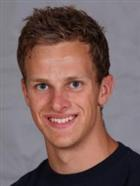
\includegraphics[scale=0.55]{figs/mads.jpeg} \\
	Mads Friis Bornebusch (s123627)\\ [10pt]
		\vspace{0.15cm}
	\end{center}
	\end{minipage}
\end{figure}

\begin{figure}[h!]
	\centering
	\begin{minipage}{0.40\linewidth}
	\begin{center}
	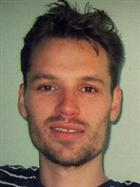
\includegraphics[scale=0.55]{figs/tobias.png} \\
	Tobias Tuxen (s120213)\\[10pt]
		\vspace{0.15cm}
	\end{center}
	\end{minipage}
\end{figure}

\begin{figure}[h!]
	\centering
	\begin{minipage}{0.40\linewidth}
	\begin{center}
	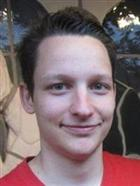
\includegraphics[scale=0.55]{figs/kristian.jpeg} \\
    Kristian Sloth Lauszus (s123808) \\ [10pt]
		\vspace{0.15cm}
	\end{center}
	\end{minipage}
\end{figure}


\vspace*{\stretch{2}}
\end{center}
\begin{flushleft}
\subtitle\\
DTU Space\\
\dato
\end{flushleft}


	
	%%% INDHOLDSFORTEGNELSE OG ABSTRACT %%%
		\chapter{Abstract}

In this programming project we have written and designed all the code to the game Reflex Ball. The code has been written in C in the compiler Z8Encore! and has been implemented on a Zilog 6403 Mircrocontroller. \\ \\
We have concluded that the written code implements the desired circuit on the Microcontroller as as all the different facilities of the game has been thoroughly tested and is in compliance with the expected result. In the end we have a fully functional Reflex Ball Game with many expansions, which amongst others, include bricks (Arkanoid style), power-ups, different levels and steering-wheel game controller. So far no bugs has been found in the final version of the game.

\begin{figure}[h!]
\centering
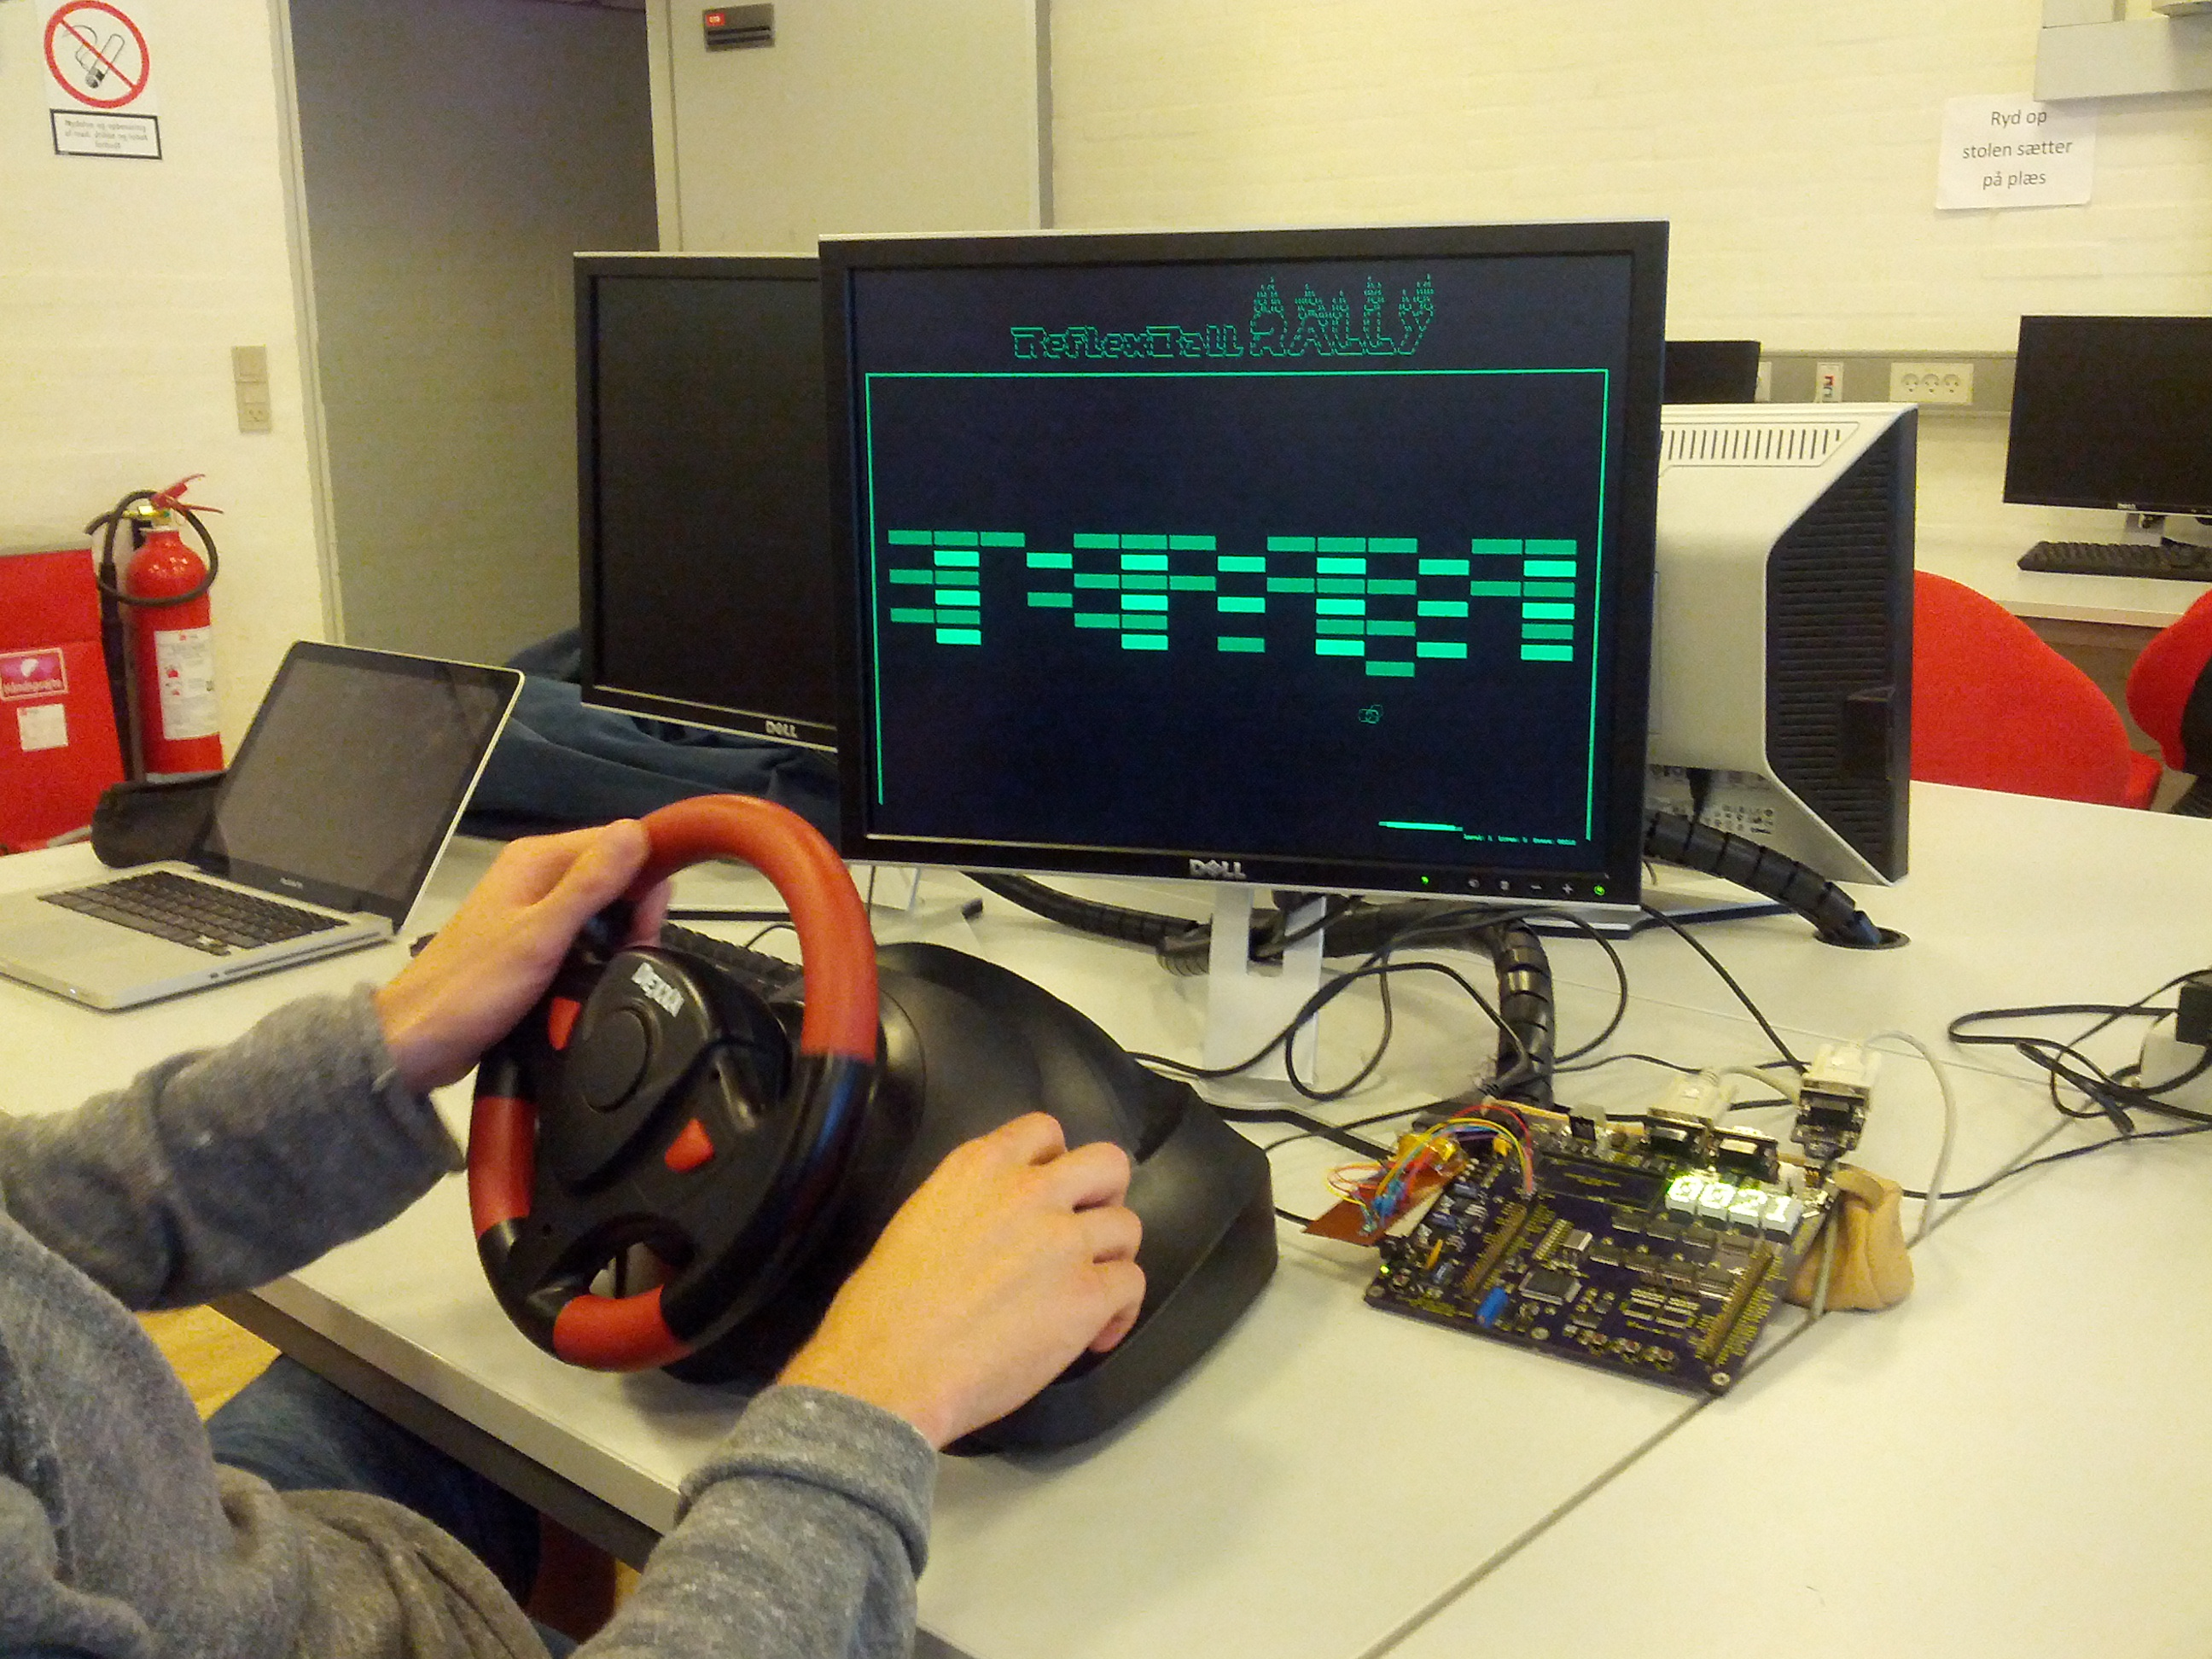
\includegraphics[scale=0.5]{figs/forside.png}
\caption{Screenshot from our implementation of ReflexBall}
\label{fig:awesome}
\end{figure}
		\chapter{Resumé}

I dette programmeringsprojekt har vi skrevet og designet al koden til spillet Reflex Ball. Koden er skrevet i C i compileren Z8Encore! og implementeret på en Zilog 6403 mircocontroller. \\ \\
Vi har konkluderet at den skrevne kode implementerer det ønskede kredsløb på Mircrocontrolleren, da alle spillets facetter er blevet gennemtestet og giver det ønskede output. Som slutresultat har vi et fuldt funktionelt ReflexBall-spil med mange udvidelser der bl.a. inkluderer brikker (Arkanoid-stil), power-ups, forskellige levels og styring med ret. Der er indtil videre ikke fundet nogle bugs i slutversionen af spillet.\\ \\
		\newpage
		\chapter{Fordord}

Denne rapport er skrevet som en del af eksaminationen i DTU kursus 30010 Programmeringsprojekt. Alle tre, på forsiden nævnte, gruppemedlemmer har bidraget til rapporten på lige vis. Vi har lavet alle forberedelsesøvelser, skrevet koden og afsnittene i rapporten i fællesskab. Denne rapport beskriver vores arbejde og resultater.\\ \\ \\ \\ \\ \\

\begin{figure}[h!]
\centering
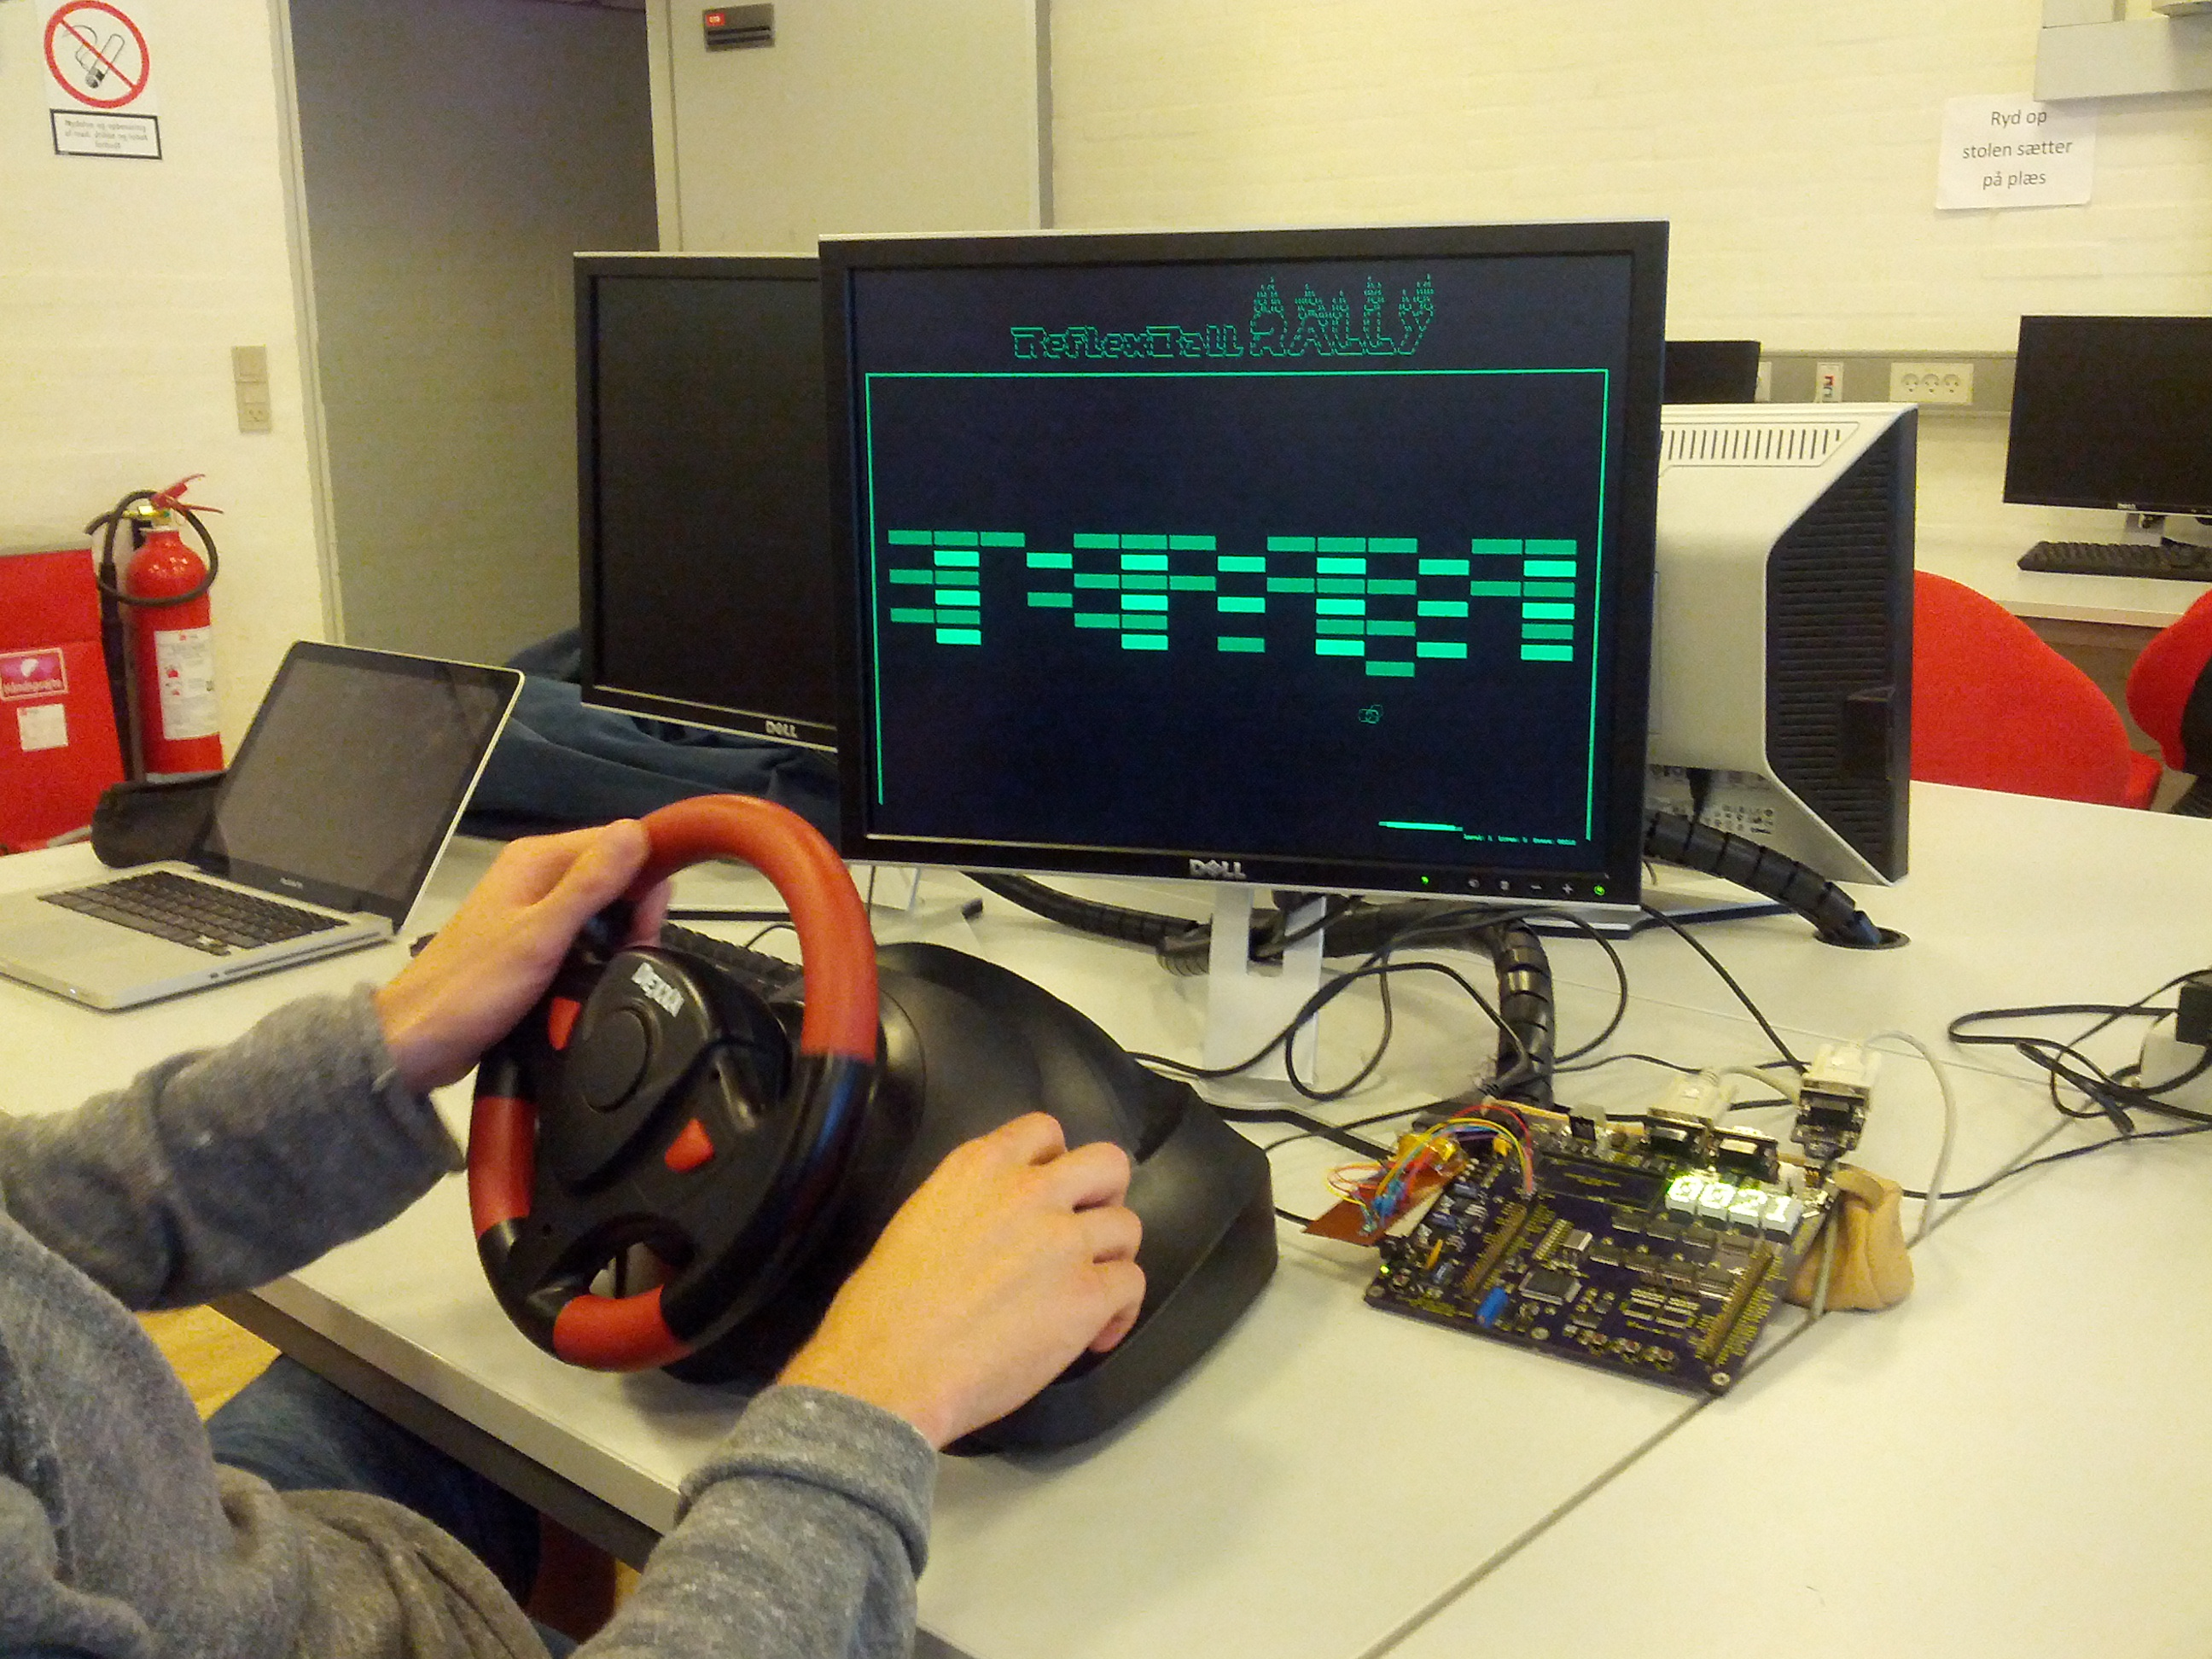
\includegraphics[scale=0.17]{figs/forside.jpg}
\caption{Screenshot from our implementation of ReflexBall}
\label{fig:forside}
\end{figure}
		\newpage
		\tableofcontents*						% Indholdsfortegnelse (fjern * hvis der skal stå "Indhold")
%        \listoffigures*						% Figurliste

		
	%%% RAPPORTINDHOLD %%%
		\mainmatter
%		\input{tex/maple}
		\chapter{Introduktion}
Denne rapport dokumenterer de overvejelser vi har gjort os i forhold til design og struktur af Reflex Ball spillet. \\
Programmeringsprojektet har overordnet set været inddelt i to faser.\\

Første del, der inkluderede de fire første arbejdsdage, blev brugt på at lave håndregningsøvelser omhandlende manipulation af hexadecimal- og bitrepresenterede tal og flere programmerings-øvelser i C, også omhandlende hexadecimal- og bitmanipulation samt ansi-koder, driverhåndtering og vektorregning og styring a LED-display. Formålet med disse øvelser var samlet set at blive bedre til at håndtere hexadecimal- og bitrepresenterede tal, og desuden at lære om/genopfriske pointers, headers og opsætning af hardware-drivere til microcontrolleren.\\

Anden del af projektet, der inkluderede de sidste ni arbejdsdage, har vi brugt på først at designe Reflex Ball-spillet ud fra de i opgaven specificerede krav og derefter implementere udvidelser både på hardware- og softwareniveau, sideløbende med vi hele tiden har videreudviklet spillets 'engine', så spillet bruger mindre RAM og kører så fejlfrit som muligt, samtidig med at koden gradvis er blevet gjort mere fleksibel og overskuelig.\\

		\chapter{Specifikationer}

Nedenfor er vores forskellige delmål i projektet. Spillet skal have de nedenstående funktionaliteter. Listen kan derfor ses som kravene til hvad vores spil skal kunne og er samtidig opdelt på en logisk måde så man kan starte fra toppen af og arbejde sig igennem delmålene indtil man har et færdigt spil der fungerer og ser ud efter vores hensigt. Delmålene er samtidig bygget op på en sådan måde, at skulle der ikke være tid til at nå det hele, har man stadigvæk et fuldt funktionelt spil. Det vil altså sige at vi arbejder fra basale funktionaliteter ud mod mere specifikke og detaljerede elementer.\\

\textbf{Delmål Basics}
\begin{itemize}
\item Detektere tastatur-input så keyboardet kan bruges til at styre striker
\item Tegne banen
\item Bevæge strikeren
\item Bevægelig bold
\item Bolden reflekteres af striker, loft og vægge
\item Det skal detekteres når bolden er under strikeren (man er død)
\end{itemize}

\textbf{Delmål advanced}
\begin{itemize}
\item Liv-system, så man har 3 liv inden man bliver Game Over
\item Pointsystem
\item Ændring i boldhastighed som ens score stiger
\item Internt 18.14 koordinatsystem, så boldens bevægelse kan laves som en enhedsvektor der kan roteres rundt
\item Bolden skal starte i en tilfældig vinkel
\item Striker-zoner, så boldens afbøjningsvinkel afhænger af hvor den rammes 
\item Stor bold, der fylder 4x2 monospace-karakterer.
\item {Forskellige sværhedsgrader}
\item {Brikker og forskellige baner}
\end{itemize}
	

\textbf{Brikker}
\begin{itemize}
\item Banen skal indeholde brikker
\item Der skal være forskellige typer af brikker (forskellig antal liv)
\item Der skal være forskellige levels med brikker i forskellige mønstre
\item Når bolden rammer brikker og kanter skal den reflekteres på en logisk måde så fysikken i spillet ser realistisk ud
\end{itemize}

\textbf{Helhedsindtryk}
\begin{itemize}
\item LED display med score, liv og levels
\item Menu hvor man kan vælge sværhedsgrad
\item Beskeder ved Game Over
\item Besked hvis spillet vindes
\item Implementering af ASCII-Art tekst og billeder til Menu, Game Over og Win
\end{itemize}

\textbf{Hardware}
\begin{itemize}
\item Styring med intern hardware (knapper på microcontrolleren)
\item Tilslutning af ekstern hardware (DEXXA Steering Wheel)
\end{itemize}

Vi har lagt en del vægt på at spillet skal se realistisk ud og at bolden, strikeren og brikkerne skal flytte sig på en realistisk måde. Vi vil forsøge at lave spillets fysik så dette er opfyldt, så bolden bevæger sig så naturligt og logisk som muligt. 

		\chapter{Tidsplan}
Fra starten af lagde vi en plan over hvornår vi ville udføre de delmål vi havde. Denne plan fremgår af figur \ref{fig:tidsplan1}. Som det kan ses var planen at starte med basic-delmålene og derfra bevæge os ud mod de mere avancerede som liv, hastighed, score, internt koordinatsystem, sværhedsgrader osv. Efterfølgende ville vi implementere et DEXXA Steering Wheel som controller til sjovere styring af spillet.\\
Efter dette ville vi begynde på hvad man kan kalde en finpudsning af spillet, dvs. ordentlig start menu og beskeder hvis spillet vindes eller tabes. \\

Efterfølgende ville vi lave achievements, altså power-up's og power-down's til spillet. Vi fandt lynhurtigt masse potentielle af disse, såsom at strikeren skulle kunne blive bredere/smallere, bolden skulle kunne klistre til strikeren, bolden skulle kunne skydes direkte igennem brikkerne uden at blive reflekteret og størrelsen og hastigheden af bolden skulle kunne ændres osv. Vi havde rent faktisk så mange idéer, at kun tiden satte grænser for hvor mange achievements vi ville implementere. Vi valgte at sætte dette som det tredje sidste punkt i planen, da achievements skulle være en bonus til en allerede spilbart og udfordrende gameplay.\\ \\


\begin{figure}[h!]
\centering
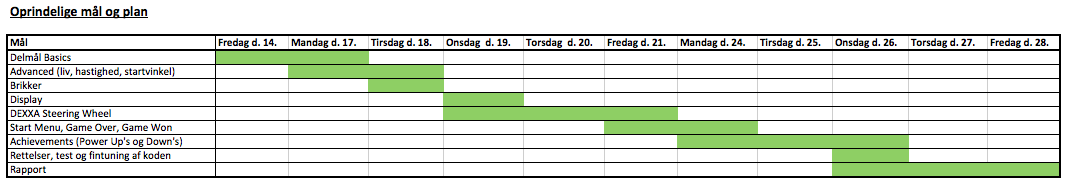
\includegraphics[width=\textwidth]{figs/Tidsplan1.png}
\caption{Tidsplan over de forskellige delmål og hvornår de skulle være færdige}
\label{fig:tidsplan1}
\end{figure}
		\chapter{Struktur}

\section{Basics}
Da vi skulle planlægge projektet valgte vi efter en brainstorm at dele projektet op i en mængde delmål vi ville have implementeret. Delmålene i kategorien basics var dem vi skulle implementere for at have et fungerende spil. Vi fandt frem til at det skulle være følgende funktionaliteter.\\

\underline{Keyboard input}\\

Vi har valgt at man i basic implementeringen af spillet laver al styring vha. keyboardet, da knapperne på udviklings boardet var al for slidte og derfor virkede dårligt. Vi implementerede det sådan så man bevæger strikeren ved hjælp af piletasterne på tasteturet og sender bolden af sted ved space-tasten. Hvis man dør og bliver Game Over startes spillet forfra ved tryk på space-tasten. Der er dog et 1000ms delay fra man dør til spillet kan startes forfra. På den måde kommer man ikke til at starte spillet forfra uden at opdage at man døde.\\
\newpage

\underline{Banen}\\

Banen har vi implementeret i et koordinatsystem på den måde at vi har  x$_{1}$- og x$_{2}$-koordinater, svarende til banens bredde (x$_{1}$ = banens venstre væg, x$_{2}$ = banens højre væg) og y$_{1}$- og y$_{2}$-koordinater, svarende til banens højde (y$_{1}$ = loft, y$_{2}$ = 'gulv'). Vi arbejder i vores implementering med et venstredrejet koordinatsystem, hvor y-aksen er inverteret i forhold til et almindeligt koordinatsystem, så y$_{2}$ har altid en større værdi end y$_{1}$.\\

\underline{Udnyttelse af Timer}\\

Da vi ofte har brug for at kunne bestemme tiden siden sidste gang en bestemt funktion blev kaldt, opsatte vi Timer1 til at interrupte hvert 1ms. I dette interrupt forøgede vi en variable \texttt{mscounter}. Denne er således et udtryk for hvor lang tid siden der er gået siden programmets start i millisekunder. Ved at kalde funktionen \texttt{millis()} der returner \texttt{mscounter} kunne vi således let bestemme hvad hvor langt tid der var gået siden sidst funktionen blev kaldt hvis vi havde gemt denne tid i en variable.\\

\underline{Bevægelig striker}\\

Til strikeren har vi lavet et \texttt{struct}, der er givet ved strikerens x-værdi (yderstre venstre karakter af strikeren), y-værdi, samt sin bredde.
Strikeren er blevet implementeret på den måde at når den rykkes til venstre, tjekkes der om strikerens x-værdi, minus det antal felter den skal rykkes til venstre, er mindre end eller lig med banens venstre side (dvs. banens x$_{1}$-værdi). Hvis dette er tilfældet befinder strikens sig ved dens venstre yderposition og sættes dermed til at være helt ude til venstre med venstre siden mod væggen.
Hvis strikeren er ude i sin yderste venstre position er strikerens x-værdi nemlig 1 større end banens x$_{1}$-værdi, strikeren x-værdi må således aldrig blive lig eller mindre end banens x$_{1}$-værdi, da den således ville befinde sig uden for banens vægge. \\

Hvis strikerens x-værdi derimod er større end banens x$_{1}$-værdi, trækkes der det antal felter den skal rykkes fra strikerens x-værdi. Derefter fjernes de felter strikeren har rykket væk fra og strikeren tegnes på ny. \\

Når strikeren bevæger sig til højre fungerer samme princip, bare hvor der tjekkes om \texttt{striker.x + striker.width-1+antal\_ryk} er større eller lig med banens x$_{2}$-værdi. 

Hvis testen er positiv sker ingenting og strikeren bliver stående, hvis testen er negativ overskrives felterne det antal felter den skal rykke med mellemrum i venstre side. Derefter tegnes strikeren igen. \\

I denne første implementation af spillet blev strikeren bygget til først at rykke sig et monospace ad gangen, derefter satte vi det op til at strikeren bevægede sig to monopaces ad gangen. Dette var vi nødt til at gøre eftersom vi styrede strikeren med keyboardet og der i keyboardets hardware er en lavere grænse for maksimumsfrekvensen hvormed en knap bliver genaktiveret når knappen på keyboardet holdes nede, i forhold til microcontrolleren der har en højere maksimumsfrekvens. Her i Basics-implementationen byggede vi banen sådan så det passede med at strikeren altid kun rykkede to felter ad gangen indtil den kom ud i banens yderpositioner.\\
\newpage

\underline{Bevægelig bold}\\

Ved at aflæse timer funktionen \texttt{millis()} hver gang vi kalder funktionen \texttt{updateGame()}, kan vi bestemme hvor lang tid der er gået siden sidste gang vi opdaterede spillet. Hvis der således er gået længere end en bestemt værdi bevægede vi bolden og opdaterede resten af spil-logikken.\\

Her i basics implementationen hardcodede vi dette til at boldens x-værdi ændrede sig med plus 1 for hvert tick og boldens y-værdi ændrede sig med minus 1 for hvert tick, når bolden blev skudt afsted fra strikeren. Dette skyldes at vi jo arbejder med en inverteret y-akse i forhold til et almindeligt koordinatsystem. Det fungerer på den må at vi har et \texttt{Ball struct} sådan så bolden hele tiden kender sin egen position i form af x- og y-koordinat, samt en vektor (den retning og hastighed den bevæger sig i). Så når bolden rykker sig, overskrives feltet som er boldens (x,y)-koordinat med et mellemrum (da bolden i basic implementationen kun fylder et enkelt felt) og derefter tillægges boldens vektor til boldens (x,y)-koordinat og den gentegnes.\\

\underline{Reflex-logik på kanter og hjørner}\\

Hver gang bolden har rykket sig, inden den tegnes, laves en række tjek for at se om bolden har ramt en væg, et hjørne eller loftet. Bl.a. tjekkes om boldens x-koordinat bliver større end eller lig med banens x$_{2}$-koordinat. Hvis dette er tilfældet ved vi at bolden har ramt højre væg af banen og bolden tegnes ikke umiddelbart. Det der i stedet for skal ske er at boldens vektor skal trækkes fra boldens nye (x,y)-koordinat, sådan så bolden er tilbage på den plads den stod på inden den ramte ind i væggen, derefter skal boldens vektors x-komposant inverteres og vektoren skal lægges til boldens position inden bolden igen bliver tegnet på næste tick. Det var netop sådan vi implementerede kant-logikken til at starte med. Efterfølgende ændrede vi dette til at at hvis bolden rammer højre væg, så trækkes 2 fra boldens x-koordinat og boldens vektors x-komposant inverteres. Effekten af de to implementeringer er den samme, forskellen er bare at den sidste kræver lidt færre beregninger og den er derfor mere effektiv.\\
Når bolden rammer venstre væg fungerer der på præcis samme måde, bortset fra at tjekket er om boldens x-koordinat bliver mindre eller lig med banens x$_{1}$-koordinat og hvis dette er tilfældet inverteres vektorens x-komposant og der ligges 2 til boldens x-koordinat.\\

Loftet fungerer også mere elle mindre på samme måde. Her tjekkes bare om boldens y-koordinat kommer under banens y$_{1}$-koordinat (husk y-aksen er inverteret). Hvis dette er tilfældet inverteres vektorens y-komposant og der ligges to til boldens y-koordinat inden den tegnes igen. \\

Al refleks-logikken tjekkes med if-sætninger, sådan så hver gang bolden har bevæget sig tjekkes først om den har ramt banens højre side, derefter banens venstre side og derefter loftet, inden den gentegnes. Så hvis fx bolden rammer højre øvre hjørne sker der det at refleks-logikken først detekterer at banens højre side er overskredet og derfor inverteres vektorens x-komposant og boldens x-koordinat formindskes med 2. Efterfølgende detekteres at bolden har ramt loftet og derfor tillægges to til boldens y-koordinat, samtidig med at vektorens y-komposant inverteres. Når bolden tegnes igen er den tilbage på feltet den var på 2 gange forinden den ramte væggen, med både x- og y-komposant af vektoren inverteret, hvilket er det ønskede resultat.\\

\underline{Game Start og Game Over}\\

Når spillet starter kan man rykke strikeren rundt som normalt. Her følger bolden med sådan så den bliver ved med at være på midten af strikeren. Det fungerer på den måde at når variablen \texttt{gameStarted} er 0 så gentegnes både strikeren og bolden hver gang man rykker strikeren. Både boldens og strikerens x-koordinat sættes herefter. På samme måde som når strikeren rykkes normalt laves de samme check for om strikeren har bevæget sig ud over banens vægge. Når der så trykkes på space-tasten på tasteturet skydes bolden afsted og \texttt{gameStarted} sættes til 1, og når strikeren nu rykkes er det kun strikeren der gentegnes.\\

På samme måde som bolden hver gang den har bevæget sig, inden den tegnes, testes for om den har ramt vægge eller loft, tjekkes også om boldens y-koordinat lig strikerens y$_{2}$-koordinat. Hvis denne test er sand betyder det at bolden ligger på feltet lige i strikeren. Her testes så om boldens x-koordinat ligger indenfor strikeren, dvs. imellem \texttt{striker.x} og \texttt{striker.x + striker.width}. Hvis dette er tilfældet bliver bolden skudt op igen, hvilket fungerer ved at boldens vektors y-komposant bliver inverteret, på samme måde som når bolden rammer loftet. Hvis bolden er uden for strikeren bliver variablen \texttt{alive} sat til 0 og der vises \texttt{Game Over!} midt på skærmen. I denne tilstand kan man ikke bevæge strikeren. Dette har vi implementeret fordi man ellers kan 'køre bolden over', da bolden jo ligger nede på gulvet, hvilket ikke ser så grafisk pænt ud. Når der trykkes space igen gentegnes hele spillet banen og og variablerne \texttt{gameStarted} sættes til 0 og \texttt{alive} sættes til 1.

\section{Advanced}
Efter alle basics var færdig-implementeret, havde vi planlagt at lave en række udvidelser til spillet. Disse omfatter dels implementering af liv og pointsystem, men også videreudviklinger af basic-funktionaliteterne, sådan så deres bagvedliggende virkemåde gøres mere avanceret. Advanced inkluderer følgende.\\

\underline{Liv}\\

Som i ethvert andet arkade-spil har vi implementeret liv, sådan så man starter med tre og bliver Game Over, når der er nul liv tilbage. Som en ekstra feature har vi implementeret at man får 2 ekstra liv, når en bane er gennemført.\\

\underline{Pointsystem}\\

Scoren er opbygget sådan så det giver 1 point hver gang man rammer en brik. Vi har valgt at det ikke skal give nogle point når bolden rammer strikeren, da vi ikke synes det skal give point 'ikke' at ramme brikkerne.\\

\underline{Internt 18.14 koordinat-system}\\

I basic-implementeringen af spillet satte vi bolden til at rykke sig et bestem antal monospaces hver gang den bevægede sig, altså en simpel vektor-implementering. Men efter denne udvidelse er hele banens indre struktur blevet gentænkt sådan så bolden bevæger sig som en enhedsvektor i et internt koordinatsystem. Som nævnt i basics har vi lavet et \texttt{Ball struct} sådan så bolden hele tiden kender sine egne (x,y)-koordinater, samt nu dens egen enhedsvektor (altså retning hvori den bevæger sig). I denne udvidelse valgte vi dog at angive disse værdier i et 18.14 format, så vi får en meget højere opløsning for boldens bane. \\
Når bolden bevæger sig sker der det at dens vektors (x,y)-koordinat lægges til boldens (x,y)-koordinat. Derefter tjekkes om bolden er død eller har ramt en brik, en væg, et hjørne, strikeren eller loftet. Hvis intet af dette er tilfældet, slettes boldens gamle koordinater ved at der på disse felter tegnes blanke mellemrum. Derefter afrundes boldens (x,y)-koordinater til nærmeste heltal ved at kigge på 1. bit efter kommaet, det vil sige boldens x- hhv. y-koordinats 13. bit (da det tænkte komma er sat mellem 14. og 13. bit). Hvis denne er 0 rundes ned og ellers rundes op. Nu kendes boldens (x,y)-koordinat i heltal og den kan derfor indtegnes på banen.\\

\underline{Vilkårlig startvinkel}\\

Når bolden skydes af bliver den sendt afsted i en vilkårlig vinkel på mellem 45 og 135 grader. Det vil sige lodret op fra strikeren plus minus op til 45 grader. Dette er implementeret for at man ikke kan time startvinklen så man er sikker på den altid rammer et bestemt sted.\\

\underline{Striker-zoner}\\

Strikeren er opbygget sådan så den altid skal bestå af et lige antal felter. Dens midterste venstre felt har en afbøjningsvinkel på indgangsvinkel plus 0 grader, og dens yderste venstre felt har en afbøjningsvinkel på indgangsvinkel plus ca. 45 grader. Hvert felt mellem det midterste venstre til det yderste venstre felt, har så en stigende afbøjningsvinkel, hvor den vinkel der bliver lagt til hvert felt er 45 grader divideret med antallet af felter fra det midterste venstre (eksklusiv) til det yderste venstre (eksklusiv). Højre-siden af strikeren fungerer på præcis samme måde, bare med omvendt fortegn, sådan så afbøjningsvinklen på midterste højre felt er lig indgangsvinklen og afbøjningsvinklen på yderste højre felt er lig indgangsvinklen minus 45 grader.\\
Alt dette er lavet ved at boldens reflekslogik er gentænkt sådan så dens vektors x- og y-komposant nu bare  er lig vektorens sinus hhv. cosinus-værdi, da boldens vektor nu hele tiden er en enhedsvektor. Når bolden skal reflekteres kan vi så bruge  den sinus look-up table, som vi fik givet som led i en af introduktionsopgaverne.\\

Strikeren er lavet på denne måde så dens bredde er meget fleksibel. Fx bruges der forskellige striker-størrelser på spillets forskellige sværhedsgrader og dette er så bare implementeret ved at ændre på størrelsen af \texttt{striker.width}. Så sørger spillet selv for at inddele Striker-zonerne. \\

Figur \ref{fig:striker_zones} viser hvordan strikeren er opdelt i zoner for en striker med længden 10 og en bold med længden 4. Det ses hvis bare boldens ene ende er inde over midten, så afbøjes den ikke. Hvis bolden derimod kun rører med den ene kant, så afbøjes den med den maksimale vinkel $\pm$ 42.2 grader.

\begin{figure}[h!]
\centering
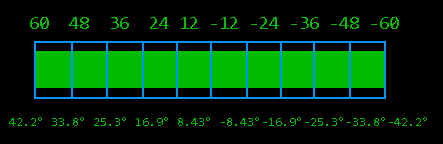
\includegraphics[scale=0.8]{figs/striker_zones.png}
\caption{Oversigt over striker zoner for en striker der er med længden 10 og en bold med længden 4}
\label{fig:striker_zones}
\end{figure}
\newpage

Der er desuden implementeret en minimums-afbøjningsvinkel på 15 grader og en maksimums-afbøjningsvinkel på 165 grader. På samme måde som når bolden rammer noget andet, bitshiftes boldens vektors x-komposant 1 til højre når bolden rammer strikeren, sådan så boldens vektor igen er en enhedsvektor. Derefter beregnes boldens afbøjningsvinkel. Hvis dennes y-værdi er mindre end 0,25, svarende til sinus til ca. 15/165 grader, ved vi at boldens vinkel er enten under 15 grader eller over 165 grader efter afbøjning og afbøjningsvinklen bliver derfor sat til 15 grader hvis \texttt{ball.vector.x} er positiv og til 165 grader hvis \texttt{ball.vector.x} er negativ.\\

\underline{Stor bold}\\

I \texttt{Ball struct} er der ud over x- og y-koordinater og en vektor to andre variable som er bredde (\texttt{width}), højde (\texttt{height}). Den bold vi bruger i spillet har en højde på 2 og en bredde på 4. Dette komplicerer en del ting eftersom bolden nu både kan rammer alle objekter (striker, vægge, loft, brikker) på mange flere måder. Desuden er der en grænse for hvor hurtigt uarten kan arbejde, selvom vi har sat baud-raten op til maksimum (115200), dette kan godt gå hen og blive lidt problematisk, da uarten ved en vis hastighed af bolden ikke kan nå at slette og gentegne den ordentligt. Som løsning på dette, har vi sørget for at bolden ved en vis hastighed kun tegnes hver anden gang, hvilket letter UART'ens arbejde en smule. Læs mere om dette under  afsnittet om \texttt{Rettelser og fintuning}.\\

\underline{Sværhedsgrader og ændring i boldens hastighed}\\

I spillet er der implementeret fire forskellige sværhedsgrader. Disse er Easy, Medium, Hard og Chuck Norris. Forskellen på sværhedsgraderne er hvor bred strikeren er, hvor hurtig starthastighed bolden har og hvor mange point man skal have før at boldens hastighed bliver sat op. På Easy er \texttt{striker.width} = 30 og boldens starthastighed er 40ms. Det vil sige der går 40ms fra bolden bliver tegnet, til den tegnes igen. På Medium er \texttt{striker.width} = 20 og boldens starthastighed 40ms, på Hard er \texttt{striker.width} = 10 og boldens starthastighed 40ms og på Chuck Norris er \texttt{striker.width} = 4 og boldens starthastighed er 10ms.\\

Som man får flere point sættes boldens hastighed op. På Easy bliver delayet mellem to på hinanden følgende gange hvor bolden tegnes, sat 1ms ned for hvert 10 point man får. På Medium ved hvert 5. point man får og på Hard ved hvert 2. point man får. Når delayet mellem bold-aftegningerne kommer under 20 ms begynder bolden kun at blive tegnet hver anden gang for at UART'en kan følge med. Minimumshastigheden som bolden kan bevæge sig i er 10ms delay mellem aftegningerne. Grænsen er sat her fordi spillet ellers bliver for umuligt at gennemføre. Da Chuck Norris-sværhedsgraden starter på 10ms delay øges boldhastigheden altså ikke uanset hvor mange point man får.\\
Når der skiftes bane bliver boldhastigheden resat til starthastigheden ved den givne sværhedsgrad. Dvs. 40ms delay på Easy, Medium og Hard og 10ms på Chuck Norris.\\

\underline{Brikker og baner}\\

Som en del af de avancerede mål havde vi at lave brikker, så gameplayet bliver sjovere. Se mere om implementering af brikker, forskellige brik-typer og forskellige baner i afsnit \textbf{3.3}.\\ \\ \\ \\


\section{Brikker}

Formålet med at implementere brikker i spillet var at give gameplayet en helt ny dimension.\\

\underline{Tegne Brikker.}\\

For lettest at kunne holde styr på brikkerne har vi lavet en struct, \texttt{Brick} der repræsenterer en brik. Den indeholder position i x- og y-koordinater, bredde, højde og brikkens liv. Brikkerne i en bane er gemt i et array:\\ \texttt{Brick bricks[BRICK\_TABLE\_HEIGHT][BRICK\_TABLE\_WIDTH]}. Når banen initialiseres gennemløbes dette array og hver brik tildeles koordinater, bredde, højde og liv. Efter dette tegnes brikken. Hvis brikken har 0 liv svarer det til at der ikke er en brik. Ved at give brikkerne i array'et forskellige antal liv kan man lave mønstre med brikkerne så man på den måde har flere forskellige baner i spillet. På Figur \ref{fig:brikker} er der vist hvordan brikker med forskelligt antal liv er tegnet. Jo flere liv de har, des mere solide tegnes de. Som et lille twist i gameplayet har vi valgt at gøre brikker med mere end fire liv usynlige så de pludseligt kan dukke op når man rammer dem. 
\newpage

\begin{figure}[h!]
\centering
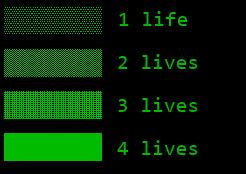
\includegraphics[scale=1]{figs/brikker.png}
\caption{Brikker med forskelligt antal liv tegnes forskelligt}
\label{fig:brikker}
\end{figure}


\underline{Baner gemt i et array i ROM'en.}\\

Vi har valgt at hardcode brikkernes bredde og højde for at spare plads når vi gemmer banerne i ROM'en. På denne måde kan en bane i ROM'en gemmes i arrayet\\ \texttt{unsigned char rom levels[6][BRICK\_TABLE\_HEIGHT][BRICK\_TABLE\_WIDTH]}. Dette arrray er et tredimensionalt array af chars der er gemt i ROM'en. Det indeholder 6 "lag" der hver indeholder de todimensionale data til en bane. Værdien af hver char er antallet af liv den tilsvarende brik får. Når banen initialiseres, løbes dette array og arrayet\\ \texttt{bricks[BRICK\_TABLE\_HEIGHT][BRICK\_TABLE\_WIDTH]} igennem og brikkerne i \texttt{bricks} får det antal liv der står i \texttt{levels} arrayet. Den dynamiske hukommelse i mikroprocessoren indeholder således kun et array af brikker der svarer til den aktuelle bane. Et eksempel på hvordan en bane er gemt i arrayet \texttt{levels} er vist nedenfor.

\begin{lstlisting}
{ 
	{ 0, 0, 0, 0, 0, 0, 0, 0, 0, 0, 0, 0, 0, 0 },
	{ 0, 0, 0, 0, 0, 0, 0, 0, 0, 0, 0, 0, 0, 0 },
	{ 0, 0, 0, 0, 0, 0, 0, 0, 0, 0, 0, 0, 0, 0 },
	{ 0, 0, 0, 0, 0, 0, 0, 0, 0, 0, 0, 0, 0, 0 },
	{ 0, 0, 0, 0, 0, 0, 0, 0, 0, 0, 0, 0, 0, 0 },
	{ 0, 0, 0, 0, 0, 0, 0, 0, 0, 0, 0, 0, 0, 0 },
	{ 0, 0, 0, 0, 0, 0, 0, 0, 0, 0, 0, 0, 0, 0 },
	{ 1, 1, 1, 0, 1, 1, 1, 0, 1, 1, 1, 0, 1, 1 },
	{ 0, 3, 0, 2, 0, 3, 0, 2, 0, 3, 0, 2, 0, 3 },
	{ 1, 1, 1, 0, 1, 1, 1, 0, 1, 1, 1, 0, 1, 1 },
	{ 0, 3, 0, 2, 0, 3, 0, 2, 0, 3, 0, 2, 0, 3 },		
	{ 1, 1, 1, 0, 1, 1, 1, 0, 1, 1, 1, 0, 1, 1 },
	{ 0, 3, 0, 2, 0, 3, 0, 2, 0, 3, 0, 2, 0, 3 },
	{ 1, 1, 1, 0, 1, 1, 1, 0, 1, 1, 1, 0, 1, 1 },		
	{ 0, 0, 0, 0, 0, 0, 0, 0, 0, 0, 0, 0, 0, 0 },
	{ 0, 0, 0, 0, 0, 0, 0, 0, 0, 0, 0, 0, 0, 0 },
	{ 0, 0, 0, 0, 0, 0, 0, 0, 0, 0, 0, 0, 0, 0 },
	{ 0, 0, 0, 0, 0, 0, 0, 0, 0, 0, 0, 0, 0, 0 },
	{ 0, 0, 0, 0, 0, 0, 0, 0, 0, 0, 0, 0, 0, 0 },
	{ 0, 0, 0, 0, 0, 0, 0, 0, 0, 0, 0, 0, 0, 0 },
},
\end{lstlisting}
Banen der svarer til det ovenstående array, er vist på Figur \ref{fig:level1}. 

\begin{figure}[h!]
\centering
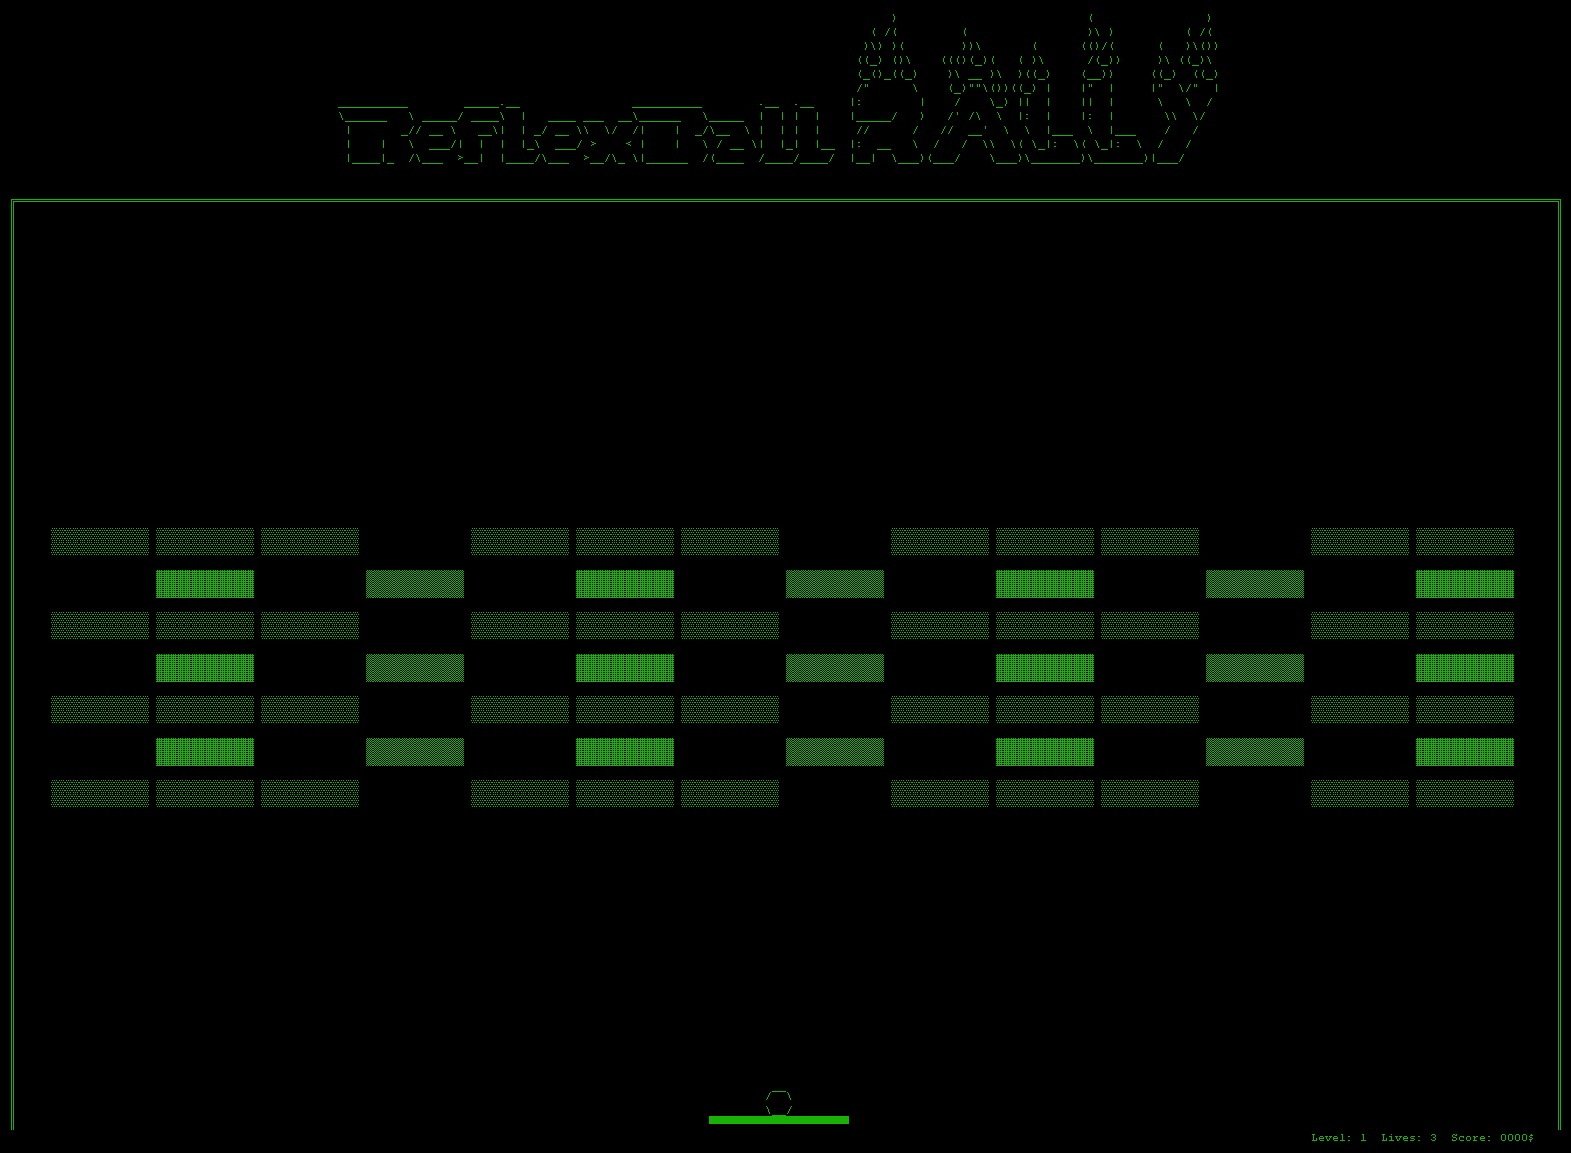
\includegraphics[scale=0.25]{figs/screenshots/level1.png}
\caption{Level 1 i spillet}
\label{fig:level1}
\end{figure}

\newpage

\underline{Tjekke om man rammer brikker.}\\

Den helt store udfordring med brikkerne var at tjekke om bolden ramte dem. Ved hver eneste iteration af spillet gennemløber vi arrayet \texttt{bricks[][]} og for alle brikker med mere end 0 liv tjekker vi om bolden har ramt og i givet fald hvordan.\\
Når spillet itereres og bolden flyttes tjekker vi først om bolden rammer brikkerne før vi tegner den. Hvis bolden har ramt en brik reflekteres den og får sin nye position før den tegnes. Hvis bolden har ramt en brik, er boldens koordinater altså inde i brikken når vi tjekker.\\

For at bolden skulle bevæge sig lige hurtigt i begge retninger på skærmen har vi lavet x-komposanten af boldens vektor dobbelt så stor, da der var næsten præcis dobbelt så stor opløsning i x-aksen i forhold til y-aksen. Det giver nogle ekstra udfordringer når bolden rammer brikkerne. Når bolden kan bevæge sig 2 karakterer i x-retningen kan den ramme brikkerne fra siden på en række forskellige måder. Disse er vist for højre side af brikken på Figur \ref{fig:SideReflexSamlet}. 
Når vi har itereret spillet og tjekker boldens position kan den på x-aksen befinde sig både en eller to karakterer inde i brikken. Den kan således ramme brikken på seks forskellige måder som vist på ovennævnte figur. Det er vigtigt at tage højde for at bolden kan ramme to karakterer ind i brikken, når man tjekker om bolden har ramt brikken midtpå fra siden. Hvis man ikke tager højde for dette, vil bolden bevæge sig igennem brikken mens den reflekteres af toppe og bunden.\\

\begin{figure}[h!]
\centering
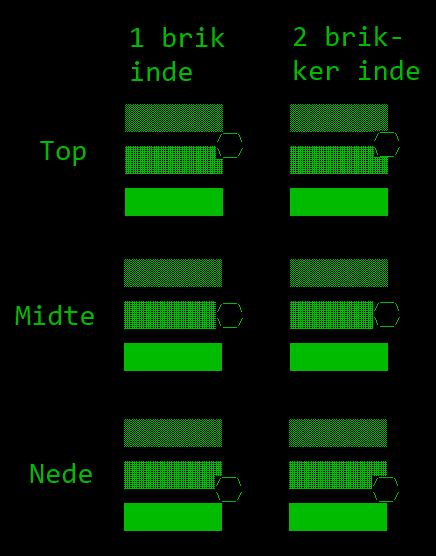
\includegraphics[scale=0.75]{figs/side_reflex_samlet.png}
\caption{Forskellige måder bolden kan ramme fra siden}
\label{fig:SideReflexSamlet}
\end{figure}
\newpage

For at give et godt gameplay har vi besluttet at bolden fortrinsvis skal reflekteres op og ned så brugeren kan få den. Dette er vist på Figur \ref{fig:ReflexOppeFri}. Når bolden rammer brikken fra toppen og er 2 karakterer inde i brikken vil den blive reflekteret som vist på figuren. Hvis bolden havde ramt på samme måde, men var kommet nedefra var den blevet reflekteret som om den havde ramt siden af brikken.\\

Det der er vist på denne figur er, borset fra de omgivende brikker, samme situation som på Figur \ref{fig:SideReflexSamlet}, Top, 2 brikker inde. 
\begin{figure}[h!]
\centering
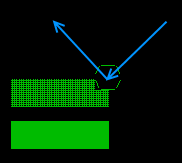
\includegraphics[scale=1]{figs/reflex_oppe_fri.png}
\caption{Forskellige måder bolden kan ramme fra siden}
\label{fig:ReflexOppeFri}
\end{figure}

\underline{Hjørnerne.}\\

Et specialtilfælde er når en brik bliver ramt lige på hjørnet, en karakter inde. Her er tre mulige situationer som vist på Figur \ref{fig:cornerReflex}. Den eneste forskel på de tre tilfælde er hvor de omgivende brikker er positioneret. Hvis bolden rammer højre hjørne skråt oppefra og der er en brik til højre for skal bolden reflekteres op igen som vist øverst på figuren. Hvis der derimod er en brik ovenover vil det ikke give nogen mening at reflektere brikken op og den skal derfor reflekteres til siden som vist midt på figuren. Sidste situation er der ikke er brikker hverken over eller ved siden af og her skal brikken reflekteres lige tilbage. 
\begin{figure}[h!]
\center
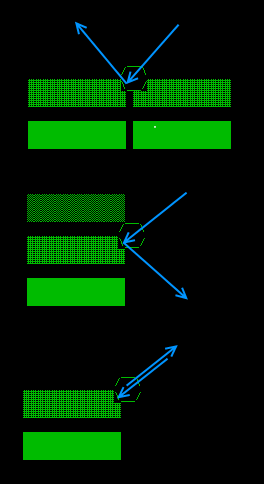
\includegraphics[scale=0.6]{figs/corner_reflex.png}
\caption{Boldens bevægelse når den rammer et hjørne}
\label{fig:cornerReflex}
\end{figure}

\underline{Flere brikker ramt.}\\

Som det kan ses på Figur \ref{fig:cornerReflex}, øverst, kan bolden ramme flere brikker af gangen. Når dette sker, skal man tjekke om der bare findes én brik på banen, hvor der er en konflikt med at reflektere bolden i en bestemt retning. Hvis der er det må brikken ikke reflekteres i denne retning.\\
Hvis man så på en situation hvor bolden kom oppefra og ramte øverste højre hjørne af en brik der havde en brik både til højre og ovenover den (en kombination af det øverste og midterste billede på Figur \ref{fig:cornerReflex} vil der både være en konflikt både i forhold til at reflektere bolden op og til siden. I denne specialsituation reflekteres bolden i begge retninger ligesom på det nederste billede i figuren.\\
\newpage

\underline{Briklogikken.}\\

Briklogikken er selve spillets game engine der styrer hvordan det opfører sig. Det er her alle reglerne for interaktion mellem bolden og brikkerne ligger. Når spillet itereres tjekker briklogikken om iterationen er gyldig. Et flowchart for briklogikken er vist på Figur \ref{fig:brickFlow}. De blå bokse på figuren repræsenterer funktionskald eller operationer på boldens vektors x- og y-koordinater. De grønne bokse er variable der bliver forøget eller sat (flagene dontDeflectX og dontDeflectY der bliver sat). De orange bokse er tests i form af if-statements. Med de grå bokse har vi vist alle indgange til, og udgange fra, det indlejrede for-loop der tjekker alle brikkerne
\footnote{Da et for-loop egentlig bare er noget kode der køres så længe en test er sand, kunne det tegnes med en orange boks og en pil der fører tilbage til den. For at forøge overskueligheden og holde antallet af test-bokse og lange pile i diagrammet nede, har vi dog valgt, at undlade at lave det på denne måde.}. De to gule bokse repræsenterer de samme linjer kode. Denne kode er en blanding af variable der bliver sat og funktioner der bliver kaldt hver gang logikken har gennemløbet en brik. \\

På Figur \ref{fig:brickFlow} kan det ses at der er adskillige steder hvor flagene \texttt{dontDeflectX} og \texttt{dontDeflectY} kan blive sat. Disse flag sættes hvis bolden ikke må blive reflekteret i en retning. De test der går forud for at et flag sættes, er altså reglerne for hvornår bolden ikke må reflekteres i en bestemt retning. 
Når bolden er itereret (øverste venstre hjørne på Figuren) kaldes briklogikken. Den funktion der itererer boldens position er \texttt{iterate()} der kan findes på linje 375 i \nameref{reflexball}.c der er vedlagt i Appendix \ref{C kode}. Denne funktion kalder \texttt{checkIteration(x,y)} på linje 145 i samme fil som er selve briklogikken. Briklogikken tester om iterationen er gyldig. Hvis den er det, tegnes bolden med \texttt{drawBigBall()}. Er den ikke det, reflekteres bolden hvorefter den tegnes. 

%\newpage

% Flowcharting techniques for easy maintenance
% Author: Brent Longborough
% =================================================
% Set up a few colours
%\colorlet{lcfree}{Green3}
%\colorlet{lcnorm}{Blue3}
%\colorlet{lccong}{Red3}
% -------------------------------------------------
% Set up a new layer for the debugging marks, and make sure it is on
% top
\pgfdeclarelayer{marx}
\pgfsetlayers{main,marx}
% A macro for marking coordinates (specific to the coordinate naming
% scheme used here). Swap the following 2 definitions to deactivate
% marks.
\providecommand{\cmark}[2][]{%
  \begin{pgfonlayer}{marx}
    \node [nmark] at (c#2#1) {#2};
  \end{pgfonlayer}{marx}
  } 
\providecommand{\cmark}[2][]{\relax} 
% -------------------------------------------------
% Start the picture
\begin{center}
\newgeometry{top=5cm, bottom=1cm, left=1cm, right=1cm}
\begin{figure}



\begin{tikzpicture}[%
    >=triangle 60,              % Nice arrows; your taste may be different
    start chain=going below,    % General flow is top-to-bottom
    node distance=4mm and 40mm, % Global setup of box spacing
    every join/.style={norm},   % Default linetype for connecting boxes
    scale=0.8, every node/.style={scale=0.9}
    ]
% ------------------------------------------------- 
% A few box styles 

% <on chain> *and* <on grid> reduce the need for manual relative
% positioning of nodes
\tikzset{
  base/.style={draw, on chain, on grid, align=center, minimum height=2ex},
  proc/.style={base, rectangle, fill=blue!30, font={\tiny}},
  test/.style={base, diamond, aspect=2.2, fill=orange!40, font={\tiny}},
  term/.style={proc, rounded corners,fill=green!30, font={\tiny}},
  placeholder/.style={base, on chain, text width=6em, fill=white, font={\tiny}},
  % coord node style is used for placing corners of connecting lines
  coord/.style={coordinate, on chain, on grid, node distance=4mm and 4mm},
  % nmark node style is used for coordinate debugging marks
  nmark/.style={draw, cyan, circle, font={\sffamily\bfseries}},
  % -------------------------------------------------
  % Connector line styles for different parts of the diagram
  norm/.style={->, draw},
  free/.style={->, draw},
  cong/.style={->, draw},
  it/.style={font={\tiny}}
}
% -------------------------------------------------
% Start by placing the nodes
\node [proc, it] (p0) {Iterate ball};
\node [test, join] (t0) {Indenfor bane?};

% No join for exits from test nodes - connections have more complex
% requirements
% We continue until all the blocks are positioned
\node [proc, fill=gray!30] (p1) {For(alle brikker)};
\node [test, join]	(t1)	{Ramt brik?};
\node [term]    	(p2) 	{score++};
\node [test, join]	(t2) 	{Top/bund?};
\node [test] 		(t3)	{DeflectedY?};
\node [test] 		(t4) 	{Top, ven- \\ stre/højre?};
\node [test] 		(t5)	{Brik over?};
\node [term]  		(p3)    {dontDeflectY};

\node [placeholder, opacity=0] {};
\node [placeholder, opacity=0] {};
\node [placeholder, opacity=0] {};
\node [placeholder, opacity=0] {};
\node [placeholder, opacity=0] {};

\node [test]		(t8)  {Ramt midt \\ i brikken?};
\node [term]  		(p5)  {dontDeflectY};
\node [test, join]	(t9)  {Top fra neden?};
\node [term]		(p6)	  {dontDeflectY};


\node [test, join]	(t11)		{dontDeflectY?};
\node [proc, it] 	(p8) 		{Reflekter Y};


% We position the next block explicitly as the first block in the
% second column.  The chain 'comes along with us'. The distance
% between columns has already been defined, so we don't need to
% specify it.
%%%% NÆSTE KOLONNE
\node [placeholder, opacity=0, right=of t0] (k0) {};

\node [proc, it, fill=gray!30, right=of t1]  (e1) {Næste brik i \\ for-loop};

\node [placeholder, opacity=0, right=of t4]  {};
\node [test] 	(t6) {Bund, ven- \\ stre/højre?};
\node [test]				(t7) {Brik under?};
\node [term]      	  		(p4) {dontDeflectY};

\node [test, right=of t9] 	(t10)  	{Bund fra oven?};
\node [term]      			(p7)	{dontDeflectY};


%%%% NÆSTE KOLONNE
\node [placeholder, opacity=0, right=of k0]  {};
\node [test] 	(t12) {Side? \& !xDeflected};
\node [test] 				(t13) {Top/bund?};
\node [test] 				(t14) {Venstre \& \\ brik til venstre?};
%\node [test] (t14) {Levende brik til venstre?};
\node [term] 				(p9)  {dontDeflectX};
\node [test, join] 			(t15) {Højre side \& \\ brik til højre?};
%\node [test] (t16) {Levende brik til højre?};
\node [term]      			(p10)  {dontDeflectX};

\node [placeholder, opacity=0]  (k3) {};
\node [test, join] 	(t16) {Venstre side?};
\node [test] 		(t17) {Kommer fra \\ højre?};
\node [term]      	(p11) {dontDeflectX};
% Tre til højre for som er under i hieraki

\node [placeholder, opacity=0]  {};
\node [test] 	(t20) {Fra siden, \\ ml. top \\ og bund?};
\node [test] 		(t21) {Top?};
\node [test] 		(t22) {Fra oven \& \\ frit over?};
\node [term]      	(p13) {dontDeflectX};
\node [test, join] 	(t24) {dontDeflectX?};
\node [proc, it] 	(p15) {Reflekter X};


%%\node [test] (t19) {Højre side?};
%%%%% NÆSTE KOLONNE
%\node [placeholder, opacity=0, right=of t12] (k1) {};
\node [proc, it, right=of t12] 			(k1) {Spilleren er død};
\node [proc, it, fill=yellow!30, right=of t13] (e0) {Herefter følger koden \\  i den gule boks nedenfor};
\node [test, right=of t16] 	(t18) {Højre side?};
\node [test] 				(t19) {Kommer fra \\ venstre?};
\node [term]      			(p12) {dontDeflectX};

\node [test, right=of t22] 	(t23) {Fra neden \& \\ frit under?};
\node [term]    			(p14) {dontDeflectX};
\node [proc, it, fill=yellow!30, right=of p15]  (e2) {brick.lives- - \\ Tegn brik \\ Drej random vinkel };

%%%%% NÆSTE KOLONNE
\node [test, right=of k1] 	(t25) {Under striker?};
\node [test] 				(t26) {gameStarted?};
\node [test] 				(t27) {Udenfor sider?};
\node [proc, it] 			(p16) {Reflekter X};
\node [test, join]			(t28) {Over top/ \\ på striker?};
\node [test] 				(t29) {Ramt striker?};
\node [proc] 				(p17) {Roter afhængigt \\ af hvor man rammer};
\node [proc, join] 			(p18) {Reflekter Y};

\node [proc, join] 			(p19) {drawBigBall \\ return};


\node [placeholder, opacity=0] {};
\node [placeholder, opacity=0] {};
\node [placeholder, opacity=0] {};

\node [proc, fill=gray!30] 			(e4) {Sidste brik i for-loop \\ går her til};
\node [test] 				(t30) {dontDeflectX \& \\ dontDeflectY?};
\node [proc] 			(e7) {Reflekter X \\ Reflekter Y};


\node [proc, it, fill=gray!30, right=of e2]  (e3) {Næste brik i \\ for-loop};








% -------------------------------------------------
% Now we place the coordinate nodes for the connectors with angles, or
% with annotations. We also mark them for debugging.
%\node [coord, right=of t1] (c1)  {}; %\cmark{1}   
%\node [coord, right=of t3] (c3)  {}; %\cmark{3}   
%\node [coord, right=of t6] (c6)  {}; %\cmark{6}   
%\node [coord, right=of t7] (c7)  {}; %\cmark{7}   
%\node [coord, left=of t4]  (c4)  {}; %\cmark{4}   
%\node [coord, right=of t4] (c4r) {}; %\cmark[r]{4}
%\node [coord, left=of t7]  (c5)  {}; %\cmark{5} 

% -------------------------------------------------

% -------------------------------------------------
% All the other connections come out of tests and need annotating
% First, the straight north-south connections. In each case, we first
% draw a path with a (consistently positioned) annotation node, then
% we draw the arrow itself.
\path (t0.south) to node [near start, xshift=1em] {$ja$} (p1);
  \draw [->] (t0.south) -- (p1);
 
\path (t1.south) to node [near start, xshift=1em] {$ja$} (p2);
  \draw [->] (t1.south) -- (p2);
  
\path (t2.south) to node [near start, xshift=1em] {$ja$} (t3);
  \draw [->] (t2.south) -- (t3);  

\path (t3.south) to node [near start, xshift=1em] {$nej$} (t4);
  \draw [->] (t3.south) -- (t4);
  
\path (t4.south) to node [near start, xshift=1em] {$ja$} (t5);
  \draw [->] (t4.south) -- (t5);

\path (t5.south) to node [near start, xshift=1em] {$ja$} (p3);
  \draw [->] (t5.south) -- (p3); 

\path (t8.south) to node [near start, xshift=1em] {$ja$} (p5);
  \draw [->] (t8.south) -- (p5);
  
\path (t9.south) to node [near start, xshift=1em] {$ja$} (p6);
  \draw [->] (t9.south) -- (p6); 
  
\path (t11.south) to node [near start, xshift=1em] {$nej$} (p8);
  \draw [->] (t11.south) -- (p8);
  
%%Næste række (mellemrække)
\path (t6.south) to node [near start, xshift=1em] {$ja$} (t7);
  \draw [->] (t6.south) -- (t7);
 
\path (t7.south) to node [near start, xshift=1em] {$ja$} (p4);
  \draw [->] (t7.south) -- (p4);
  
\path (t10.south) to node [near start, xshift=1em] {$ja$} (p7);
  \draw [->] (t10.south) -- (p7);

%%Næste række
\path (t12.south) to node [near start, xshift=1em] {$ja$} (t13);
  \draw [->] (t12.south) -- (t13); 
  
\path (t13.south) to node [near start, xshift=1em] {$ja$} (t14);
  \draw [->] (t13.south) -- (t14);

\path (t14.south) to node [near start, xshift=1em] {$ja$} (p9);
  \draw [->] (t14.south) -- (p9); 

\path (t15.south) to node [near start, xshift=1em] {$ja$} (p10);
  \draw [->] (t15.south) -- (p10); 

\path (t16.south) to node [near start, xshift=1em] {$ja$} (t17);
  \draw [->] (t16.south) -- (t17); 

\path (t17.south) to node [near start, xshift=1em] {$ja$} (p11);
  \draw [->] (t17.south) -- (p11);

\path (t20.south) to node [near start, xshift=1em] {$ja$} (t21);
  \draw [->] (t20.south) -- (t21);
  
\path (t21.south) to node [near start, xshift=1em] {$ja$} (t22);
  \draw [->] (t21.south) -- (t22);  

\path (t22.south) to node [near start, xshift=1em] {$ja$} (p13);
  \draw [->] (t22.south) -- (p13);

\path (t24.south) to node [near start, xshift=1em] {$nej$} (p15);
  \draw [->] (t24.south) -- (p15);
  

% Næste række (mellemrække)
\path (t18.south) to node [near start, xshift=1em] {$ja$} (t19);
  \draw [->] (t18.south) -- (t19);

\path (t19.south) to node [near start, xshift=1em] {$ja$} (p12);
  \draw [->] (t19.south) -- (p12);

\path (t23.south) to node [near start, xshift=1em] {$ja$} (p14);
  \draw [->] (t23.south) -- (p14);


% Næste række
\path (t25.south) to node [near start, xshift=1em] {$nej$} (t26);
  \draw [->] (t25.south) -- (t26);

\path (t26.south) to node [near start, xshift=1em] {$ja$} (t27);
  \draw [->] (t26.south) -- (t27);
  
\path (t27.south) to node [near start, xshift=1em] {$ja$} (p16);
  \draw [->] (t27.south) -- (p16);
  
\path (t28.south) to node [near start, xshift=1em] {$ja$} (t29);
  \draw [->] (t28.south) -- (t29);
  
\path (t29.south) to node [near start, xshift=1em] {$ja$} (p17);
  \draw [->] (t29.south) -- (p17);




%\path (t6.south) to node [near start, xshift=1em] {$y$} (t7); 
% \draw [*->,lcfree] (t6.south) -- (t7); 
% ------------------------------------------------- 
% Now the straight east-west connections. To provide consistent
% positioning of the test exit annotations, we have positioned
% coordinates for the vertical part of the connectors. The annotation
% text is positioned on a path to the coordinate, and then the whole
% connector is drawn to its destination box.
%\path (t3.east) to node [near start, yshift=1em] {$n$} (c3); 
%  \draw [o->,lccong] (t3.east) -- (p8);
%\path (t4.east) to node [yshift=-1em] {$k \leq 0$} (c4r); 
%  \draw [o->,lcnorm] (t4.east) -- (p9);

% -------------------------------------------------
% The coordinates

\node [coord, right = 20mm of p1] (cp1)  {}; %\cmark{1}
\node [coord, right = 20mm of t1] (ct1)  {}; %\cmark{1}
\node [coord, right = 20mm of t4] (ct4)  {}; %\cmark{1} 
\node [coord, below = of p3] (cp3)  {}; %\cmark{1}
\node [coord, right = 20mm of t5] (ct5)  {}; %\cmark{1}

\node [coord, right = 18mm of t8] (ct8)  {}; %\cmark{1}
\node [coord, below = of p5] (cp5)  {}; %\cmark{1}
\node [coord, right = 22mm of p5] (cp5r)  {}; %\cmark{1}
\node [coord, right = 22mm of t9] (ct9)  {}; %\cmark{1}

\node [coord, right = 22mm of t11] (ct11)  {}; %\cmark{1}
\node [coord, below = 20 mm of ct11] (cp8)  {}; %\cmark{1}
\node [coord, right = 40 mm of cp8] (cp8r)  {}; %\cmark{1}



% Næste kolonne (mellemrække)
\node [coord, below = of p4] (cp4)  {}; %\cmark{1}
\node [coord, right = 20mm of t6] (ct6)  {}; %\cmark{1}
\node [coord, right = 20mm of t7] (ct7)  {}; %\cmark{1}
\node [coord, right = 18mm of t10] (ct10)  {}; %\cmark{1}
\node [coord, below = of p7] (cp7)  {}; %\cmark{1}


% Næste kolonne

\node [coord, below = of t0] (ct0b)  {}; %\cmark{1}
\node [coord, right = 62 mm of ct0b] (ct12)  {}; %\cmark{1}
\node [coord, right = 62 mm of t2] (ct2r)  {}; %\cmark{1}
\node [coord, right = 62 mm of t3] (ct3r)  {}; %\cmark{1}


\node [coord, right = 23 mm of t13] (ct13)  {}; %\cmark{1}


\node [coord, right = 20 mm of t14] (ct14)  {}; %\cmark{1}
\node [coord, below = of p9] (cp9)  {}; %\cmark{1}

\node [coord, right = 20 mm of t15] (ct15)  {}; %\cmark{1}
\node [coord, below = of p10] (cp10)  {}; %\cmark{1}
\node [coord, right = 20 mm of cp10] (cp10r)  {}; %\cmark{1}

\node [coord, below = of p11] (cp11)  {}; %\cmark{1}
\node [coord, below = of cp11] (cp11b)  {}; %\cmark{1}

\node [coord, below = of k3] (ck3b)  {}; %\cmark{1}
\node [coord, right = 22 mm of ck3b] (ck3)  {}; %\cmark{1}
\node [coord, right = 22 mm of t16] (ct16)  {}; %\cmark{1}
\node [coord, right = 22 mm of t17] (ct17)  {}; %\cmark{1}

\node [coord, right = 20 mm of t18] (ct18)  {}; %\cmark{1}
\node [coord, right = 20 mm of t19] (ct19)  {}; %\cmark{1}

\node [coord, below = of p13] (cp13)  {}; %\cmark{1}
\node [coord, right = 21 mm of cp13] (cp13r)  {}; %\cmark{1}

\node [coord, below = of p14] (cp14)  {}; %\cmark{1}
\node [coord, right = 21 mm of t23] (ct23)  {}; %\cmark{1}
\node [coord, right = 22 mm of t20] (ct20)  {}; %\cmark{1}

%Sidste kolonne
\node [coord, right = 22 mm of t0] (ct0r)  {}; %\cmark{1}
\node [coord, left = 18 mm of t27] (ct27)  {}; %\cmark{1}
\node [coord, left = 16 mm of t29] (ct29)  {}; %\cmark{1}

\node [coord, below = of p16] (cp16)  {}; %\cmark{1}
\node [coord, below = 6mm of p17] (cp17)  {}; %\cmark{1}
\node [coord, below = of p18] (cp18)  {}; %\cmark{1}
\node [coord, left = 18 mm of cp16] (cp16l)  {}; %\cmark{1}
\node [coord, left = 16 mm of cp17] (cp17l)  {}; %\cmark{1}
\node [coord, right = 18 mm of cp18] (cp18r)  {}; %\cmark{1}

\node [coord, right = 18 mm of t26] (ct26)  {}; %\cmark{1}
\node [coord, right = 18 mm of t28] (ct28)  {}; %\cmark{1}

\node [coord, below = of t12] (ct12b)  {}; %\cmark{1}
\node [coord, right = 18 mm of ct12b] (ct12br)  {}; %\cmark{1}

\node [coord, right = 18 mm of t30] (ct30r)  {}; %\cmark{1}
\node [coord, below = 10mm of e7] (ct30b)  {}; %\cmark{1}
\node [coord, right = 18 mm of ct30b] (ct30br)  {}; %\cmark{1}

% -------------------------------------------------
% Finally, the twisty connectors. Again, we place the annotation
% first, then draw the connector

\path (t0.east) to node [very near start, yshift=1em] {$nej$} (ct0r); 
  \draw [->] (t0.east) -- (ct0r) -| (t25);
  
\path (t25.west) to node [very near start, yshift=1em] {$ja$} (k1); 
  \draw [->] (t25.west)  --(k1);

\path (t27.west) to node [very near start, yshift=1em] {$nej$} (ct27); 
  \draw [->] (t27.west)  --(ct27) |- (cp16l) -|(t28);
  
\path (t29.west) to node [very near start, yshift=1em] {$nej$} (ct29); 
  \draw [->] (t29.west)  --(ct29) |- (cp17l) -|(p18);

\path (t26.east) to node [very near start, yshift=1em] {$nej$} (ct26); 
  \draw [->] (t26.east)  --(ct26) |- (cp18r) -|(p19);
  
\path (t28.east) to node [very near start, yshift=1em] {$nej$} (ct28); 
  \draw [->] (t28.east)  --(ct28);
  
\path (e4.south) to node [very near start, yshift=1em] {} (t30); 
  \draw [->] (e4.south)  --(t30);
  

\path (t30.south) to node [very near start, xshift=1em, yshift=0.5em] {$ja$} (ct30b); 
  \draw [->] (t30.south) -- (e7);

\path (e7.south) to node [very near start, yshift=1em] {} (ct30b); 
  \draw [->] (e7.south)  |- (ct30b) -| (ct30br) -| (cp18r);
  
\path (t30.east) to node [very near start, yshift=1em, xshift=-0.5em] {$nej$} (ct30r); 
  \draw [->] (t30.east)  -- (ct30r); 
  
  
\path (t12.east) to node [very near start, yshift=1em] {$nej$} (ct12br); 
  \draw [->] (t12.east)  -| (ct12br) -| (e0);
%% Slut..! nedenfor er starten


\path (t1.east) to node [very near start, yshift=1em] {$nej$} (e1); 
  \draw [->] (t1.east) -- (e1) ;
  
%\path (e1.north) to node [very near start, yshift=1em] {} (p1); 
%  \draw [->] (e1.north) -- (p1) ;

\path (t2.east) to node [very near start, yshift=1em] {$nej$} (ct2r); 
  \draw [->] (t2.east) -- (ct2r);

\path (t3.east) to node [very near start, yshift=1em] {$nej$} (ct3r); 
  \draw [->] (t3.east) -- (ct3r); 
  
\path (t4.east) to node [very near start, yshift=1em] {$nej$} (t6); 
  \draw [->] (t4.east) -| (t6);

\path (p3.south) to node [very near start, yshift=1em] {} (cp3); 
  \draw [->] (p3.south) |- (cp3) -| (ct4);

\path (t5.east) to node [very near start, yshift=1em] {$nej$} (ct5); 
  \draw [->] (t5.east) -- (ct5);

\path (t8.east) to node [very near start, yshift=1em] {$nej$} (ct8); 
  \draw [->] (t8.east) -| (ct8) |- (cp5) -| (t9);

\path (t9.east) to node [very near start, yshift=1em] {$nej$} (ct9); 
  \draw [->] (t9.east) -| (ct9) |- (cp5r) -| (t10) ;

\path (t11.east) to node [very near start, yshift=1em] {$nej$} (ct11); 
  \draw [->] (t11.east) -- (ct11) -| (cp8); 
  
\path (p8.south) to node [very near start, yshift=1em] {} (cp8); 
  \draw [->] (p8.south) |- (cp8) -- (cp8r) |- (ct12) -| (t12); 


  
  
  
% Næste kolonne (mellemkolonne)  
\path (p4.south) to node [very near start, yshift=1em] {} (cp4); 
  \draw [->] (p4.south) -| (cp4) -| (t8);
  
\path (t6.east) to node [very near start, yshift=1em] {$nej$} (ct6); 
  \draw [->] (t6.east) -| (ct6) |- (cp4);

\path (t7.east) to node [very near start, yshift=1em] {$nej$} (ct7); 
  \draw [->] (t7.east) -- (ct7);
  
\path (t7.east) to node [very near start, yshift=1em] {$nej$} (ct7); 
  \draw [->] (t7.east) -- (ct7);

\path (p7.south) to node [very near start, yshift=1em] {} (cp7); 
  \draw [->] (p7.south) |- (cp7) -| (t11);

\path (t10.east) to node [very near start, yshift=1em] {$nej$} (ct10); 
  \draw [->] (t10.east) -| (ct10) |- (cp7);
  


% Næste kolonne 

\path (t14.east) to node [very near start, yshift=1em] {$nej$} (ct14); 
  \draw [->] (t14.east) -- (ct14) |-(cp9) -| (t15);
  
\path (t15.east) to node [very near start, yshift=1em] {$nej$} (ct15); 
  \draw [->] (t15.east) -- (ct15) |-(cp10) -| (t16);
  
\path (t13.east) to node [very near start, yshift=1em] {$nej$} (ct13); 
  \draw [->] (t13.east) -- (ct13) |-(cp10r) ;

\path (p11.south) to node [very near start, yshift=1em] {} (cp11); 
  \draw [->] (p11.south) |- (cp11) -|(ck3) -| (t18) ;
  
\path (t16.east) to node [very near start, yshift=1em] {$nej$} (ct16); 
  \draw [->] (t16.east) -- (ct16);

\path (t17.east) to node [very near start, yshift=1em] {$nej$} (ct17); 
  \draw [->] (t17.east) -- (ct17);


\path (p12.south) to node [near start, yshift=1em] {} (cp11b); 
  \draw [->] (p12.south) |- (cp11b) -| (t20);
  
\path (t18.east) to node [very near start, yshift=1em] {$nej$} (ct18); 
  \draw [->] (t18.east) -| (ct18) |- (cp11b) -|(t20) ; 

\path (t19.east) to node [very near start, yshift=1em] {$nej$} (ct19); 
  \draw [->] (t19.east) -- (ct19) ; 

\path (t21.east) to node [very near start, yshift=1em] {$nej$} (t23); 
  \draw [->] (t21.east) -| (t23) ; 
  
\path (t22.east) to node [very near start, yshift=1em] {$nej$} (cp13r); 
  \draw [->] (t22.east) -| (cp13r) ; 
  
\path (p14.south) to node [near start, yshift=1em] {} (cp14); 
  \draw [->] (p14.south) |- (cp14) -| (t24);

\path (t20.east) to node [near start, yshift=1em] {$nej$} (ct20); 
  \draw [->] (t20.east) -- (ct20) -| (ct23); 

\path (t23.east) to node [very near start, yshift=1em] {$nej$} (ct23); 
  \draw [->] (t23.east) -- (ct23) |- (cp14) ; 
  
\path (p15.east) to node [very near start, yshift=1em] {} (e2); 
  \draw [->] (p15.east) -- (e2);

\path (e2.east) to node [very near start, yshift=1em] {} (e3); 
  \draw [->] (e2.east) -- (e3);      


%\path (t1.east) to node [near start, yshift=1em] {$n$} (c1); 
%  \draw [o->,lcfree] (t1.east) -- (c1) |- (p4);
%\path (t2.east) -| node [very near start, yshift=1em] {$n$} (c1); 
%  \draw [o->,lcfree] (t2.east) -| (c1);
%\path (t4.west) to node [yshift=-1em] {$k>0$} (c4); 
%  \draw [*->,lcnorm] (t4.west) -- (c4) |- (p3);
%\path (t5.east) -| node [very near start, yshift=1em] {$n$} (c6); 
%  \draw [o->,lcfree] (t5.east) -| (c6); 
%\path (t6.east) to node [near start, yshift=1em] {$n$} (c6); 
%  \draw [o->,lcfree] (t6.east) -| (c7); 
%\path (t7.east) to node [yshift=-1em] {$k \leq 0$} (c7); 
%  \draw [o->,lcfree] (t7.east) -- (c7)  |- (p9);
%\path (t7.west) to node [yshift=-1em] {$k>0$} (c5); 
%  \draw [*->,lcfree] (t7.west) -- (c5) |- (p5);
% -------------------------------------------------
% A last flourish which breaks all the rules
%\draw [->,MediumPurple4, dotted, thick, shorten >=1mm]
%  (p9.south) -- ++(5mm,-3mm)  -- ++(27mm,0) 
%  |- node [black, near end, yshift=0.75em, it]
%   {(When message + resources available)} (p0);
% -------------------------------------------------



\end{tikzpicture}
\caption{Flowchart for briklogikken der styrer interaktionen mellem brikkerne og bolden}
\label{fig:brickFlow}
\end{figure}
\restoregeometry
\end{center}


		

\section{Helhedsindtryk}


\underline{LED display med score, liv og levels}\\

Udover at vise brugerens score, liv og nuværende level på skærmen, valgte vi også at bruge boardet indbyggede LED display til at vise dette. På den måde kan brugeren se hans score når spillet kører og hans liv hver gang han dør eller går et level up. \\
For at vise de forskellige karakterer på displayet opsatte vi Timer2 til at inerrupte hver 500us, den kalder derefter en funktion der sørger for at  multiplekse LED displayet, så hurtigt at det virker som om alle LED'er hele tiden er tændt. Oprindeligt kaldte vi opdaterings funktionen fra vores main-loop, men det bevirkede i at displayet blinkede, da der var forholdsvis lange pauser hver gang den skulle opdaterer spillet. \\

Da funktionen bliver kaldt inde i et interrupt er det nødvendigt at sikre sig at denne er så kort som mulig, så programmet ikke bruger for lang tid på at eksekvere interruptet. Dette sikrede vi ved kun at gemme de første 5 karakterer i en video-buffer og derefter læse fra den ved at læse direkte fra en specifik adresse i microcontrollerens memory. Derved undgår man at skulle flytte rundt på video-bufferen hele tiden, der ville tage meget lang tid at eksekverer. Man skal dog selv holde styr på at man ikke læser fra et andet sted i hukommelsen. \\

Koden til opdaterings-funktionen kan ses nedenfor.

\begin{lstlisting}[frame=single]
PGOUT = (PGOUT & (1 << 7)) | *(&videoBuffer[0][0] + digit*6 + column + index);
PEOUT |= 0x1F; // Set all cathodes high
PEOUT &= ~(1 << (4-column)); // Set one cathodes low decided by column

clockLed(digit);
if (++digit == 4) {
  digit = 0;
  if (++column == 5) {
    column = 0;
	if (++delayCounter == SCROLL_SPEED && stringLength > 4) { // We don't have to scroll the text if there is less than five characters
	  delayCounter = 0;				
	  if (++index > 5) {
        index = 0;
		moveVideoBuffer();
	  }
	}
  }
}
\end{lstlisting}

Det ses i linje 1, at vi blot lægger et tal til video-bufferens adresse, dette tager således utroligt lidt tid og dermed opstår der ingen problemer ved at kalde den i et interrupt. Som det ses i linje 14 skal den dog stadig flytte bufferen hver gang den kommer til en ny karakter. Denne kode kan ses i afsnittet \nameref{LED} i appendiks.\\

Udover at kunne scolle den samme tekst havde vi også brug for at kunne scrolle en besked én gang på displayet - dette bruger vi fx hver gang man dør eller går til næste level.\\

Funktionen \texttt{LEDRunOnce()} kan ses nedenfor.
\newpage

\begin{lstlisting}[frame=single]
// Used to sroll the first string once and then show the second string afterwards
void LEDRunOnce(char *firstString, char* secondString) {
	LEDsetString(firstString);
	runOnce = 1;
	pSecondString = secondString; // We will save the location of the second string
}
\end{lstlisting}

Den virker på den måde at den sætter den første streng på normalvis, den sætter dog flaget \texttt{runOnce()} til 1 og derefter sætter den en pointer til den anden streng.\\

Et udsnit af funktionen \texttt{moveVideoBuffer()} kan ses nedenfor.

\begin{lstlisting}[frame=single,firstnumber=12]
pString++;
if (*pString == '\0') { // Check if we have reached the end of the string
  if (runOnce) { // This wil actually abort when it loads the last character in the 5th digit, so you have to put a space in end of the sentence
    runOnce = 0;
	LEDsetString(pSecondString);
  } else
	pString -= stringLength;
}
\end{lstlisting}

Når den kommer til null-terminatoren i strengen tjekker den om det var funktionen \texttt{LEDRunOnce()} der blev kaldt. Hvis dette var tilfældet kalder den \texttt{LEDsetString()} med pointen til den anden streng som argument.\\

\underline{Menu hvor man kan vælge sværhedsgrad}\\

For at kunne variere spillets sværhedsgrad implementerede vi et menu system i starten af spillet hvor brugeren kan vælge den ønskede sværhedsgrad. Et screenshot af menuen kan ses i se figur \ref{fig:menu}. Menuen står og kører i et while-loop indtil brugeren har valgt en sværhedsgrad.

\begin{figure}[h!]
\centering
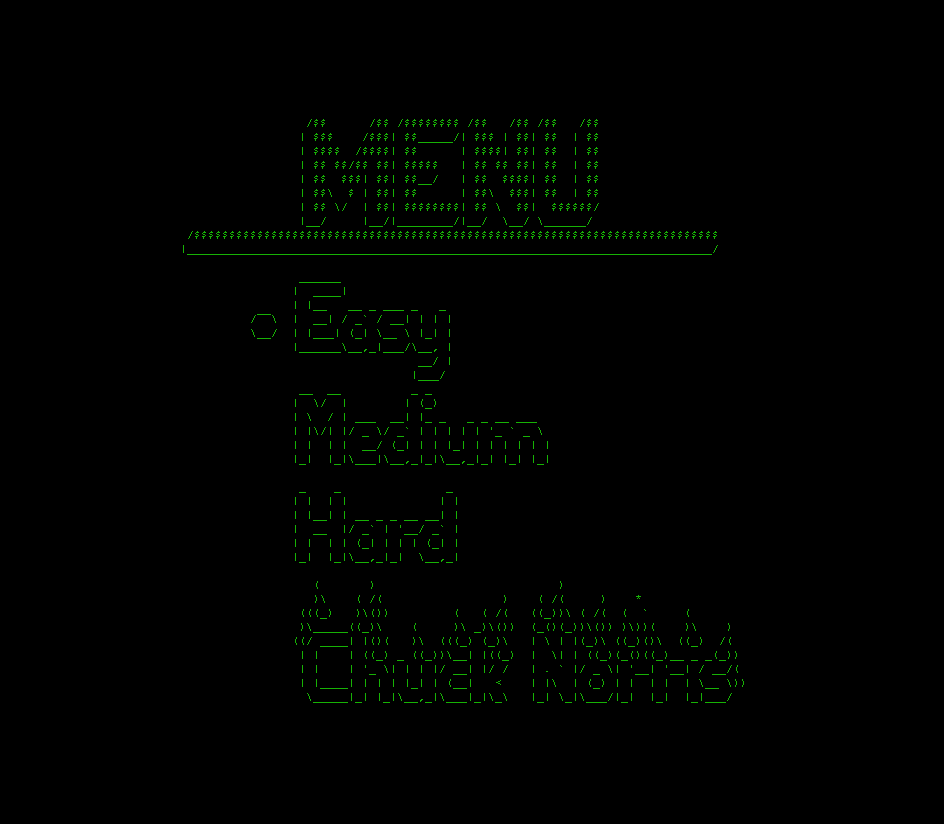
\includegraphics[scale=0.25]{figs/screenshots/menu_crop.png}
\caption{Screenshot af menuen}
\label{fig:menu}
\end{figure}

\underline{Beskeder ved Game Over}\\

Når spilleren dør vises en fast tekst "GameOver", samt et vilkårligt citat. I alt er der 8 forskellige citater som kan vises når man dør. En eksempel på dette kan ses i figur \ref{fig:gameover}.

\begin{figure}[h!]
\centering

\includegraphics[scale=0.25]{figs/screenshots/gameover_crop.png}
\caption{Eksempel på screenshot game over tekst}
\label{fig:gameover}
\end{figure}

For at kunne vælge en tilfældig tekst benytter vi os af at funktionen \texttt{millis()} nederste bits ændrer sig meget hurtigt. Ved at læse de tre nederste bits kan vi således få et "tilfældigt" tal mellem 0-7. Den er dog ikke helt tilfældig, men i stedet det man kalder pseudo-tilfældig - dette er dog tilstrækkeligt i dette tilfælde.\\

Det udsnit af funktionen \texttt{showGameOver()} der læser \texttt{millis()} kan ses nedenfor.

\begin{lstlisting}[frame=single,firstnumber=6]
switch (millis() & 0x7) { // Pseudo random number from 0-7
\end{lstlisting}

\underline{Besked hvis spillet vindes}\\

Hvis man er så heldig at vinde spillet vises der en lykønskning samt en opkvikker i form af en flot præmiepige, da dette er ægte klassisk japansk arkade coutume.\\

Figur \ref{fig:won_normal} viser et screenshot ved gennemførsel af spillet.\\

\begin{figure}[h!]
\centering

\includegraphics[scale=0.25]{figs/screenshots/won_normal.png}
\caption{Screenshot ved gennemførsel af spillet}
\label{fig:won_normal}
\end{figure}

\underline{Implementering af ASCII-Art}\\

For let at kunne genere et array der kan sættes direkte ind i C-koden, lavede vi et Java-program der kan åbne et billede i ASCII-art og indsætte de nødvendige escape backslashes i filen samt bestemme længden og højden af array'et. Koden til programmet kan ses i afsnittet \nameref{BackslashEscapes} i appendiks.
\newpage

\section{Styring med rat}
Som et delmål fandt vi hurtigt ud af vi ville have et DEXXA Steering Wheel sluttet til microcontrolleren, sådan så styringen af strikeren var væsentlig bedre i forhold til keyboardet eller udviklings boardets indbyggede knapper.\\

\underline{Gameport adapter}\\

For at kunne koble DEXXA Steering Wheel'et til vores udviklingsboard var det dog nødvendigt at lave en lille adapter. På den måde kan vi aflæse alle digitale knapper samt de to potentiometre inde i rattet og pedalerne - vi bruger dog ikke pedalerne i spillet.\\

De digitale knapper fungerer ved at de er forbundet til en række knapper der svæver når de ikke holdes i bund. Hvis knappen holde nede kortsluttes den til \texttt{GND}. Ved at forbinde indgangen til knappen til en pullup modstand og derefter forbinde indgangen til en indgang på microcontrolleren kan man således aflæse knapperne. Udover at forbinde en pullup modstand til indgangen forbandt vi også en 100nF kondensator for at modvirke debouncing.\\

Rattet og pedalerne fungerer en smule anderledes i det de er forbundet til et 100k$\Omega$ potentiometer. Potentiometerets ene ben er forbundet til \texttt{VCC}, mens det andet er forbundet til en udgang på Gameporten. Ved at forbinde denne udgang til en 100k$\Omega$ modstand der er forbundet til \texttt{GND} har man således dannet en spændingsdeler vha. de to modstande. Ved at måle spændingen vha. ADC'en i microcontrolleren kan man således bestemme positionen af rattet og pedalerne.\\

Koden til at læse en analog indgang kan ses nedenfor.

\begin{lstlisting}[frame=single]
unsigned int readADC(unsigned char channel) { // Read a specific analog channel
  unsigned char inHigh, inLow;
  unsigned int ADC_data;
  
  ADCCTL = 0x80 | 0x20 | (channel & 0x0F); // Enable ADC on the selected channel and use external voltage (3.3V) as VREF
  while (ADCCTL & 0x80); // Wait for conversion to be completed
  inHigh = ADCD_H; // ADC high byte
  inLow = ADCD_L; // ADC low low byte
  ADC_data = ((unsigned int)inHigh << 2)| inLow >> 6; // ADC output word
  
  return ADC_data;
}
\end{lstlisting}

På linje 5 opsættes ADC'en til at starte målingen på den pågældende indput. Derudover benytter vi os af en ekstern spændings reference på 3.3V. I linje 6 venter koden på at ADC konverteringen er færdig, når dette sker cleares bit 7 og koden aflæser nu de to registre og returnerer spændingen som en 10-bit værdi mellem 0-1023.\\
Først lavede vi lineær model for rattet, men det viste sig hurtigt at den ikke var lineær, derfor lavede vi blot inddelingen manuelt vha. en række if-sætning.\\

Den samlede koden til Gameport adapteren kan ses i \nameref{gameport} i appendiks.\\

Et pinout til Gameport'en samt dybere forklaring kan ses på følgende side \footnote{\url{http://pinouts.ru/Inputs/GameportPC_pinout.shtml}} .\\

Figur \ref{fig:board_overview} nedenfor viser hvordan Gameport adapteren er forbundet til udviklingsboardet.

\begin{figure}[h!]
\centering
\includegraphics[scale=0.10]{figs/board_overview_crop.png}
\caption{Billede af Gameport adapteren forbundet til udviklings boardet}
\label{fig:board_overview}
\end{figure}
\newpage

\underline{Styring med intern hardware og keyboard}\\

Udover at kunne styre spillet vha. rattet kan man også styre spillet vha. computerens keyboard eller udviklings boardets knapper. Spillet er dog tiltænkt at skulle styres med rattet, da det giver en meget bedre styringsfølsomhed og dermed en bedre spilleoplevelse.\\

\section{Rettelser og fintuning}


\underline{Bolden bevæger sig med samme hastighed i både x- og y-retning}\\

Vi havde et problem med at det på skærmen lignede at boldens hastighed variede meget afhængigt af om dens vektor var relativt vandret (lille absolut y-komposant) eller relativt lodret (lille x-komposant). Dette skyldes at monospace-karakteren er meget tæt på at være dobbelt så høj som den er bred. Vores løsningen på dette var at gøre boldens vektors x-komposant dobbelt så stor, ved at bitshifte den 1 til venstre. På den måde er bolden ikke længere en enhedsvektor med mindre dens x-komposant er nul.\\
Når bolden så rammer ind i noget bitshiftes \texttt{ball.vector.x} 1 til højre (divideres med to), for at gøre boldens vektor til enhedsvektor igen, sådan så der ikke opstår rod når boldens vektor roteres.\\

\underline{Skift til Putty Terminal}\\

Som en del af de avancerede mål, skiftede vi fra Hyper Terminal over til Putty Terminal. Den eneste grund til dette er man i Putty Terminal kan lave meget større opløsning, sådan så spillet ser flottere ud og kan spilles som et fullscreen-spil. De eneste komplikationer der var forbundet med dette var at nogle få af ASCII-karaktererne blev tegnet på en anden måde i Putty end tiltænkt, selvom både Hyper og Putty terminalerne bruger charset 850. Løsningen på dette var bare at bruge nogle andre ASCII-karakterer.\\

\underline{Implementering af en lille smule vilkårlighed ved hver afbøjning}\\

Som i professionelle computerspil, har vi sørget for at implementere en mindre vilkårlighed i hvor meget bolden afbøjes hver gang den roteres, dvs. både når den rammer striker, brikker, loft eller vægge. Bolden får da sin almindelige beregnede afbøjningsvinkel med en adderet pseudovilkårlig rotation på mellem minus 3 og plus 4 ud af 512. Det vil sige en vinkel på mellem ca. minus 2,1 og plus 2,8 grader. Dette er en vinkel lille nok til man med øjet aldrig ved ligge mærke til afbøjningsvinklen ikke er er helt lig med indgangsvinklen på brikker, loft og vægge, men samtidig stor nok til at bolden ikke bliver reflekteret rundt sådan at den er fanget i et fast mønster.\\

\underline{Justering af hvor ofte bolden tegnes}\\

Som nævnt i afsnit \textbf{3.2} havde vi lidt problemer med at uarten ikke altid kunne tegne bolden hurtigt nok, efter vi lavede bolden til at fylde 4x2 monospace-karakterer. Vi oplevede at hvis delayet mellem aftegningerne af bolden blev for lille, så kunne man risikere ofte ikke at kunne se bolden, da vores kode jo er lavet på den måde at bolden først slettes, derefter bevæger sig og så tegnes igen. Altså uarten kunne ikke nå at gennemføre hele processen med det resultat at boldene kun slettedes og ikke blev tegnet ordentligt op igen. Desuden opleve vi flere gange at terminalen frøs, hvis vi prøvede at tegne bolden for hurtigt.\\
Som en løsning på dette justerede vi hastigheden sådan så når der er under 20ms delayet mellem aftegningerne af bolden, så tegnes den kun hver anden gang. Dette letter arbejdet for uarten nok til at det bolden ser ordentlig ud hele tiden. Vi eksperimenterede også med kun at tegne bolden hver 3 gang, men det ser for forstyrrende ud for øjet, så vi fjernede det igen.\\

		\section{Brikker}

Formålet med at implementere brikker i spillet var at give gameplayet en helt ny dimension. 

\begin{itemize}
\item \textbf{Tegne Brikker.} For lettest at kunne holde styr på brikkerne har vi lavet en struct, \texttt{Brick} der repræsenterer en brik. Den indeholder position i x- og y-koordinater, bredde, højde og brikkens liv. Brikkerne i en bane er gemt i et array:\\ \texttt{Brick bricks[BRICK\_TABLE\_HEIGHT][BRICK\_TABLE\_WIDTH];}. Når banen initialiseres gennemløbes dette array og hver brik tildeles koordinater, bredde, højde og liv. Efter dette tegnes brikken. Hvis brikken har 0 liv svarer det til at der ikke er en brik. Ved at give brikkerne i array'et forskellige antal liv kan man lave mønstre med brikkerne så man på den måde har flere forskellige baner i spillet. På Figur \ref{fig:brikker} er der vist hvordan brikker med forskelligt antal liv er tegnet. Jo flere liv de har, des mere solide tegnes de. Som et lille twist i gameplayet har vi valgt at gøre brikker med mere end fem liv usynlige så de pludseligt kan dukke op når man rammer dem. 
\begin{figure}[h!]
\centering
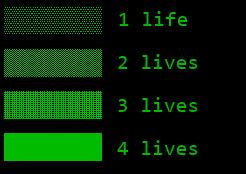
\includegraphics[scale=1]{figs/brikker.png}
\caption{Brikker med forskelligt antal liv tegnes forskelligt}
\label{fig:brikker}
\end{figure}
%\begin{itemize}
\item \textbf{Baner gemt i et array i ROM'en.} Vi har valgt at hardcode brikkernes bredde og højde for at spare plads når vi gemmer banerne i ROM'en. På denne måde kan en bane i ROM'en gemmes i arrayet\\ \texttt{unsigned char rom levels[4][BRICK\_TABLE\_HEIGHT][BRICK\_TABLE\_WIDTH]}. Dette arrray er et tredimensionalt array af chars der er gemt i ROM'en. Det indeholder fire "lag" der hver indeholder de todimensionale data til en bane. Værdien af hver char er antallet af liv den tilsvarende brik får. Når banen initialiseres, løbes dette array og arrayet \texttt{bricks[][]} igennem og brikkerne i \texttt{bricks[][]} får det antal liv der står i \texttt{levels[][][]} arrayet. Den dynamiske hukommelse i mikroprocessoren indeholder således kun et array af brikker der svarer til den aktuelle bane. Et eksempel på hvordan en bane er gemt i arrayet \texttt{levels[n][][]} er vist nedenfor. 
\begin{lstlisting}
	{
		{ 0, 0, 0, 0, 0, 0, 0, 0, 0, 0, 0, 0, 0, 0 },
		{ 0, 0, 0, 0, 0, 0, 0, 0, 0, 0, 0, 0, 0, 0 },
		{ 0, 0, 0, 0, 0, 0, 0, 0, 0, 0, 0, 0, 0, 0 },
		{ 0, 0, 0, 0, 0, 0, 0, 0, 0, 0, 0, 0, 0, 0 },
		{ 0, 0, 0, 0, 0, 0, 0, 0, 0, 0, 0, 0, 0, 0 },
		{ 0, 0, 0, 0, 0, 0, 0, 0, 0, 0, 0, 0, 0, 0 },
		{ 0, 1, 1, 1, 1, 1, 1, 1, 1, 1, 1, 1, 1, 0 },
		{ 0, 1, 1, 1, 1, 1, 1, 1, 1, 1, 1, 1, 1, 0 },
		{ 0, 2, 2, 2, 2, 2, 2, 2, 2, 2, 2, 2, 2, 0 },
		{ 0, 3, 3, 3, 3, 3, 3, 3, 3, 3, 3, 3, 3, 0 },
		{ 0, 4, 4, 4, 4, 4, 4, 4, 4, 4, 4, 4, 4, 0 },
		{ 0, 0, 0, 0, 0, 0, 0, 0, 0, 0, 0, 0, 0, 0 },
		{ 0, 0, 0, 0, 0, 0, 0, 0, 0, 0, 0, 0, 0, 0 },
		{ 0, 0, 0, 0, 0, 0, 0, 0, 0, 0, 0, 0, 0, 0 },
		{ 0, 0, 0, 0, 0, 0, 0, 0, 0, 0, 0, 0, 0, 0 },
		{ 0, 0, 0, 0, 0, 0, 0, 0, 0, 0, 0, 0, 0, 0 },
		{ 0, 0, 0, 0, 0, 0, 0, 0, 0, 0, 0, 0, 0, 0 },
		{ 0, 0, 0, 0, 0, 0, 0, 0, 0, 0, 0, 0, 0, 0 },
		{ 0, 0, 0, 0, 0, 0, 0, 0, 0, 0, 0, 0, 0, 0 },
	},
\end{lstlisting}
Banen der svarer til det ovenstående array, er vist på Figur \ref{fig:level1}. 

\begin{figure}[h!]
\centering
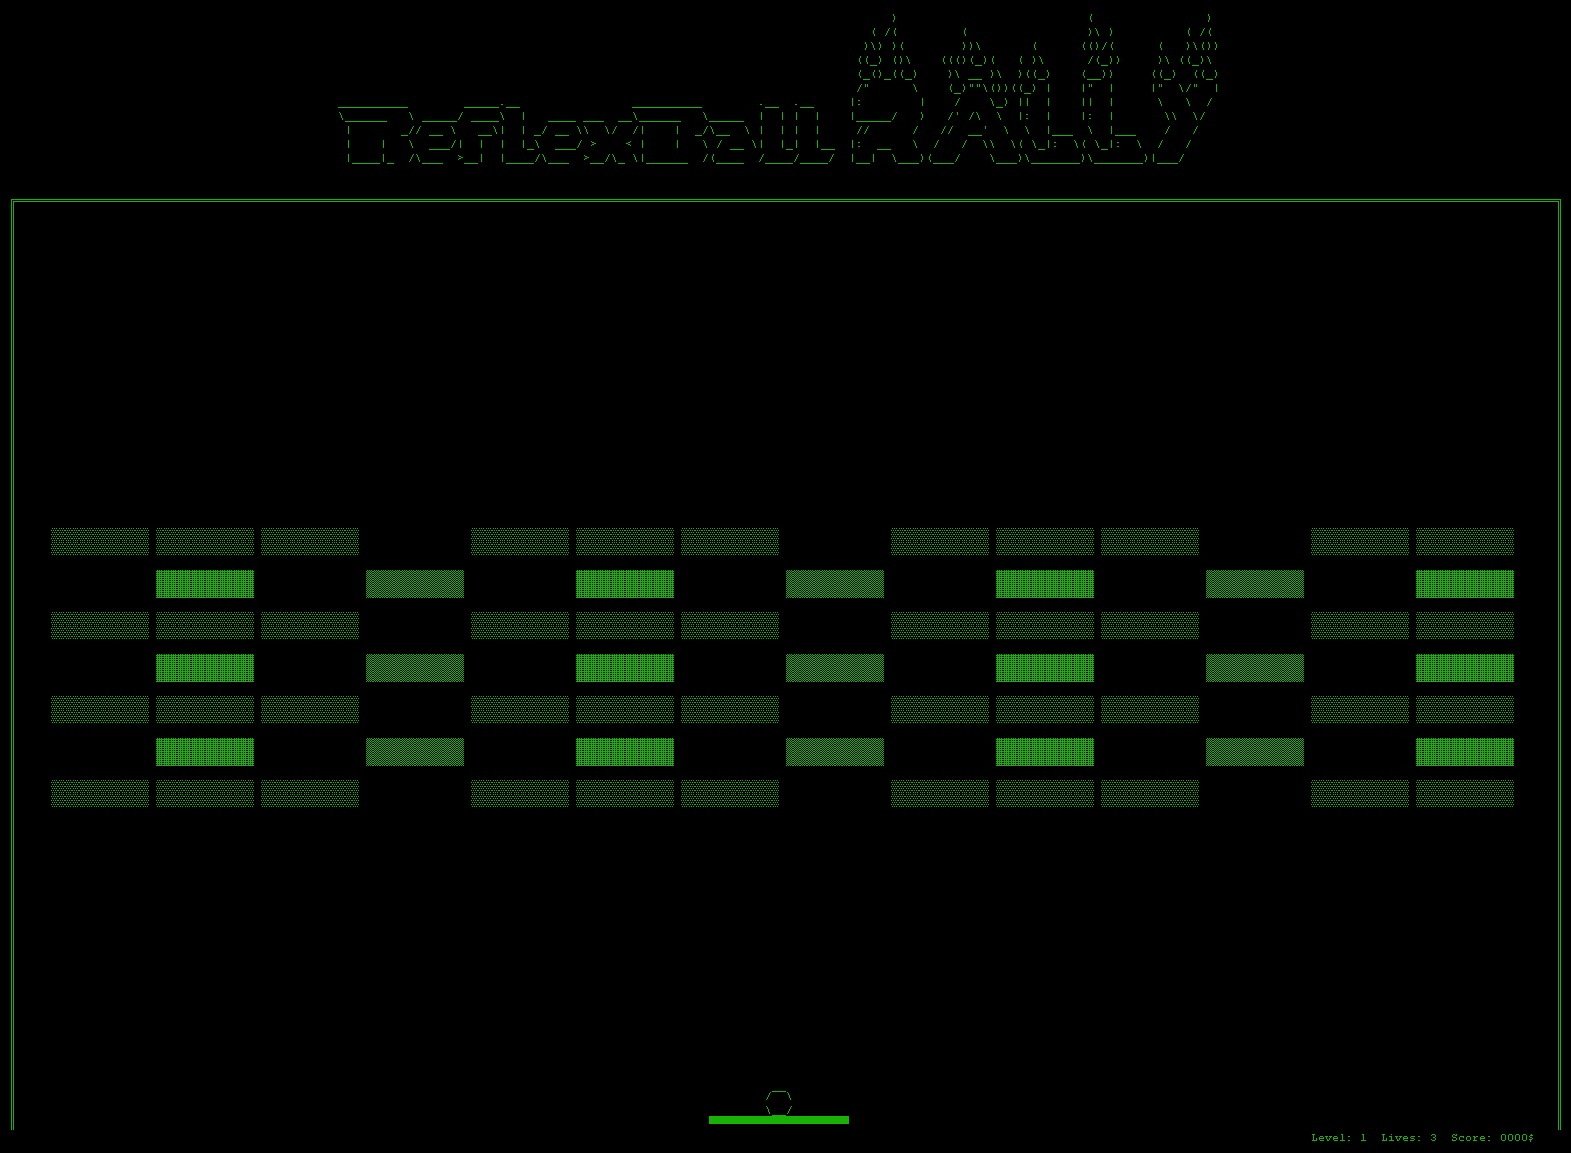
\includegraphics[scale=0.25]{figs/screenshots/level1.png}
\caption{Level 1 i spillet}
\label{fig:level1}
\end{figure}

%\end{itemize}
\item \textbf{Tjekke om man rammer brikker.} Den helt store udfordring med brikkerne var at tjekke om bolden ramte dem. Ved hver eneste iteration af spillet gennemløber vi arrayet \texttt{bricks[][]} og for alle brikker med mere end 0 liv tjekker vi om bolden har ramt og i givet fald hvordan.\\
Når spillet itereres og bolden flyttes tjekker vi først om bolden rammer brikkerne før vi tegner den. Hvis bolden har ramt en brik reflekteres den og får sin nye position før den tegnes. Hvis bolden har ramt en brik, er boldens koordinater altså inde i brikken når vi tjekker.

For at bolden skulle bevæge sig lige hurtigt i begge retninger på skærmen har vi lavet x-komposanten af boldens vektor dobbelt så stor. Det giver nogle ekstra udfordringer når bolden rammer brikkerne. Når bolden kan bevæge sig 2 karakterer i x-retningen kan den ramme brikkerne fra siden på en række forskellige måder. Disse er vist for højre side af brikken på Figur \ref{fig:SideReflexSamlet}. 
Når vi har itereret spillet og tjekker boldens position kan den på x-aksen befinde sig både en eller to karakterer inde i brikken. Den kan således ramme brikken på seks forskellige måder som vist på ovennævnte figur. Det er vigtigt at tage højde for at bolden kan ramme to karakterer ind i brikken når man tjekker om bolden har ramt brikken for siden i midten. Hvis man ikke tager højde for dette, vil bolden bevæge sig igennem brikken mens den reflekteres af toppe og bunden. 

\begin{figure}[h!]
\centering
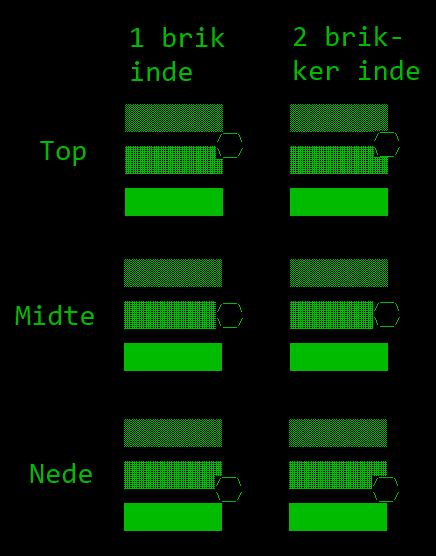
\includegraphics[scale=0.75]{figs/side_reflex_samlet.png}
\caption{Forskellige måder bolden kan ramme fra siden}
\label{fig:SideReflexSamlet}
\end{figure}


For at give et godt gameplay har vi besluttet at bolden fortrinsvis skal reflekteres ned og op så brugeren kan få den. Dette er vist på Figur \ref{fig:ReflexOppeFri}. Når bolden rammer brikken fra toppen og er 2 karakterer inde i brikken vil den blive reflekteret som vist på figuren. Hvis bolden havde ramt på samme måde, men var kommet nedefra var den blevet reflekteret som om den havde ramt siden af brikken.

Det der er vist på denne figur er, borset fra de omgivende brikker, samme situation som på Figur \ref{fig:SideReflexSamlet}, Top, 2 brikker inde. 

 
\begin{figure}[h!]
\centering
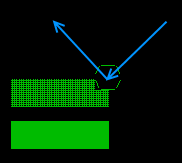
\includegraphics[scale=1]{figs/reflex_oppe_fri.png}
\caption{Forskellige måder bolden kan ramme fra siden}
\label{fig:ReflexOppeFri}
\end{figure}



\begin{itemize}
\item Højre/venstre og oppe/nede
\item Kanter?
\end{itemize}
\item Trække liv fra brikkerne
\item Lave deflect på baggrund af om der er brikker omkring brikken
\begin{itemize}
\item Forklare tilfældene med at ramme to brikker af gangen
\item Forklare tilfældene med at ramme flere hjørner
\end{itemize}
\item Briklogik korrigeret fordi der bevæges 2 karakterer i x-retningen
\end{itemize}

\subsection{Flowchart for briklogikken}

\newpage

% Flowcharting techniques for easy maintenance
% Author: Brent Longborough
% =================================================
% Set up a few colours
\colorlet{lcfree}{Green3}
\colorlet{lcnorm}{Blue3}
\colorlet{lccong}{Red3}
% -------------------------------------------------
% Set up a new layer for the debugging marks, and make sure it is on
% top
\pgfdeclarelayer{marx}
\pgfsetlayers{main,marx}
% A macro for marking coordinates (specific to the coordinate naming
% scheme used here). Swap the following 2 definitions to deactivate
% marks.
\providecommand{\cmark}[2][]{%
  \begin{pgfonlayer}{marx}
    \node [nmark] at (c#2#1) {#2};
  \end{pgfonlayer}{marx}
  } 
\providecommand{\cmark}[2][]{\relax} 
% -------------------------------------------------
% Start the picture
\begin{center}
\newgeometry{margin=1cm}
\begin{tikzpicture}[%
    >=triangle 60,              % Nice arrows; your taste may be different
    start chain=going below,    % General flow is top-to-bottom
    node distance=4mm and 40mm, % Global setup of box spacing
    every join/.style={norm},   % Default linetype for connecting boxes
    ]
% ------------------------------------------------- 
% A few box styles 

% <on chain> *and* <on grid> reduce the need for manual relative
% positioning of nodes
\tikzset{
  base/.style={draw, on chain, on grid, align=center, minimum height=2ex},
  proc/.style={base, rectangle, fill=blue!20, font={\tiny}},
  test/.style={base, diamond, aspect=2.2, fill=orange!20, font={\tiny}},
  term/.style={proc, rounded corners,fill=green!20, font={\tiny}},
  placeholder/.style={base, on chain, text width=6em, fill=white, font={\tiny}},
  % coord node style is used for placing corners of connecting lines
  coord/.style={coordinate, on chain, on grid, node distance=4mm and 4mm},
  % nmark node style is used for coordinate debugging marks
  nmark/.style={draw, cyan, circle, font={\sffamily\bfseries}},
  % -------------------------------------------------
  % Connector line styles for different parts of the diagram
  norm/.style={->, draw, lcnorm},
  free/.style={->, draw, lcfree},
  cong/.style={->, draw, lccong},
  it/.style={font={\tiny}}
}
% -------------------------------------------------
% Start by placing the nodes
\node [proc, it] (p0) {Iterate ball};
\node [test, join] (t0) {Indenfor bane?};

% No join for exits from test nodes - connections have more complex
% requirements
% We continue until all the blocks are positioned
\node [proc, fill=lcfree!25,] (p1) {For(alle brikker)};
\node [test, join]	(t1)	{Ramt brik?};
\node [term]    	(p2) 	{score++};
\node [test, join]	(t2) 	{Top/bund?};
\node [test] 		(t3)	{DeflectedY?};
\node [test] 		(t4) 	{Top, ven- \\ stre/højre?};
\node [test] 		(t5)	{Brik over?};
\node [term]  		(p3)    {dontDeflectY};

\node [placeholder, color=white, frame=none, fill=white] ;
\node [placeholder, color=white, frame=none, fill=white] ;
\node [placeholder, color=white, frame=none, fill=white] ;
\node [placeholder, color=white, frame=none, fill=white] ;
\node [placeholder, color=white, frame=none, fill=white] ;

\node [test]		(t8)  {Ramt midt \\ i brikken?};
\node [term]  		(p5)  {dontDeflectY};
\node [test, join]	(t9)  {Top fra neden?};
\node [term]		(p6)	  {dontDeflectY};


\node [test, join]	(t11)		{dontDeflectY?};\\
\node [proc, it] 	(p8) 		{Reflekter Y};


% We position the next block explicitly as the first block in the
% second column.  The chain 'comes along with us'. The distance
% between columns has already been defined, so we don't need to
% specify it.
%%%% NÆSTE KOLONNE
\node [placeholder, color=white, frame=none, fill=white, right=of t0] (k0) {kan den have tekst?};


\node [placeholder, color=white, frame=none, fill=white, right=of t4]  {kan den have tekst?};
\node [test] 	(t6) {Bund, ven- \\ stre/højre?};
\node [test]				(t7) {Brik under?};
\node [term]      	  		(p4) {dontDeflectY};

\node [test, right=of t9] 	(t10)  	{Bund fra oven?};
\node [term]      			(p7)	{dontDeflectY};


%%%% NÆSTE KOLONNE
\node [test, right=of k0] 	(t12) {Side? \& !xDeflected};
\node [test] 				(t13) {Top/bund?};
\node [test] 				(t14) {Venstre \& \\ brik til venstre?};
%\node [test] (t14) {Levende brik til venstre?};
\node [term] 				(p9)  {dontDeflectX};
\node [test, join] 			(t15) {Højre side \& \\ brik til højre?};
%\node [test] (t16) {Levende brik til højre?};
\node [term]      			(p10)  {dontDeflectX};


\node [test, join] 	(t16) {Venstre side?};
\node [test] 		(t17) {Kommer fra \\ højre?};
\node [term]      	(p11) {dontDeflectX};
% Tre til højre for som er under i hieraki

\node [test] 	(t20) {Fra siden, \\ ml. top og bund?};
\node [test] 		(t21) {Top?};
\node [test] 		(t22) {Fra oven \& \\ frit over?};
\node [term]      	(p13) {dontDeflectX};
\node [test, join] 	(t24) {dontDeflectX?};
\node [proc, it] 	(p15) {Reflekter X};


%%\node [test] (t19) {Højre side?};
%%%%% NÆSTE KOLONNE
\node [placeholder, color=white, frame=none, right=of t12] (k1) {kan den have tekst?};
\node [test, right=of t16] 	(t18) {Højre side?};
\node [test] 				(t19) {Kommer fra \\ venstre?};
\node [term]      			(p12) {dontDeflectX};

\node [test, right=of t22] 	(t23) {Fra neden \& \\ frit under?};
\node [term]    			(p14) {dontDeflectX};

%%%%% NÆSTE KOLONNE
\node [test, right=of k1] 	(t25) {Under striker?};
\node [test] 				(t26) {gameStarted?};
\node [test] 				(t27) {Udenfor sider?};
\node [proc, it] 			(p16) {Reflekter X};
\node [test, join]			(t28) {Over top/ \\ på striker?};
\node [test] 				(t29) {Ramt striker?};
\node [proc] 				(p17) {Roter afhængigt \\ af hvor man rammer};
\node [proc, join] 			(p18) {Reflekter Y};
\node [proc, join] 			(p19) {drawBigBall};






% -------------------------------------------------
% Now we place the coordinate nodes for the connectors with angles, or
% with annotations. We also mark them for debugging.
%\node [coord, right=of t1] (c1)  {}; %\cmark{1}   
%\node [coord, right=of t3] (c3)  {}; %\cmark{3}   
%\node [coord, right=of t6] (c6)  {}; %\cmark{6}   
%\node [coord, right=of t7] (c7)  {}; %\cmark{7}   
%\node [coord, left=of t4]  (c4)  {}; %\cmark{4}   
%\node [coord, right=of t4] (c4r) {}; %\cmark[r]{4}
%\node [coord, left=of t7]  (c5)  {}; %\cmark{5} 

% -------------------------------------------------

% -------------------------------------------------
% All the other connections come out of tests and need annotating
% First, the straight north-south connections. In each case, we first
% draw a path with a (consistently positioned) annotation node, then
% we draw the arrow itself.
\path (t0.south) to node [near start, xshift=1em] {$ja$} (p1);
  \draw [->,lcnorm] (t0.south) -- (p1);
 
\path (t1.south) to node [near start, xshift=1em] {$ja$} (p2);
  \draw [->,lcnorm] (t1.south) -- (p2);
  
\path (t2.south) to node [near start, xshift=1em] {$ja$} (t3);
  \draw [->,lcnorm] (t2.south) -- (t3);  

\path (t3.south) to node [near start, xshift=1em] {$nej$} (t4);
  \draw [->,lcnorm] (t3.south) -- (t4);
  
\path (t4.south) to node [near start, xshift=1em] {$ja$} (t5);
  \draw [->,lcnorm] (t4.south) -- (t5);

\path (t5.south) to node [near start, xshift=1em] {$ja$} (p3);
  \draw [->,lcnorm] (t5.south) -- (p3); 

\path (t8.south) to node [near start, xshift=1em] {$ja$} (p5);
  \draw [->,lcnorm] (t8.south) -- (p5);
  
\path (t9.south) to node [near start, xshift=1em] {$ja$} (p6);
  \draw [->,lcnorm] (t9.south) -- (p6); 
  
\path (t11.south) to node [near start, xshift=1em] {$nej$} (p8);
  \draw [->,lcnorm] (t11.south) -- (p8);
  
%%Næste række (mellemrække)
\path (t6.south) to node [near start, xshift=1em] {$ja$} (t7);
  \draw [->,lcnorm] (t6.south) -- (t7);
 
\path (t7.south) to node [near start, xshift=1em] {$ja$} (p4);
  \draw [->,lcnorm] (t7.south) -- (p4);
  
\path (t10.south) to node [near start, xshift=1em] {$ja$} (p7);
  \draw [->,lcnorm] (t10.south) -- (p7);

%%Næste række
\path (t12.south) to node [near start, xshift=1em] {$ja$} (t13);
  \draw [->,lcnorm] (t12.south) -- (t13); 
  
\path (t13.south) to node [near start, xshift=1em] {$ja$} (t14);
  \draw [->,lcnorm] (t13.south) -- (t14);

\path (t14.south) to node [near start, xshift=1em] {$ja$} (p9);
  \draw [->,lcnorm] (t14.south) -- (p9); 

\path (t15.south) to node [near start, xshift=1em] {$ja$} (p10);
  \draw [->,lcnorm] (t15.south) -- (p10); 

\path (t16.south) to node [near start, xshift=1em] {$ja$} (t17);
  \draw [->,lcnorm] (t16.south) -- (t17); 

\path (t17.south) to node [near start, xshift=1em] {$ja$} (p11);
  \draw [->,lcnorm] (t17.south) -- (p11);

\path (t20.south) to node [near start, xshift=1em] {$ja$} (t21);
  \draw [->,lcnorm] (t20.south) -- (t21);
  
\path (t21.south) to node [near start, xshift=1em] {$ja$} (t22);
  \draw [->,lcnorm] (t21.south) -- (t22);  

\path (t22.south) to node [near start, xshift=1em] {$ja$} (p13);
  \draw [->,lcnorm] (t22.south) -- (p13);

\path (t24.south) to node [near start, xshift=1em] {$nej$} (p15);
  \draw [->,lcnorm] (t24.south) -- (p15);
  

% Næste række (mellemrække)
\path (t18.south) to node [near start, xshift=1em] {$ja$} (t19);
  \draw [->,lcnorm] (t18.south) -- (t19);

\path (t19.south) to node [near start, xshift=1em] {$ja$} (p12);
  \draw [->,lcnorm] (t19.south) -- (p12);

\path (t23.south) to node [near start, xshift=1em] {$ja$} (p14);
  \draw [->,lcnorm] (t23.south) -- (p14);


% Næste række
\path (t25.south) to node [near start, xshift=1em] {$nej$} (t26);
  \draw [->,lcnorm] (t25.south) -- (t26);

\path (t26.south) to node [near start, xshift=1em] {$ja$} (t27);
  \draw [->,lcnorm] (t26.south) -- (t27);
  
\path (t27.south) to node [near start, xshift=1em] {$ja$} (p16);
  \draw [->,lcnorm] (t27.south) -- (p16);
  
\path (t28.south) to node [near start, xshift=1em] {$ja$} (t29);
  \draw [->,lcnorm] (t28.south) -- (t29);
  
\path (t29.south) to node [near start, xshift=1em] {$ja$} (p17);
  \draw [->,lcnorm] (t29.south) -- (p17);




%\path (t6.south) to node [near start, xshift=1em] {$y$} (t7); 
% \draw [*->,lcfree] (t6.south) -- (t7); 
% ------------------------------------------------- 
% Now the straight east-west connections. To provide consistent
% positioning of the test exit annotations, we have positioned
% coordinates for the vertical part of the connectors. The annotation
% text is positioned on a path to the coordinate, and then the whole
% connector is drawn to its destination box.
%\path (t3.east) to node [near start, yshift=1em] {$n$} (c3); 
%  \draw [o->,lccong] (t3.east) -- (p8);
%\path (t4.east) to node [yshift=-1em] {$k \leq 0$} (c4r); 
%  \draw [o->,lcnorm] (t4.east) -- (p9);

% -------------------------------------------------
% The coordinates

\node [coord, right = 20mm of p1] (cp1)  {}; %\cmark{1}
\node [coord, right = 20mm of t1] (ct1)  {}; %\cmark{1}     

% -------------------------------------------------
% Finally, the twisty connectors. Again, we place the annotation
% first, then draw the connector


\path (t1.east) to node [very near start, yshift=1em] {$nej$} (ct1); 
  \draw [->,lcnorm] (t1.east) -| (cp1) --(p1);

%\path (t1.east) to node [near start, yshift=1em] {$n$} (c1); 
%  \draw [o->,lcfree] (t1.east) -- (c1) |- (p4);
%\path (t2.east) -| node [very near start, yshift=1em] {$n$} (c1); 
%  \draw [o->,lcfree] (t2.east) -| (c1);
%\path (t4.west) to node [yshift=-1em] {$k>0$} (c4); 
%  \draw [*->,lcnorm] (t4.west) -- (c4) |- (p3);
%\path (t5.east) -| node [very near start, yshift=1em] {$n$} (c6); 
%  \draw [o->,lcfree] (t5.east) -| (c6); 
%\path (t6.east) to node [near start, yshift=1em] {$n$} (c6); 
%  \draw [o->,lcfree] (t6.east) -| (c7); 
%\path (t7.east) to node [yshift=-1em] {$k \leq 0$} (c7); 
%  \draw [o->,lcfree] (t7.east) -- (c7)  |- (p9);
%\path (t7.west) to node [yshift=-1em] {$k>0$} (c5); 
%  \draw [*->,lcfree] (t7.west) -- (c5) |- (p5);
% -------------------------------------------------
% A last flourish which breaks all the rules
%\draw [->,MediumPurple4, dotted, thick, shorten >=1mm]
%  (p9.south) -- ++(5mm,-3mm)  -- ++(27mm,0) 
%  |- node [black, near end, yshift=0.75em, it]
%   {(When message + resources available)} (p0);
% -------------------------------------------------
\end{tikzpicture}
\restoregeometry
\end{center}


		\chapter{Brugermanual}

I dette afsnit vil vi beskrive en simpel brugermanual til spillet. Vi vil fokusere på den primære styringsmetode vha. rattet og gearstangen. Spillet kan dog også spillet vha. computerens keyboard eller knapperne på udviklings boardet.
\\

Det første der møder en når man starter spillet er skærmbilledet der ses på figur \ref{fig:startup}. Den blinkende tekst under logoet angiver at brugeren skal trykke på en valgfri tast for at starte spillet. ASCII arten af rattet skulle gerne give en indikation af hvordan spillet styres. Et billede af rattet til sammenligning kan ses i figur \ref{fig:rat_med_controls}.

\begin{figure}[h!]
\begin{minipage}[b]{0.49\textwidth}

\includegraphics[width=\linewidth]{figs/screenshots/startup_crop_ny.png}
\caption{Screenshot af startup skærmen}
\label{fig:startup}
\end{minipage}\hfill
\begin{minipage}[b]{0.49\textwidth}
\includegraphics[width=\linewidth]{figs/rat_med_controls.png}
\caption{Oversigt over styring af rattet}
\label{fig:rat_med_controls}
\end{minipage}\hfill
\end{figure}

Derefter vises menuen svarende til den i figur \ref{fig:menu_2}. Her kan brugeren vælge sværhedsgraden. Brugeren kan således flytte bolden op og ned vha. gearet. Når den ønskede sværhedsgrad er valgt kan denne vælges ved at trykke på en af de to knapper der sidder på rattet. Den valgte sværhedsgrad bestemmer derefter bredden af strikeren, samt hvor hurtigt bolden skal begynde at forøge dens hastighed. Ved valg af Chuck Norris mode er boldens hastighed dog den maksimale hastighed fra starten. For mere information henvises til funktionen \nameref{asciidisplay} i appendiks \ref{C kode}. \\

\begin{figure}[h!]
\centering
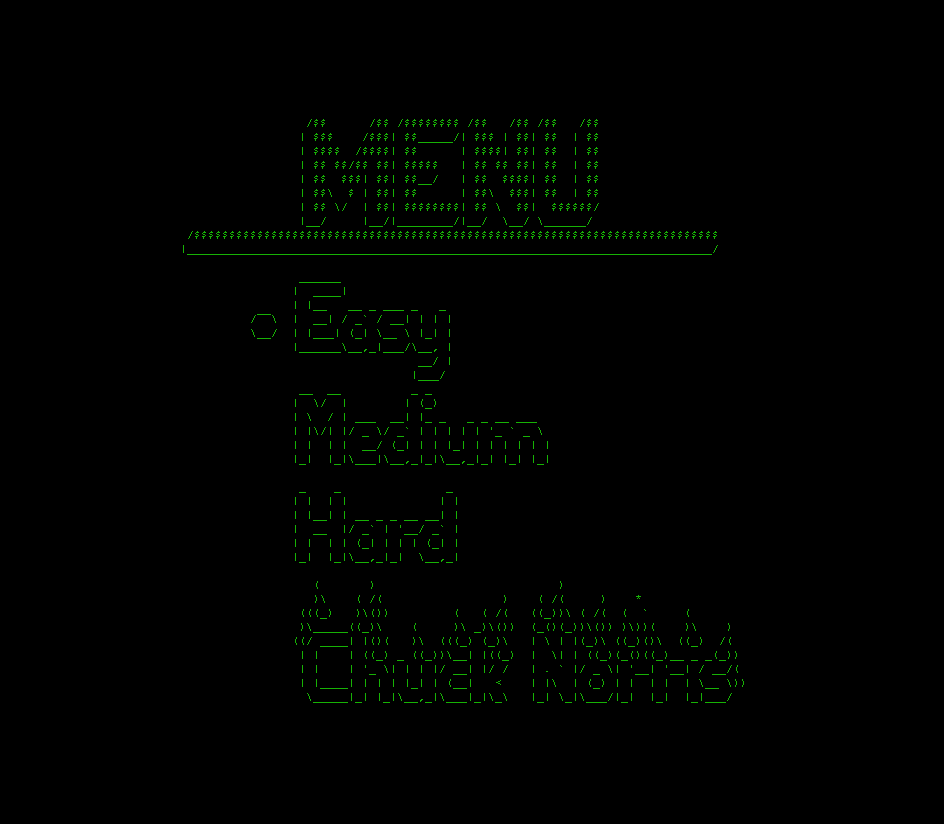
\includegraphics[scale=0.25]{figs/screenshots/menu_crop.png}
\caption{Screenshot af menuen}
\label{fig:menu_2}
\end{figure}

Efter dette begynder selve spillet. Man skyder bolden afsted ved enten af at hive gearet tilbage eller trykke på en af de to knapper på rattet. Bolden vil da skydes afsted med en vinkel på 45-135 grader. Herefter gælder det blot om at skyde alle brikkerne ned ved at bevæge strikeren ved at dreje på rattet. Hvis brugeren skyder alle brikkerne i stykker avancerer brugeren til næste level. \\

Et overblik over alle de 6 levels i spillet kan ses på figurerne nedenfor. Bemærk at der i level 6 er en række usynlige brikker, der først kommer frem når man har ramt dem én gang. Se \nameref{levels} i appendiks \ref{C kode}. \\

\begin{figure}[h!]
\begin{minipage}[b]{0.32\textwidth}
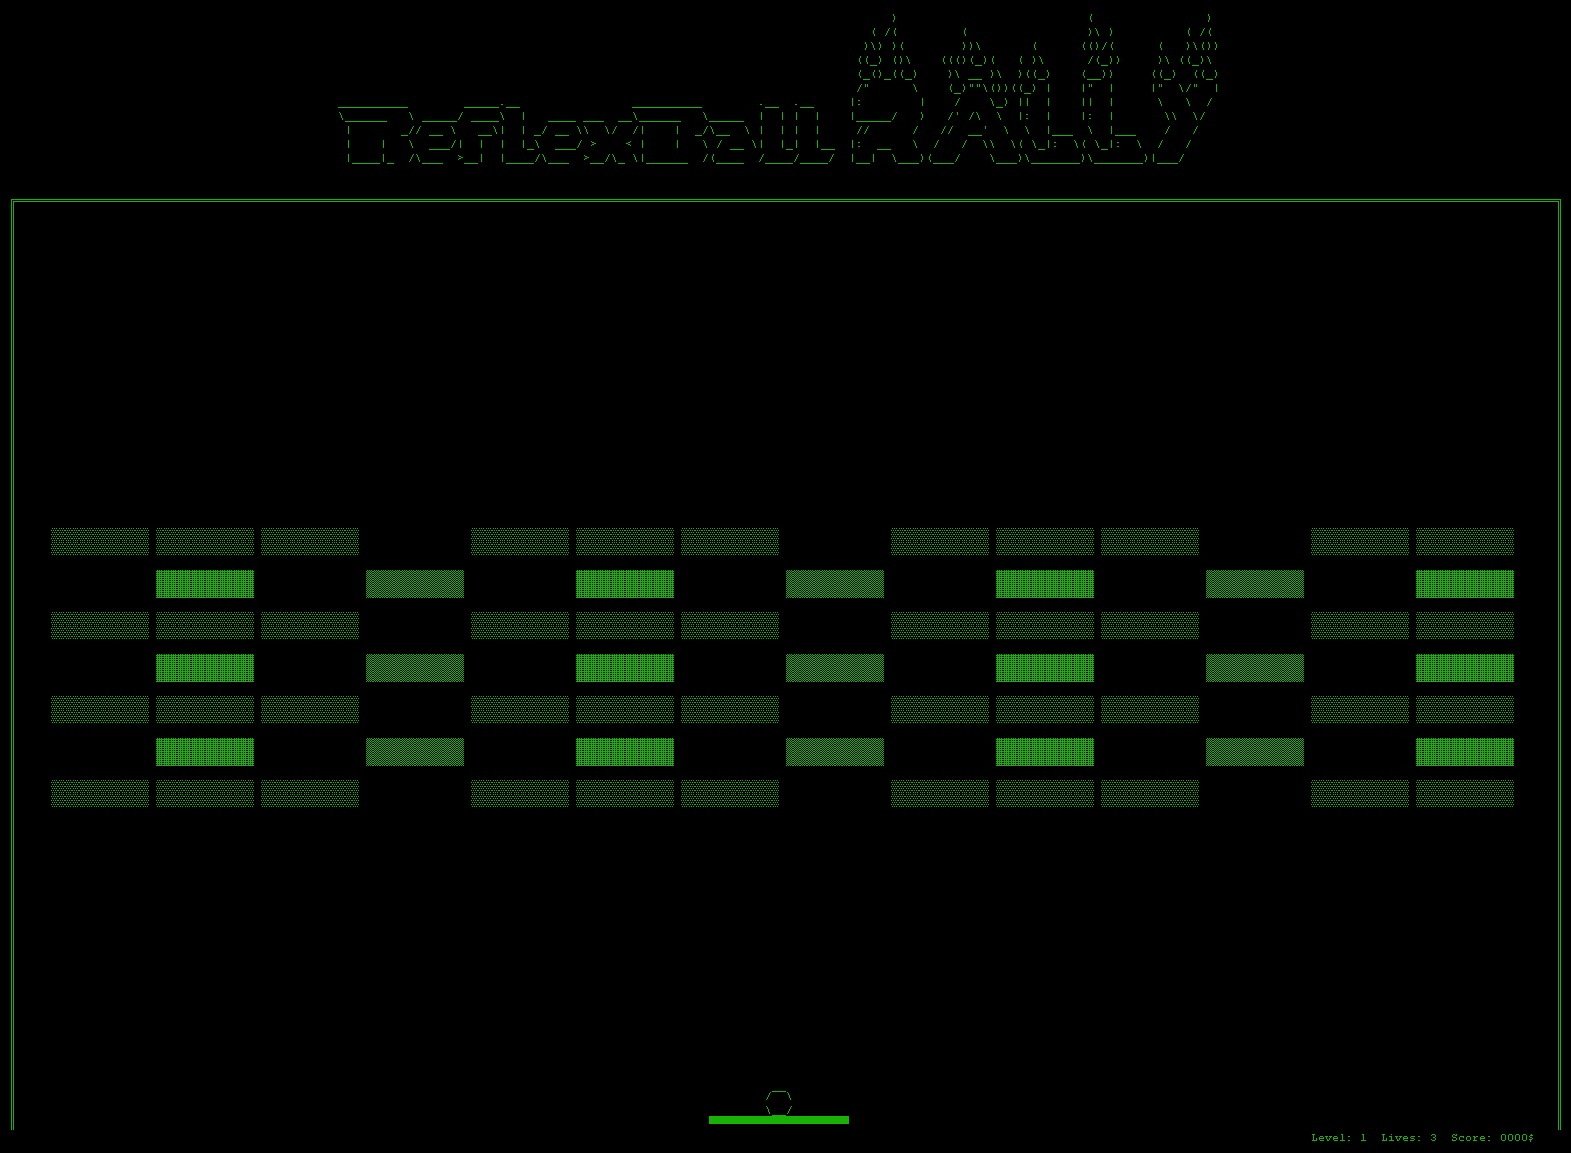
\includegraphics[width=\linewidth]{figs/screenshots/level1.png}
\caption{Level 1}
\label{fig:level1_2}
\end{minipage}\hfill
\begin{minipage}[b]{0.32\textwidth}
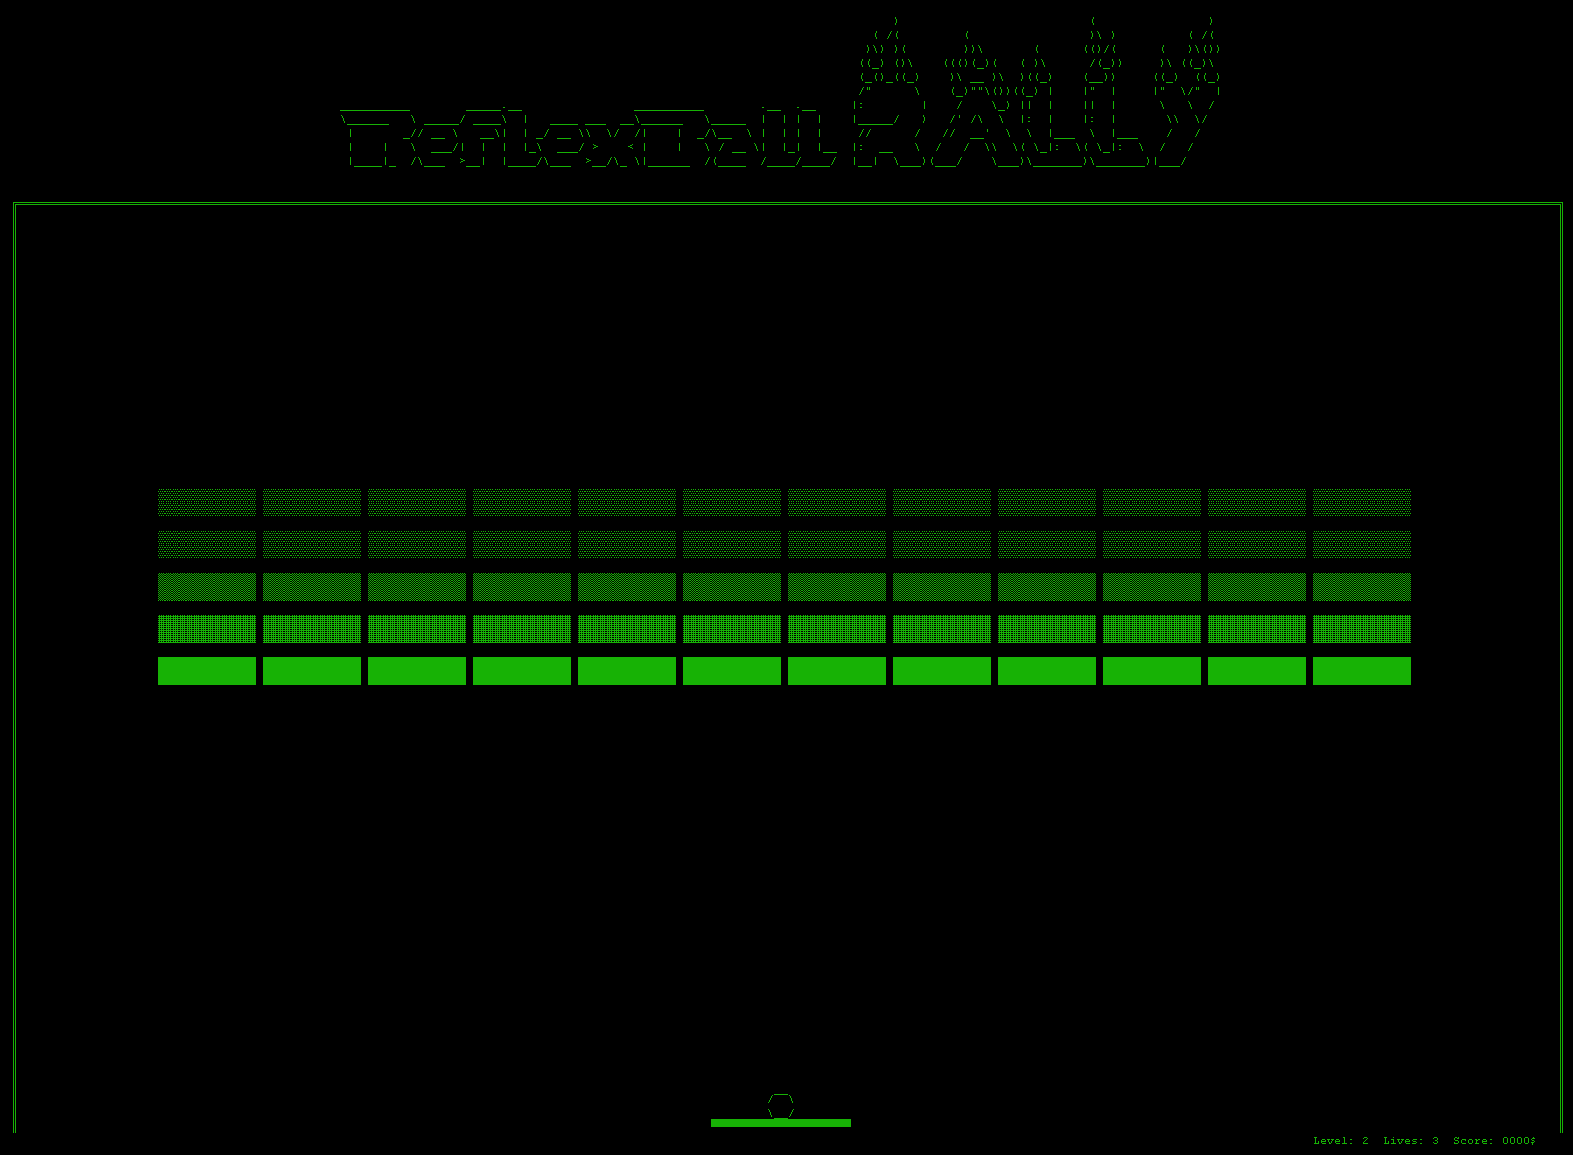
\includegraphics[width=\linewidth]{figs/screenshots/level2.png}
\caption{Level 2}
\label{fig:level2}
\end{minipage}\hfill
\begin{minipage}[b]{0.32\textwidth}
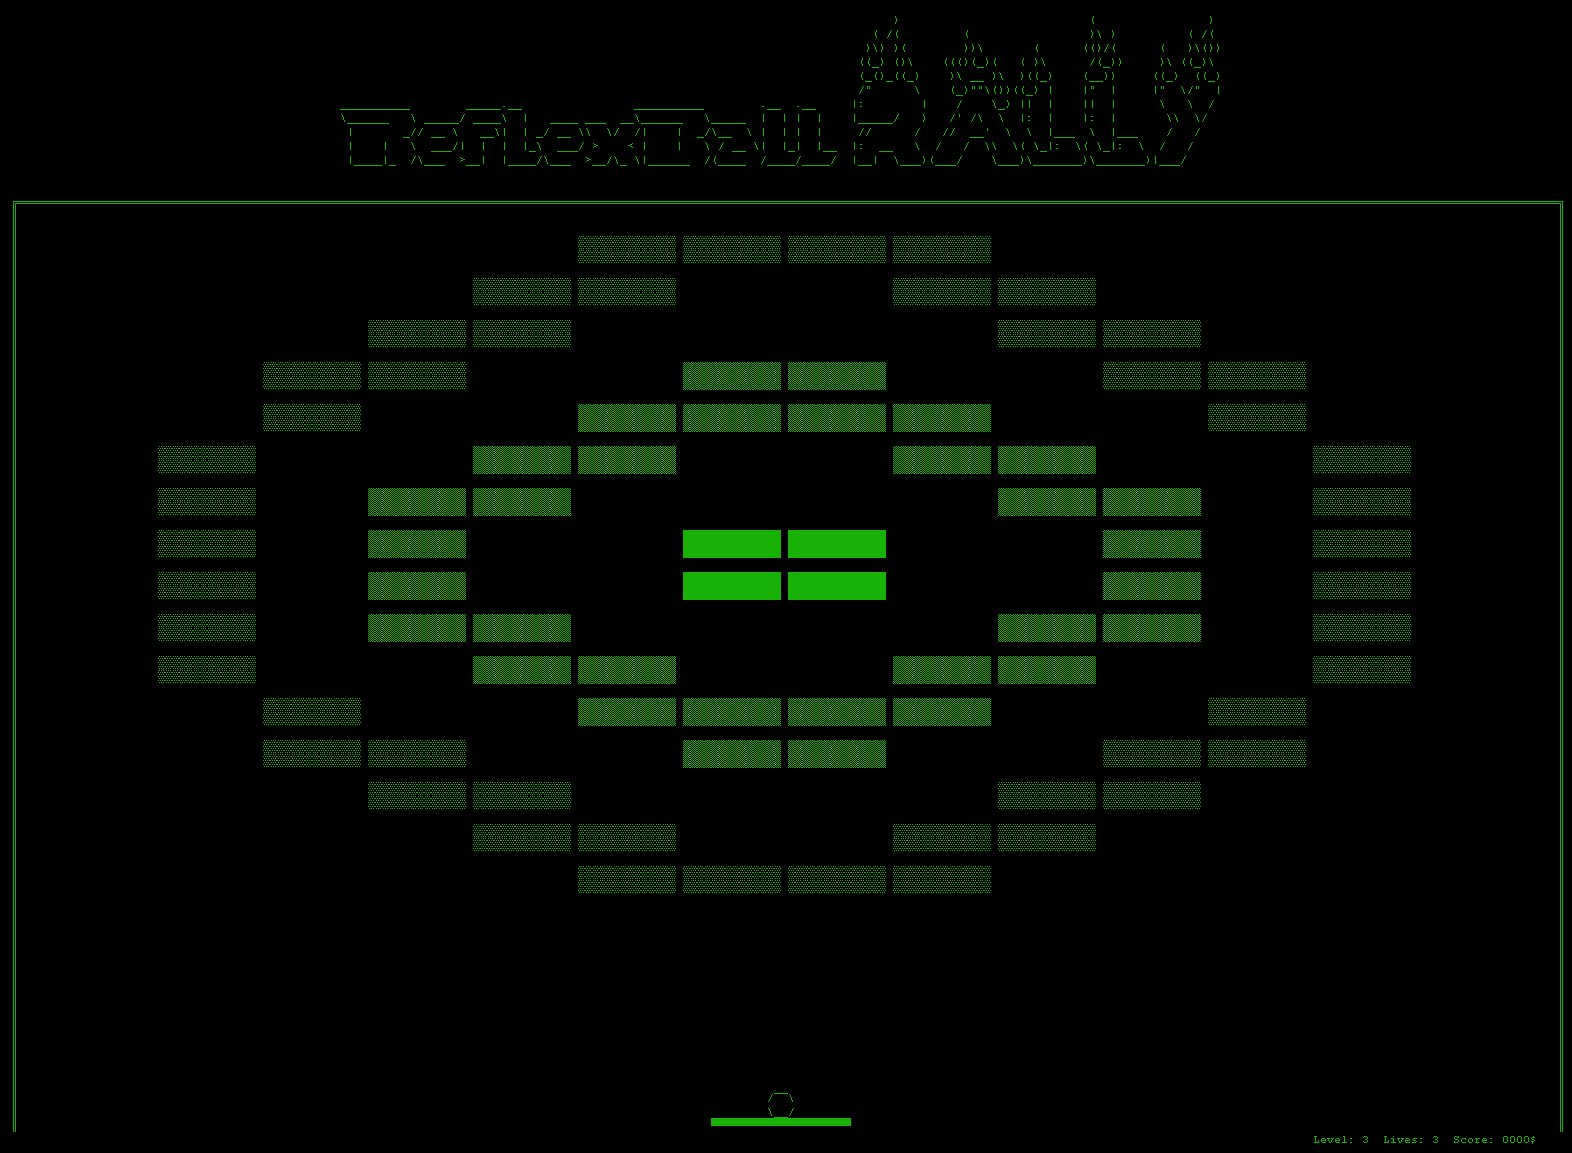
\includegraphics[width=\linewidth]{figs/screenshots/level3.png}
\caption{Level 3}
\label{fig:level3}
\end{minipage}\hfill
\begin{minipage}[b]{0.32\textwidth}
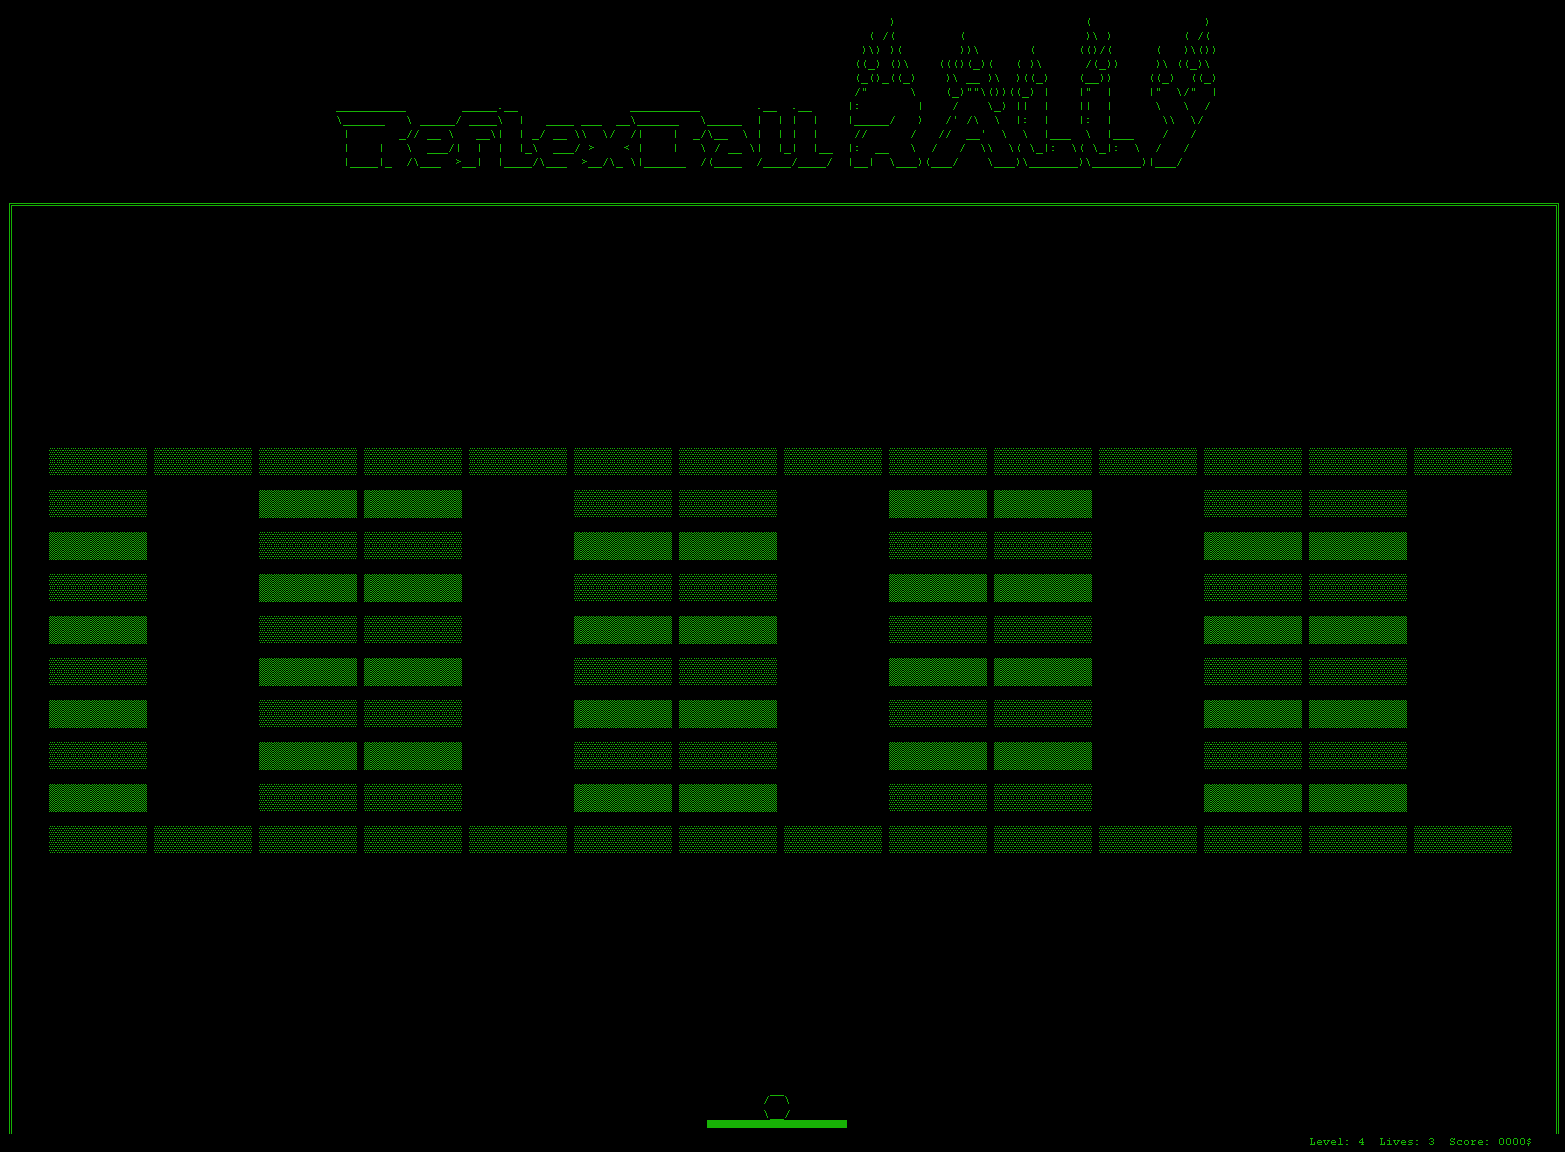
\includegraphics[width=\linewidth]{figs/screenshots/level4.png}
\caption{Level 4}
\label{fig:level4}
\end{minipage}\hfill
\begin{minipage}[b]{0.32\textwidth}
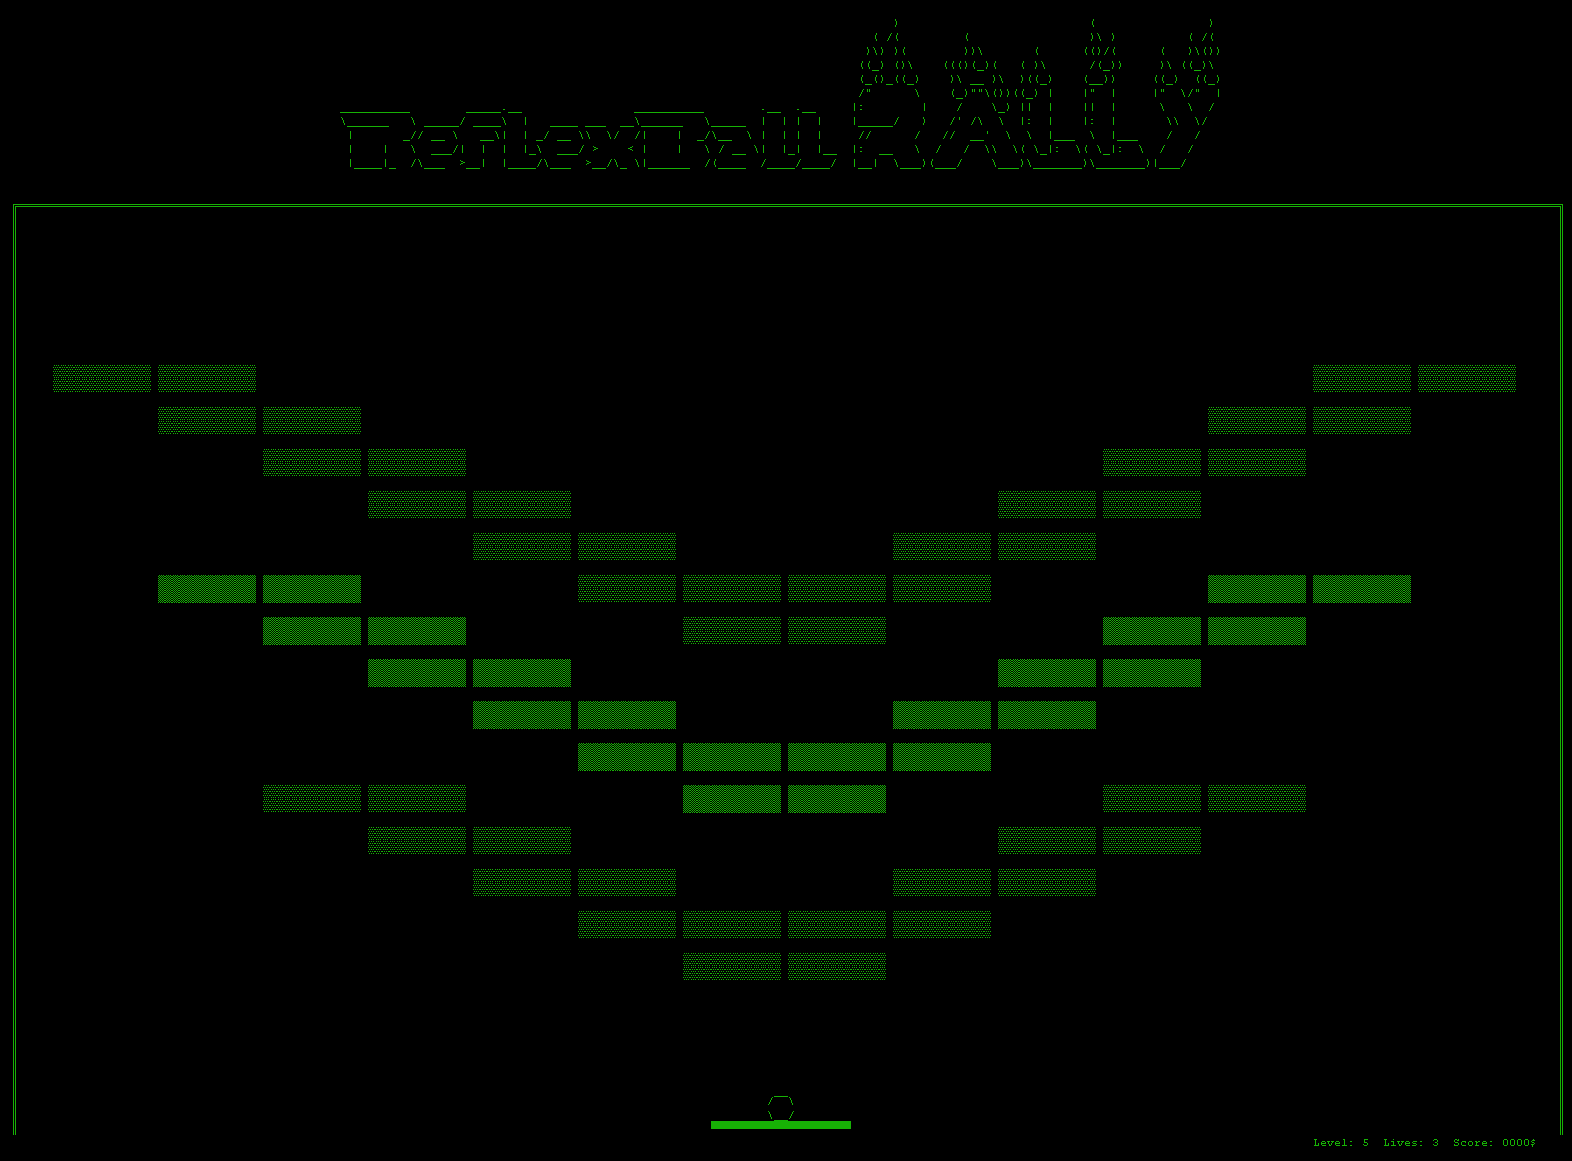
\includegraphics[width=\linewidth]{figs/screenshots/level5.png}
\caption{Level 5}
\label{fig:level5}
\end{minipage}\hfill
\begin{minipage}[b]{0.32\textwidth}
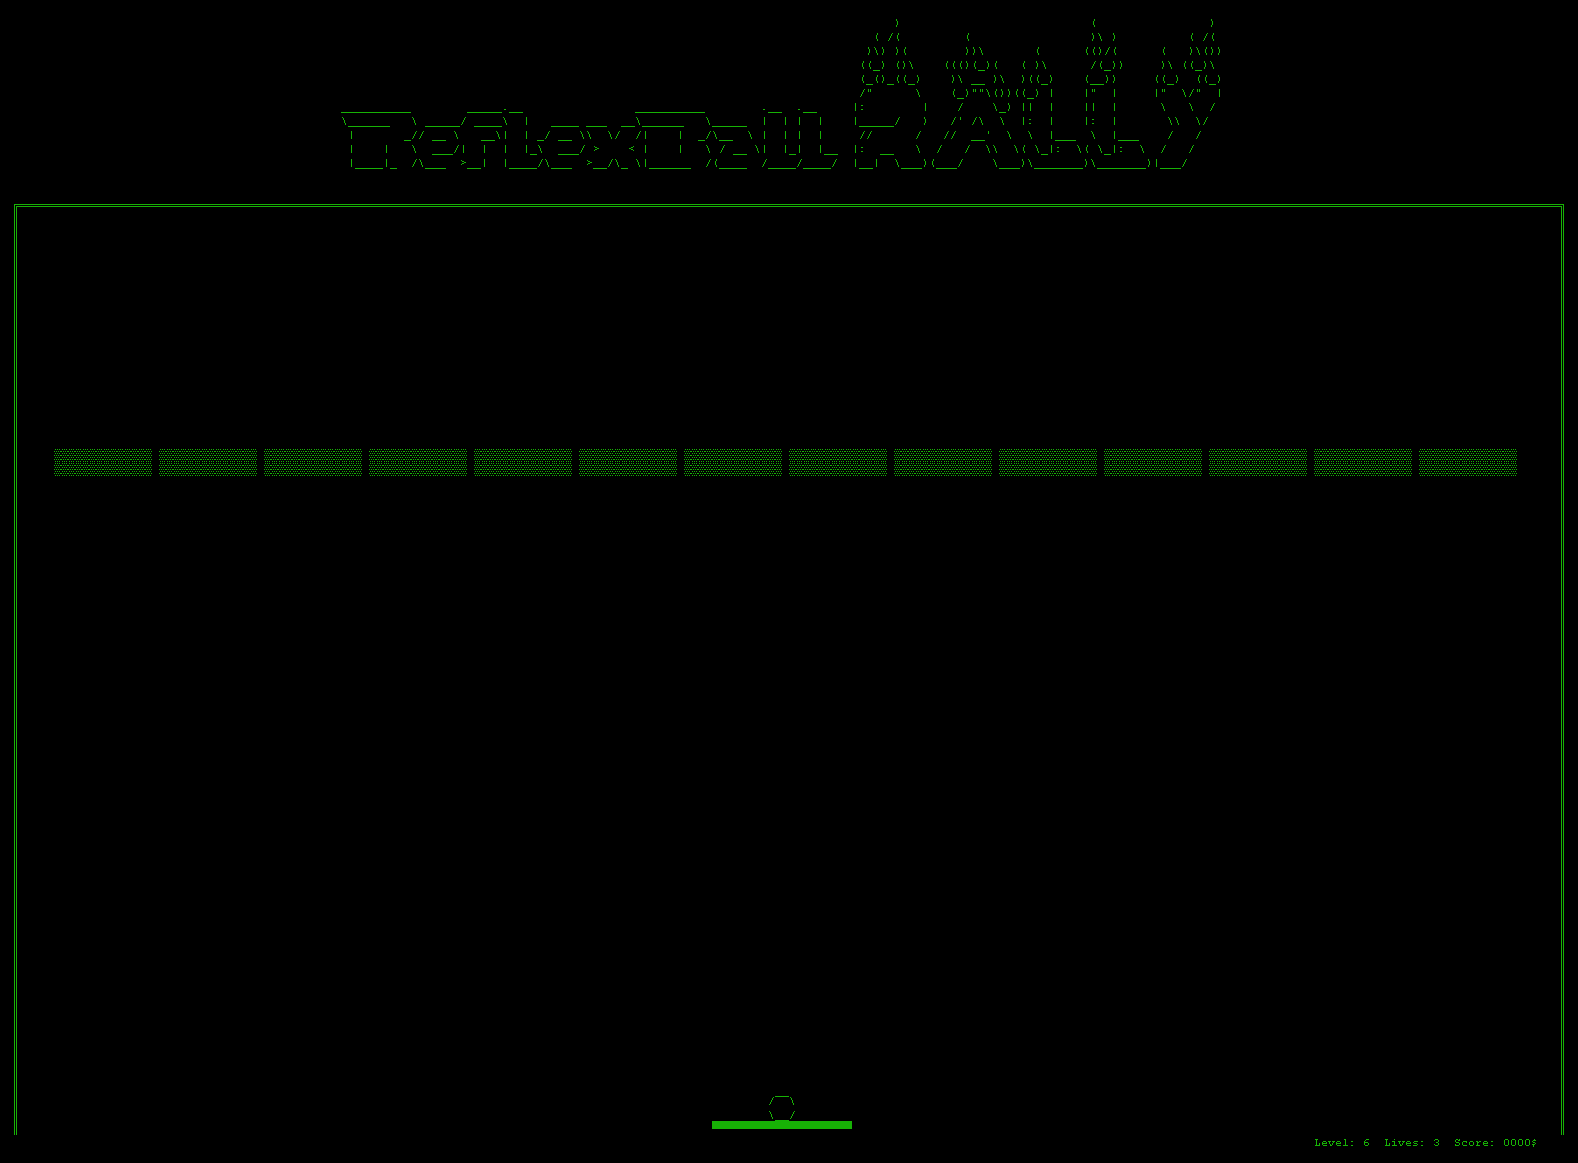
\includegraphics[width=\linewidth]{figs/screenshots/level6.png}
\caption{Level 6}
\label{fig:level6}
\end{minipage}\hfill
\end{figure}

Hvis man taber spillet vises "Game Over!" skrevet med ASCII art, samt 1 tilfældig ud af 8 forskellige undertitler. Figur \ref{fig:gameover_2} viser et screenshot af dette. \\

\begin{figure}[h!]
\centering

\includegraphics[scale=0.25]{figs/screenshots/gameover_crop.png}
\caption{Eksempel på screenshot game over tekst}
\label{fig:gameover_2}
\end{figure}

Hvis man vinder spillet på easy, medium eller hard vises et screenshot magen til figur \ref{fig:won_normal_2}, hvis man derimod vinder spillet på sværhedsgraden Chuck Norris vises et billedet som ses på figur \ref{fig:won_chuck}.

\begin{figure}[h!]
\begin{minipage}[b]{0.49\textwidth}

\includegraphics[width=\linewidth]{figs/screenshots/won_normal.png}
\caption{Screenshot ved gennemførsel af spillet}
\label{fig:won_normal_2}
\end{minipage}\hfill
\begin{minipage}[b]{0.49\textwidth}

\includegraphics[width=\linewidth]{figs/screenshots/won_chuck_crop.png}
\caption{Screenshot ved gennemførsel af spillet i Chuck Norris mode}
\label{fig:won_chuck}
\end{minipage}\hfill
\end{figure}
		\newpage
\chapter{Diskussion}

Dette projekt valgte vi at dele op i en række delmål. Delmålene var delt op i grupperne Basics, Advanced, Brikker, Helhedsindtryk og Hardware. Basics var det der skulle til for at få et fungerende spil og de efterfølgende mål har skullet opfylde vores ønsker om at lave et realistisk spil med godt gameplay. Ud fra disse delmål, samt det ekstra mål at man skulle kunne få powerups i spillet, lavede vi tidsplanen vist på Figur \ref{fig:tidsplan2}, øverst. Som det kan ses nederst på samme figur, tog implementeringen af brikkerne dog væsentlig længere tid end forventet og det gjorde at vi ikke nåede vores mål om at lave powerups. En anden forskel på vores oprindelige tidsplan og hvad vi rent faktisk gjorde, var at vi startede tidligere på at dokumentere projektet og dette er dermed blevet gjort løbende. Undervejs i forløbet valgte vi at lave ASCII-art til spillet. Vi valgte at gøre dette da vi havde et spil hvor fysikken fungerede tilfredsstillende. Med ASCII-arten vil vi gerne give spillet en stemning af et old-school, gennemført arkadespil.

\begin{figure}[h!]
\centering
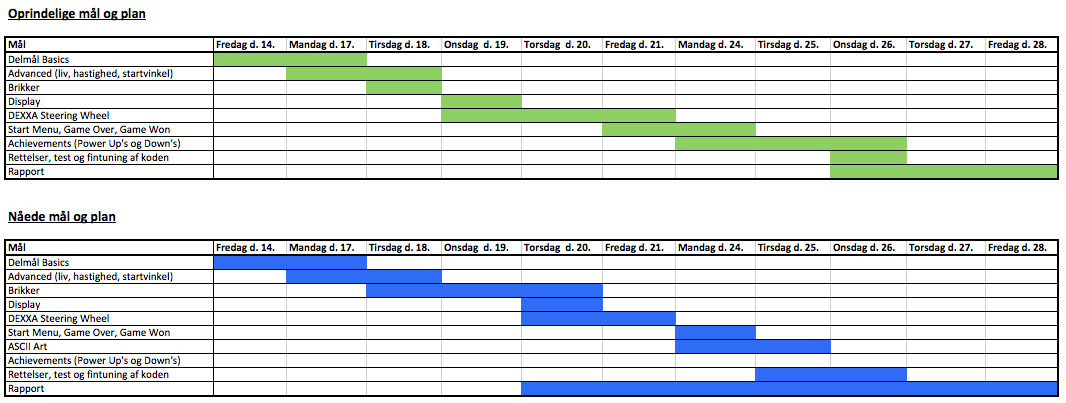
\includegraphics[width=\linewidth]{figs/Tidsplan2.png}
\caption{Øverst: Tidsplan over de forskellige delmål og hvornår de skulle være færdige. Nederst: Hvad vi rent faktisk lavede og hvornår}
\label{fig:tidsplan2}
\end{figure}

Forsinkelserne i projektet som kan ses på Figur \ref{fig:tidsplan2} skyldtes primært at vi, sammen med de avancerede delmål, valgte at gøre bolden større. Da vi skiftede til terminalen Putty i stedet for HyperTerminal og fik mulighed for at køre terminalen i fuldskærm valgte vi at lave bolden $4\times2$ karakterer. Dette gjorde, at bolden kunne ramme flere brikker af gangen, og briklogikken blev af den grund meget kompleks, se flowchartet på Figur \ref{fig:brickFlow} og  Appendix \nameref{reflexball}. En yderligere udfordring var, at bolden bevægede sig to karakterer af gangen i x-retningen på skærmen. Der kunne derfor komme en stor del af bolden ind i brikkerne, hvilket også vanskeliggjorde, at fastslå, hvordan brikken var blevet ramt af bolden. \\ 
En stor del af arbejdet med brikkerne bestod af debugging og rettelser i koden. For at teste briklogikken skrev vi tekst ud på skærmen der fortalte os hvordan vi havde ramt brikkerne, om flagene \texttt{dontDeflectX} og \texttt{dontDeflectY} var blevet sat og om det var detekteret at der var brikker ved siden af og over/under den ramte brik. På den måde kunne vi finde præcis de steder i koden hvor der var problemer med vores logik.\\

Hvis vi skulle have implementeret powerups i spillet kunne det være gjort ved at tjekke om en brik døde hver gang man ramte en brik. Hvis den gjorde det, kunne vi f.eks. lade de sidste tre bit af millis() bestemme om man fik en powerup. Hvis de sidste tre bit gav f.eks. 0 kunne man få en powerup. På den måde ville det være tilfældigt om man fik en powerup, man ville have 1/8 sandsynlighed for at det skete. \\

Den store udfordring med powerups er dog at implementere en masse forskellige sjove features de skulle have. En powerup kunne f.eks. give langsom hastighed, flere bolde, bredere striker, større/mindre bold, blinkende eller usynlig striker, blinkende level, flere brikker, mulighed for  at skyde eller mange andre ting. For at det skulle være en gennemført implementering af powerups skulle vi dog lave flere forskellige funktioner, og dette ville derfor blive et forholdsvis stort arbejde. Vi valgte derfor at fokusere på at lave et gennemført spil hvor detaljerne var i højsædet.\\

Vi forsøgte så vidt muligt at mindske antallet af globale variabler, da det hurtigt ville gøre koden meget uoverskuelig.\\
I de enkelte .c filer har vi forsøgt at bruge så få globale variabler defineret i andre filer som muligt, da det specielt ville gøre det hele meget uoverskueligt. \\
Det var dog svært helt at undgå globale variabler i takt med at koden blev mere og mere kompliceret. Specielt \nameref{reflexball}.c bruger en række globale variable. Vi mener dog ikke at de er brugt i unødvendigt, da de er nødvendige for at gemme information såsom brikken og strikerens position, antallet af liv brugeren har tilbage, tiden siden sidste iteration etc.
Vi har dog bestræbt os på at kalde de forskellige variabler så sigende navne som muligt, så der forhåbentligt opstår så lidt forvirring som muligt. 
		\newpage
\chapter{Konklusion}
Efter spillet et blevet designet, skrevet og uploadet til Zilog 6403 microcontrolleren, er alle spillets facetter blevet gennemtestet og fundet i overensstemmelse med det forventede resultat. Vi kan derfor konkludere at den skrevne kode implementerer spillet Reflex Ball på microcontrolleren og i hyperterminalen korrekt i forhold til vores specifikationskrav, bortset fra at vi aldrig nåede at implementere achievements-delen. Vi kan derudover også konkludere at alle spillets udvidelser virker som forventet uden fejl og mangler. \\


		
	%%%	Appendix %%%		
		\newpage\appendix
		\chapter{Intro-opgaver}

\begin{figure}[h!]
\centering
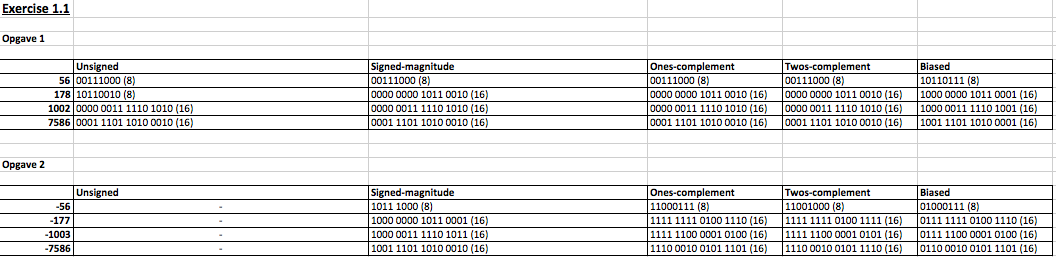
\includegraphics[scale=0.6]{figs/Ex1.1.png}
\caption{Exercise 1.1}
\label{fig:Ex1.1}
\end{figure}

\begin{figure}[h!]
\centering
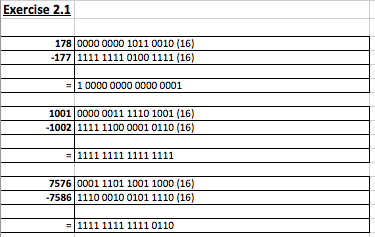
\includegraphics[scale=0.6]{figs/Ex2.1.png}
\caption{Exercise 2.1}
\label{fig:Ex2.1}
\end{figure}

\begin{figure}[h!]
\centering
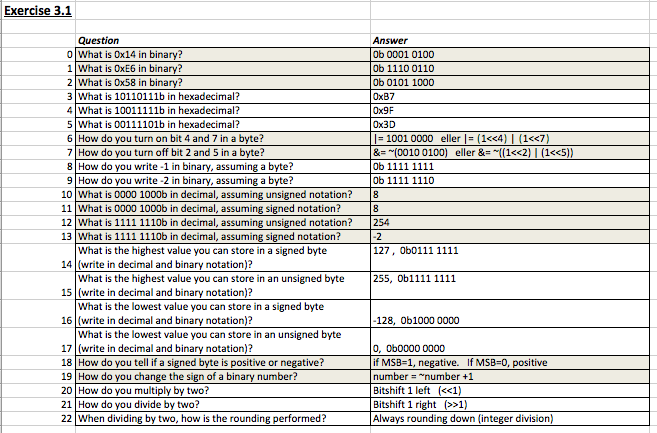
\includegraphics[scale=0.6]{figs/Ex3.1.png}
\caption{Exercise 3.1}
\label{fig:Ex3.1}
\end{figure}

\begin{figure}[h!]
\centering
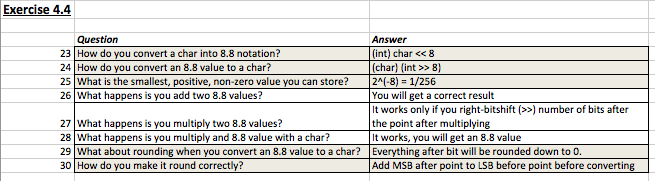
\includegraphics[scale=0.6]{figs/Ex4.4.png}
\caption{Exercise 4.4}
\label{fig:Ex4.4}
\end{figure}

		\chapter{Java kode}

\section{BackslashEscapes}
\label{BackslashEscapes}

\underline{BackslashEscapes.java}
\begin{lstlisting}[language=Java]

\end{lstlisting}
		\chapter{C kode}
\label{C kode}

Nedenfor ses hele vores færdige kode i alfabetisk rækkefølge. \\
Koden er skrevet i compileren Z8Encore! og implementeret på en Zilog 6403 mircocontroller. Da den er skrevet i C ville det dog ikke være så svært at porte den til anden hardware arkitektur. Man skulle således kunne ændre "Hardware Interface Layer" vist i figur \ref{fig:blockdiagram}.

\section{ansi}
\label{ansi}

\underline{ansi.h}
\begin{lstlisting}
#ifndef _ansi_h_
#define _ansi_h_

#define ESC 0x1B

#define UP		'A'
#define DOWN	'B'
#define FORWARD	'C'
#define BACK	'D'

// Public
void fgcolor(unsigned char foreground);
void bgcolor(unsigned char background);
void color(unsigned char foreground, unsigned char background);
void resetbgcolor();
void clrscr();
void clreol();
void gotoxy(unsigned char x, unsigned char y);
void underline(char on);
void blink(char on);
void reverse(char on);
unsigned char strlen(char* string);
void drawTopBot(unsigned char x, unsigned char y, unsigned char width, unsigned char left, unsigned char right, unsigned char side);
void drawSides(unsigned char x1, unsigned char y1, unsigned char x2, unsigned char y2, unsigned char side);
void saveCursor();
void getSavedCursor();
void moveCursor(char dir, unsigned char n);

// Private
void graphicCommand(char command);

#endif
\end{lstlisting}

\underline{ansi.c}
\begin{lstlisting}
#include <eZ8.h>             // special encore constants, macros and flash routines
#include <sio.h>             // special encore serial i/o routines
#include "ansi.h"

void fgcolor(unsigned char foreground) {
/*  Value      foreground     Value     foreground
    ------------------------------------------------
      0        Black            8       Dark Gray
      1        Red              9       Light Red
      2        Green           10       Light Green
      3        Brown           11       Yellow
      4        Blue            12       Light Blue
      5        Purple          13       Light Purple
      6        Cyan            14       Light Cyan
      7        Light Gray      15       White
*/
  int type = 22;             // normal text
	if (foreground > 7) {
	  type = 1;                // bold text
		foreground -= 8;
	}
  printf("%c[%d;%dm", ESC, type, foreground+30);
}

void bgcolor(unsigned char background) {
/* IMPORTANT:   When you first use this function you cannot get back to true white background in HyperTerminal.
   Why is that? Because ANSI does not support true white background (ANSI white is gray to most human eyes).
                The designers of HyperTerminal, however, preferred black text on white background, which is why
                the colors are initially like that, but when the background color is first changed there is no
 	              way comming back.
   Hint:        Use resetbgcolor(); clrscr(); to force HyperTerminal into gray text on black background.

    Value      Color      
    ------------------
      0        Black
      1        Red
      2        Green
      3        Brown
      4        Blue
      5        Purple
      6        Cyan
      7        Gray
*/
  printf("%c[%dm", ESC, background+40);
}

void color(unsigned char foreground, unsigned char background) { // combination of fgcolor() and bgcolor() - uses less bandwidth
  int type = 22;             // normal text
	if (foreground > 7) {
	  type = 1;                // bold text
		foreground -= 8;
	}
  printf("%c[%d;%d;%dm", ESC, type, foreground+30, background+40);
}

void resetbgcolor() {
  printf("%c[m", ESC); // Gray on black text, no underline, no blink, no reverse
}

void clrscr() {
	printf("%c[2J", ESC);	
}

void clreol() {
	printf("%c[K", ESC);	
}

void gotoxy(unsigned char x, unsigned char y) {
	printf("%c[%d;%dH", ESC, y, x);
}

void graphicCommand(char command) {
	printf("%c[%dm", ESC, command);
}

void underline(char on) {
	char command = 4;
	if (!on)
		command += 20;
	graphicCommand(command);
}

void blink(char on) {
	char command = 5;
	if (!on)
		command += 20;
	graphicCommand(command);	
}

void reverse(char on) {
	char command = 7;
	if (!on)
		command += 20;
	graphicCommand(command);
}

unsigned char strlen(char* string) {
	unsigned char length = 0;
	while(*string++ != '\0')
		length++;
	return length;
}

void drawTopBot(unsigned char x, unsigned char y, unsigned char width, unsigned char left, unsigned char right, unsigned char side) {
	int i;
	gotoxy(x,y);
	printf("%c",left);
	for (i=0;i<width;i++)
		printf("%c",side);
	printf("%c",right);
}

void drawSides(unsigned char x1, unsigned char y1, unsigned char x2, unsigned char y2, unsigned char side) {
	int i, j;
	for (i=y1+1;i<y2;i++) {
		gotoxy(x1,i);
		printf("%c",side);
		gotoxy(x2,i);
		printf("%c",side);
	}
}

void saveCursor() {
	printf("%c[s", ESC);
}

void getSavedCursor() {
	printf("%c[u", ESC);
}

void moveCursor(char dir, unsigned char n) {
	printf("%c[%d%c", ESC, n, dir);
}
\end{lstlisting}


\section{ascii}
\label{ascii}

\underline{ascii.h}
\begin{lstlisting}
#ifndef _ascii_h_
#define _ascii_h_

extern rom const char titleAscii1[11][127];
extern rom const char titleAscii2[11][127];
extern rom const char menuAscii[10][78];
extern rom const char easyAscii[8][24];
extern rom const char mediumAscii[6][38];
extern rom const char hardAscii[6][25];
extern rom const char chuckAscii1[9][66];
extern rom const char chuckAscii2[9][66];
extern rom const char wheelAscii[30][85];

extern rom const char gameOverAscii[8][75];
extern rom const char amigoAscii[5][61];
extern rom const char driveAscii[5][79];
extern rom const char havNoBallsAscii[5][135];
extern rom const char openEyesAscii[5][100];
extern rom const char patienceAscii[5][115];
extern rom const char notPassAscii[5][89];
extern rom const char thereIsNoBallAscii[5][127];
extern rom const char deadAscii[5][94];

extern rom const char ladyAscii[81][73];
extern rom const char chuckNorrisAscii[50][89];
extern rom const char congratulationsAscii[8][126];
extern rom const char nowTryAscii[5][108];
extern rom const char onlyChuckAscii[5][158];
extern rom const char chuckNorrisTextAscii[5][63];

#endif
\end{lstlisting}

\underline{ascii.c}
\begin{lstlisting}
#include "ascii.h"

rom const char titleAscii1[11][127] = {
	"                                                                               )                           (                ) ",
	"                                                                            ( /(         (                 )\\ )          ( /( ", 
	"                                                                           )\\) )(        ))\\       (      (()/(      (   )\\())",
	"                                                                          ((_) ()\\    ((()(_)(   ( )\\      /(_))     )\\ ((_)\\ ",
	"                                                                          (_()_((_)    )\\ __ )\\  )((_)    (__))     ((_)  ((_)",
	"                                                                          /\"      \\    (_)\"\"\\())((_) |    |\"  |     |\"  \\/\"  |",
	"__________        _____.__                __________        .__  .__     |:        |    /    \\_) ||  |    ||  |      \\   \\  / ",
	"\\______   \\ _____/ ____\\  |   ____ ___  __\\______   \\_____  |  | |  |    |_____/   )   /\' /\\  \\  |:  |    |:  |       \\\\  \\/  ",
	" |       _// __ \\   __\\|  | _/ __ \\\\  \\/  /|    |  _/\\__  \\ |  | |  |     //      /   //  __\'  \\  \\  |___  \\  |___    /   /   ",
	" |    |   \\  ___/|  |  |  |_\\  ___/ >    < |    |   \\ / __ \\|  |_|  |__  |:  __   \\  /   /  \\\\  \\( \\_|:  \\( \\_|:  \\  /   /    ",
	" |____|_  /\\___  >__|  |____/\\___  >__/\\_ \\|______  /(____  /____/____/  |__|  \\___)(___/    \\___)\\_______)\\_______)|___/     ",
};

rom const char titleAscii2[11][127] = {
	"                                                                               (                           )                ( ",
	"                                                                            ) \\)         )                 (/ (          ) \\) ",
	"                                                                           (/( ()        ((/       )      ))(\\)      )   (/)((",
	"                                                                          ))_( )(/    )))()_()   ) (/      \\)_((     (/ ))_(/ ",
	"                                                                          )_)(_))_(    (/ __ (/  ())_(    )__((     ))_(  ))_(",
	"                                                                          /\"      \\    )_(\"\"\\)(())_( |    |\"  |     |\"  \\/\"  |",
	"__________        _____.__                __________        .__  .__     |:        |    /    \\_( ||  |    ||  |      \\   \\  / ",
	"\\______   \\ _____/ ____\\  |   ____ ___  __\\______   \\_____  |  | |  |    |_____/   )   /\' /\\  \\  |:  |    |:  |       \\\\  \\/  ",
	" |       _// __ \\   __\\|  | _/ __ \\\\  \\/  /|    |  _/\\__  \\ |  | |  |     //      /   //  __\'  \\  \\  |___  \\  |___    /   /   ",
	" |    |   \\  ___/|  |  |  |_\\  ___/ >    < |    |   \\ / __ \\|  |_|  |__  |:  __   \\  /   /  \\\\  \\( \\_|:  \\( \\_|:  \\  /   /    ",
	" |____|_  /\\___  >__|  |____/\\___  >__/\\_ \\|______  /(____  /____/____/  |__|  \\___)(___/    \\___)\\_______)\\_______)|___/     ",
};

rom const char menuAscii[10][78] = {
	"                  /$$      /$$ /$$$$$$$$ /$$   /$$ /$$   /$$                 ",
	"                 | $$$    /$$$| $$_____/| $$$ | $$| $$  | $$                 ",
	"                 | $$$$  /$$$$| $$      | $$$$| $$| $$  | $$                 ",
	"                 | $$ $$/$$ $$| $$$$$   | $$ $$ $$| $$  | $$                 ",
	"                 | $$  $$$| $$| $$__/   | $$  $$$$| $$  | $$                 ",
	"                 | $$\\  $ | $$| $$      | $$\\  $$$| $$  | $$                 ",
	"                 | $$ \\/  | $$| $$$$$$$$| $$ \\  $$|  $$$$$$/                 ",
	"                 |__/     |__/|________/|__/  \\__/ \\______/                  ",
	" /$$$$$$$$$$$$$$$$$$$$$$$$$$$$$$$$$$$$$$$$$$$$$$$$$$$$$$$$$$$$$$$$$$$$$$$$$$$",
	"|___________________________________________________________________________/",
};

rom const char easyAscii[8][24] = {
	" ______                ",
 	"|  ____|               ",
 	"| |__   __ _ ___ _   _ ",
 	"|  __| / _` / __| | | |",
 	"| |___| (_| \\__ \\ |_| |",
 	"|______\\__,_|___/\\__, |",
    "                  __/ |",
    "                 |___/ ",
};

rom const char mediumAscii[6][38] = {
	" __  __          _ _                 ",
	"|  \\/  |        | (_)                ",
	"| \\  / | ___  __| |_ _   _ _ __ ___  ",
	"| |\\/| |/ _ \\/ _` | | | | | \'_ ` _ \\ ",
	"| |  | |  __/ (_| | | |_| | | | | | |",
	"|_|  |_|\\___|\\__,_|_|\\__,_|_| |_| |_|",
};

rom const char hardAscii[6][25] = {
	" _    _               _ ",
	"| |  | |             | |",
	"| |__| | __ _ _ __ __| |",
	"|  __  |/ _` | \'__/ _` |",
	"| |  | | (_| | | | (_| |",
	"|_|  |_|\\__,_|_|  \\__,_|",
};

rom const char chuckAscii1[9][66] = {
	"   (       )                          )                          ",
	"   )\\    ( /(                 )    ( /(     )    *               ",
	" (((_)   )\\())         (   ( /(   ((_))\\ ( /(  (  `     (        ",
	" )\\_____((_)\\    (     )\\ _)\\())  (_()(_))\\()) )\\))(    )\\    )  ",
	"((/ ____| |()(   )\\  (((_) (_)\\   | \\ | |(_)\\ ((_)()\\  ((_)  /(  ",
	" | |    | ((_) _ ((_))\\__| |((_)  |  \\| | ((_)(_()((_)__ _ _(_)) ",
	" | |    | \'_ \\| | | |/ __| |/ /   | . ` |/ _ \\| \'__| \'__| / __/( ",
	" | |____| | | | |_| | (__|   <    | |\\  | (_) | |  | |  | \\__ \\))",
	"  \\_____|_| |_|\\__,_|\\___|_|\\_\\   |_| \\_|\\___/|_|  |_|  |_|___/  ",
};

rom const char chuckAscii2[9][66] = {
	"   )       (                          (                          ",
	"   (/    ) \\)                 (    ) \\)     )   *                ",
	" )))_(   (\\)((         )   ) \\)   ))_((\\ ) \\)  )   `    )        ",
	" (/_____))_(/    )     (/ _(/)((  )_)()_((/)(( (/(()    (/    (  ",
	"))\\ ____| |)()   )/  )))_( )_(/   | \\ | |)_(/ ))_()(/  ))_(  \\)  ",
	" | |    | ))_( _ ))_((/__| |))_(  |  \\| | ))_()_)())_(__ _ _)_(( ",
	" | |    | \'_ \\| | | |/ __| |/ /   | . ` |/ _ \\| \'__| \'__| / __/) ",
	" | |____| | | | |_| | (__|   <    | |\\  | (_) | |  | |  | \\__ \\((",
	"  \\_____|_| |_|\\__,_|\\___|_|\\_\\   |_| \\_|\\___/|_|  |_|  |_|___/  ",
};

rom const char wheelAscii[30][85] = {
	"     Left   ____-------         ------____    Right                                 ",
	"        ___/                              \\___                                      ",
	"     __/           /////////\\\\\\\\\\\\\\\\          \\__                                   ",
	"    /         /////                 \\\\\\\\\\\\        \\                                 ",
	"  <-        ///    /////////\\\\\\\\\\\\\\\\    \\\\\\        ->                               ",
	"         //    ////                 \\\\\\\\    \\\\                                      ",
	"       //  ////                          \\\\    \\\\                                   ",
	"     //   //                               \\\\    \\\\                                 ",
	"    /    /                                   \\\\    \\                                ",
	"  //    /                                      \\    \\                               ",
	" /     /                                        \\    \\                              ",
	"|     /                 ________                \\     \\                             ",
	"|     \\\\_________///////        \\\\\\\\\\\\_________//      |                            ",
	"|                                                      |      //////\\\\\\\\\\\\          ",
	"|         |----------|            |----------|         |    //            \\\\        ",
	"|          \\   Enter (            )  Enter  /          |   /                \\      ^",
	"|           \\\\       (            )       //           |  |                  | Up  |",
	"|             \\\\_____|            |_____//             |  |                  |     |",
	"|     _________                          _________     |   \\\\              //      |",
	"|    |         \\\\\\                    ///         |    |     \\\\\\        ///         ",
	" \\   \\            \\\\                //           /    /         \\\\    //            ",
	" \\    \\             \\              /            /     /           |  |              ",
	"  \\    \\\\            \\            /            /     /            |  |             |",
	"   \\\\    \\            \\          /            /    //           __|  |__           |",
	"     \\    \\\\           |        |           //    /          ///        \\\\\\   Down |",
	"      \\\\    \\\\\\        |        |        ///    //          |              |       v",
	"        \\\\     \\\\\\\\____|        |____////    ///             \\____________/         ",
	"          \\\\\\                             ///                                       ",
	"             \\\\\\\\\\\\                 //////                                          ",
	"                   \\\\\\\\\\\\\\\\\\////////                                                ",
};

rom const char gameOverAscii[8][75] = {
	"      _____          __  __ ______    ______      ________ _____  _       ",
	"     / ____|   /\\   |  \\/  |  ____|  / __ \\ \\    / /  ____|  __ \\| |      ",
	"    | |  __   /  \\  | \\  / | |__    | |  | \\ \\  / /| |__  | |__) | |      ",
	"    | | |_ | / /\\ \\ | |\\/| |  __|   | |  | |\\ \\/ / |  __| |  _  /| |      ",
	"    | |__| |/ ____ \\| |  | | |____  | |__| | \\  /  | |____| | \\ \\|_|      ",
	"     \\_____/_/    \\_\\_|  |_|______|  \\____/   \\/   |______|_|  \\_(_)      ",
	" ________________________________________________________________________ ",
	"|________________________________________________________________________|",
};

rom const char amigoAscii[5][61] = {
	" ___          _   _         _                  _          _ ",
	"| _ ) __ _ __| | | |_  _ __| |__    __ _ _ __ (_)__ _ ___| |",
	"| _ \\/ _` / _` | | | || / _| / /_  / _` | \'  \\| / _` / _ \\_|",
	"|___/\\__,_\\__,_| |_|\\_,_\\__|_\\_( ) \\__,_|_|_|_|_\\__, \\___(_)",
	"                                |/               |___/      ",
};

rom const char driveAscii[5][79] = {
	"  ___                                                   _     _         _ ___ ",
	" / __|__ _ _ _    _  _ ___ _  _   _____ _____ _ _    __| |_ _(_)_ _____| |__ \\",
	"| (__/ _` | \' \\  | || / _ \\ || | / -_) V / -_) \' \\  / _` | \'_| \\ V / -_)_| /_/",
	" \\___\\__,_|_||_|  \\_, \\___/\\_,_| \\___|\\_/\\___|_||_| \\__,_|_| |_|\\_/\\___(_)(_) ",
	"                  |__/                                                        ",
};

rom const char havNoBallsAscii[5][135] = {
	" ___                _        _   _    _                                            _                              _          _ _    _ ",
	"| __|_ _____ _ _   (_)_ _   | |_| |_ (_)___  __ _ __ _ _ __  ___   _  _ ___ _  _  | |_  __ ___ _____   _ _  ___  | |__  __ _| | |__| |",
	"| _|\\ V / -_) \' \\  | | \' \\  |  _| \' \\| (_-< / _` / _` | \'  \\/ -_) | || / _ \\ || | | \' \\/ _` \\ V / -_) | \' \\/ _ \\ | \'_ \\/ _` | | (_-<_|",
	"|___|\\_/\\___|_||_| |_|_||_|  \\__|_||_|_/__/ \\__, \\__,_|_|_|_\\___|  \\_, \\___/\\_,_| |_||_\\__,_|\\_/\\___| |_||_\\___/ |_.__/\\__,_|_|_/__(_)",
	"                                             |___/                  |__/                                                              ",
};

rom const char openEyesAscii[5][100] = {
	"  ___                                                                      _     _   _           _ ",
	" / _ \\ _ __  ___ _ _    _  _ ___ _  _ _ _   ___ _  _ ___ ___  _ _  _____ _| |_  | |_(_)_ __  ___| |",
	"| (_) | \'_ \\/ -_) \' \\  | || / _ \\ || | \'_| / -_) || / -_|_-< | \' \\/ -_) \\ /  _| |  _| | \'  \\/ -_)_|",
	" \\___/| .__/\\___|_||_|  \\_, \\___/\\_,_|_|   \\___|\\_, \\___/__/ |_||_\\___/_\\_\\\\__|  \\__|_|_|_|_\\___(_)",
	"      |_|               |__/                    |__/                                               ",
};

rom const char patienceAscii[5][115] = {
	" ___      _   _                                                                         _                       _ ",
	"| _ \\__ _| |_(_)___ _ _  __ ___     _ __ _  _   _  _ ___ _  _ _ _  __ _   _ __  __ _ __| |__ ___ __ ____ _ _ _ | |",
	"|  _/ _` |  _| / -_) \' \\/ _/ -_)_  | \'  \\ || | | || / _ \\ || | \' \\/ _` | | \'_ \\/ _` / _` / _` \\ V  V / _` | \' \\|_|",
	"|_| \\__,_|\\__|_\\___|_||_\\__\\___( ) |_|_|_\\_, |  \\_, \\___/\\_,_|_||_\\__, | | .__/\\__,_\\__,_\\__,_|\\_/\\_/\\__,_|_||_(_)",
	"                               |/        |__/   |__/              |___/  |_|                                      ",
};

rom const char notPassAscii[5][89] = {
	" _____ _          _          _ _      _         _ _            _                      _ ",
	"|_   _| |_  ___  | |__  __ _| | |  __| |_  __ _| | |  _ _  ___| |_   _ __  __ _ _____| |",
	"  | | | \' \\/ -_) | \'_ \\/ _` | | | (_-< \' \\/ _` | | | | \' \\/ _ \\  _| | \'_ \\/ _` (_-<_-<_|",
	"  |_| |_||_\\___| |_.__/\\__,_|_|_| /__/_||_\\__,_|_|_| |_||_\\___/\\__| | .__/\\__,_/__/__(_)",
	"                                                                    |_|                 ",
};

rom const char thereIsNoBallAscii[5][127] = {
	" ___          _ _          _   _          _            _   _        _   _                  _                 _          _ _ _ ",
	"| _ \\___ __ _| (_)______  | |_| |_  ___  | |_ _ _ _  _| |_| |_     | |_| |_  ___ _ _ ___  (_)___  _ _  ___  | |__  __ _| | | |",
	"|   / -_) _` | | |_ / -_) |  _| \' \\/ -_) |  _| \'_| || |  _| \' \\ _  |  _| \' \\/ -_) \'_/ -_) | (_-< | \' \\/ _ \\ | \'_ \\/ _` | | |_|",
	"|_|_\\___\\__,_|_|_/__\\___|  \\__|_||_\\___|  \\__|_|  \\_,_|\\__|_||_( )  \\__|_||_\\___|_| \\___| |_/__/ |_||_\\___/ |_.__/\\__,_|_|_(_)",
	"                                                               |/                                                             ",
};

rom const char deadAscii[5][94] = {
	"__   __                            _             _                  __     _             _ _ ",
	"\\ \\ / /__ _  _   __ _ _ _ ___   __| |___ __ _ __| |    _ __ _  _   / _|_ _(_)___ _ _  __| | |",
	" \\ V / _ \\ || | / _` | \'_/ -_) / _` / -_) _` / _` |_  | \'  \\ || | |  _| \'_| / -_) \' \\/ _` |_|",
	"  |_|\\___/\\_,_| \\__,_|_| \\___| \\__,_\\___\\__,_\\__,_( ) |_|_|_\\_, | |_| |_| |_\\___|_||_\\__,_(_)",
	"                                                  |/        |__/                             ",
};

rom const char ladyAscii[81][73] = {
	"                            . ...                                       ",
	"                         .\'\'.\' .    \'.                                  ",
	"                    . \'\' \".\'.:I:.\'..  \'.                                ",
	"                  .\'.:.:..,,:II:\'.\'.\'.. \'.                              ",
	"                .\':.\'.:.:I:.:II:\'.\'.\'.\'.. \'.                            ",
	"              .\'.\'.\'.\'::.:.:.:I:\'.\'.\'.\'. .  \'                           ",
	"             ..\'.\'.\'.:.:I::.:II:.\'..\'.\'..    .                          ",
	"            ..\'.\'\':.:.::.:.::II::.\'.\'.\'.\'..   .                         ",
	"           ..\'.\'.\'.:.::. .:::II:..\'.\'.\'.\'.\'.   .                        ",
	"          .\':.\'\'.\':\'.\'.\'.:.:I:\'.\'.\'.\'.\'.. \'..  ..                       ",
	"          \':. \'.\':\'. ..:.::.::.:.\'..\'  \':.\'.\'.. ..                      ",
	"         .:.:.\':\'.   \'.:\':I:.:.. .\'.\'.  \': .\'.. . ..                    ",
	"         \'..:.:\'.   .:.II:.:..   . .:.\'. \'.. \'. .  ..                   ",
	"        .. :.:.\'.  .:.:I:.:. .  . ..:..:. :..\':. .  \'.                  ",
	"       .:. :.:.   .:.:I:.:. .    . ..:I::. :: ::  .. ..                 ",
	"       .. :\'.\'.:. .:.:I:\'.        ..:.:I:. :: ::.   . \'.                ",
	"       \'..:. .:.. .:II:\'         ,,;IIIH.  ::. \':.      .               ",
	"      .:.::\'.:::..:.AII;,      .::\",,  :I .::. \':.       .              ",
	"      :..:\'.:II:.:I:  ,,;\'   \' .;:FBT\"X:: ..:.. \':.    . .              ",
	"     .. :\':III:. :.:A\"PBF;.  . .P,IP;;\":: :I:..\'::. .    ..             ",
	"     . .:.:II: A.\'.\';,PP:\" .  . ..\'..\' .: :.::. \':...  . ..             ",
	"     . .: .:IIIH:.   \' \'.\' .  ... .    .:. :.:.. :...    .\'             ",
	"     . .I.::I:IIA.        ..   ...    ..::.\'.\'.\'.: ..  . .              ",
	"      .:II.\'.\':IA:.      ..    ..:.  . .:.: .\'\'.\'  ..  . .              ",
	"     ..::I:,\'.\'::A:.  . .:\'-, .-.:..  .:.::AA.. ..:.\' .. .              ",
	"      \':II:I:.  \':A:. ..:\'   \'\'.. . : ..:::AHI: ..:..\'.\'.               ",
	"     .\':III.::.   \'II:.:.,,;;;:::::\". .:::AHV:: .::\'\' ..                ",
	"     ..\":IIHI::. .  \"I:..\":;,,,,;;\". . .:AII:: :.:\'  . .                ",
	"     . . IIHHI:..\'.\'.\'V::. \":;;;\"   ...:AIIV:\'.:.\'  .. .                ",
	"      . . :IIHI:. .:.:.V:.   \' \' . ...:HI:\' .:: :. .  ..                ",
	"      . .  \':IHII:: ::.IA..      .. .A .,,:::\' .:.    .                 ",
	"      :.  ...\'I:I:.: .,AHHA, . .\'..AHIV::\' . .  :     ..                ",
	"      :. \'.::::II:.I:.HIHHIHHHHHIHHIHV:\'..:. .I.\':. ..  \'.              ",
	"   . . .. \'\':::I:\'.::IHHHHHHHHMHMHIHI. \'.\'.:IHI..  \'  \'  \'.             ",
	"    \':... .  \'\'\" .::\'.HMHI:HHHHMHHIHI. :IIHHII:. . . .    .             ",
	"     :.:.. . ..::.\' .IV\".:I:IIIHIHHIH. .:IHI::\'.\': \'..  .  .            ",
	"   . .:.:: .. ::\'.\'.\'..\':.::I:I:IHHHIA.\'.II.:...:\' .\' ... . \'..         ",
	"  \'..::::\' ...::\'.IIHII:: .:.:..:..:III:.\'::\' .\'    .    ..  . .        ",
	"  \'::.:\' .\'\'     .. :IIHI:.:.. ..: . .:I:\"\' ...:.:.  ..    .. ..        ",
	"     .:..::I:.  . . . .IHII:.:\'   .. ..\".::.:II:.:. .  ...   . ..       ",
	"  .. . .::.:.,,...-::II:.:\'    . ...... . .. .:II:.::  ...  .. ..       ",
	"   ..:.::.I .    . . .. .:. .... ...:.. . . ..:.::.   :..   . ..        ",
	"    .\'.::I:.      . .. ..:.... . ..... .. . ..::. .. .I:. ..\' .         ",
	"  .\'\':.: I.       . .. ..:.. .  . .. ..... .:. .:.. .:I.\'.\'\'..          ",
	"  . .:::I:.       . . .. .:. .    .. ..  . ... .:.\'.\'I\'  .  ...         ",
	"  . ::.:I:..     . . . ....:. . .   .... ..   .:...:.:.:. \'\'.\'\'         ",
	"  \'.\'::\'I:.       . .. ....:. .     .. . ..  ..\'  .\'.:..:..    \'        ",
	"        :. .     . .. .. .:.... .  .  .... ...   .  .:.:.:..    \'.      ",
	"        :.      .  . . .. .:.... . . ........       .:.:.::. .    .     ",
	"        :. .     . . . . .. .::..:  . ..:.. .        ::.:.:.. .    .    ",
	"        :.. .    . . .  . .. ..:.:  .. .. .:. ..     \':::.::.:. .   .   ",
	"        \':.. .  . . . .. .. ...::\' .. ..  . .:. .     V:I:::::.. .   :. ",
	"         ::. .  . .. .. ... .:.::  .. .  . .. .. .     VI:I:::::..   \'\'B",
	"          :.. .   . .. ..:.. ..I:... . .  . .. ... .    VII:I:I:::. .\'::",
	"          \':.. . . . .. ..:..:.:I:.:. .  . .. . .:. .    VHIII:I::.:..\':",
	"           ::..   . . .. ..:..:.HI:. .      . . .... .   :HHIHIII:I::..:",
	"           \':. .  . .. .. ..:.:.:HI:.    . . .. ..... .   HHHHIHII:I::.\'",
	"            :.. .  . . .. .:.:.:.HI:.      . . .. ... .   IHHHHIHHIHI:\' ",
	"             :..  .  . . .. ..:..IH:.     . . .. .. ,,, . \'HHHHHHHHI:\'  ",
	"             \':..   . . .. ..:.:.:HI..   .  . .. . :::::.  MIH:\"\"\"\'     ",
	"              :. . .  . .. ..::.:.VI:.     . . .. .:::\'::. HIH          ",
	"               :..  .  . .. .:.:.:.V:.    . . . ...::I\"A:. HHV          ",
	"                :. .  .  . .. ..:.:.V:.     . . ....::I::\'.HV:          ",
	"                 :. .  . . . .. .:..II:.  . . . ....\':::\' AV.\'          ",
	"                  :.. . . .. ... .:..VI:. . . .. .:. ..:.AV\'.           ",
	"                  \':.. . .  .. ..:.:.:HAI:.:...:.:.:.:.AII:.            ",
	"                   I:. .  .. ... .:.:.VHHII:..:.:..:A:\'.:..             ",
	"                   IA..  . . .. ..:.:.:VHHHHIHIHHIHI:\'.::.              ",
	"                   \'HA:.  . . .. ..:.:.:HHHIHIHHHIHI:..:.               ",
	"                    HIA: .  . . .. ...:.VHHHIHIIHI::.:...               ",
	"                    HIHI:. .  .. ... .::.HHHIIHIIHI:::..                ",
	"                    HII:.:.  .  .. ... .::VHHIHI:I::.:..                ",
	"                    AI:..:..  .  . .. ..:.VHIII:I::.:. .                ",
	"                   AI:. ..:..  .  . .. ..\' VHIII:I;... .                ",
	"                  AI:. .  .:.. .  .  . ...  VHIII::... .                ",
	"                .A:. .      :.. .  . .. .:.. VHII::..  .                ",
	"               A:. . .       ::. .. .. . .:.. \"VHI::.. .                ",
	"             .:.. .  .        :.. .:..... .::.. VHI:..                  ",
	"            ... . .  .     . . :.:. ..:. . .::.. VI:..  .               ",
	"           .. .. .  .    . . ...:... . .. . .:::. V:..  .               ",
	"          \'.. ..  .   .  .. ..:::.... .:. . ..::.. V..  .               ",
};

rom const char congratulationsAscii[8][126] = {
	"   _____                            _         _       _   _                  __     __          __          ______  _   _ _  ",
	"  / ____|                          | |       | |     | | (_)                 \\ \\   / /          \\ \\        / / __ \\| \\ | | | ",
	" | |     ___  _ __   __ _ _ __ __ _| |_ _   _| | __ _| |_ _  ___  _ __  ___   \\ \\_/ /__  _   _   \\ \\  /\\  / / |  | |  \\| | | ",
	" | |    / _ \\| \'_ \\ / _` | \'__/ _` | __| | | | |/ _` | __| |/ _ \\| \'_ \\/ __|   \\   / _ \\| | | |   \\ \\/  \\/ /| |  | | . ` | | ",
	" | |___| (_) | | | | (_| | | | (_| | |_| |_| | | (_| | |_| | (_) | | | \\__ \\    | | (_) | |_| |    \\  /\\  / | |__| | |\\  |_| ",
	"  \\_____\\___/|_| |_|\\__, |_|  \\__,_|\\__|\\__,_|_|\\__,_|\\__|_|\\___/|_| |_|___/    |_|\\___/ \\__,_|     \\/  \\/   \\____/|_| \\_(_) ",
	" __________________  __/ | _________________________________________________________________________________________________ ",
	"|__________________ |___/ __________________________________________________________________________________________________|",
};

rom const char nowTryAscii[5][108] = {
	" _  _              _               ___ _           _     _  _             _                    _       _ _ ",
	"| \\| |_____ __ __ | |_ _ _ _  _   / __| |_ _  _ __| |__ | \\| |___ _ _ _ _(_)___  _ __  ___  __| |___  | | |",
	"| .` / _ \\ V  V / |  _| \'_| || | | (__| \' \\ || / _| / / | .` / _ \\ \'_| \'_| (_-< | \'  \\/ _ \\/ _` / -_) |_|_|",
	"|_|\\_\\___/\\_/\\_/   \\__|_|  \\_, |  \\___|_||_\\_,_\\__|_\\_\\ |_|\\_\\___/_| |_| |_/__/ |_|_|_\\___/\\__,_\\___| (_|_)",
	"                           |__/                                                                            ",
};

rom const char chuckNorrisTextAscii[5][63] = {
	"   ________               __      _   __                _     ",
	"  / ____/ /_  __  _______/ /__   / | / /___  __________(_)____",
	" / /   / __ \\/ / / / ___/ //_/  /  |/ / __ \\/ ___/ ___/ / ___/",
	"/ /___/ / / / /_/ / /__/ ,<    / /|  / /_/ / /  / /  / (__  ) ",
	"\\____/_/ /_/\\__,_/\\___/_/|_|  /_/ |_/\\____/_/  /_/  /_/____/  ",
};

rom const char chuckNorrisAscii[50][89] = {
  "                                    MMMMMMMMMMM                                         ",
  "                                 MMMMMMMMMMMMMMMMM                                      ",
  "                             NMMMMMMMMMMMMMMMMMMMMMMMM                                  ",
  "                           MMMMMMMMMMMMMMMMMMMMMMMMMMMMMMM                              ",
  "                          MMMMMMMMMMMMMMMMMMMMMMMMMMMMMMMMMMMN                          ",
  "                          MMMMMMMMMMMMMMMMMMMMMMMMMMMMMMMMMMMMM                         ",
  "                         MMMMMMMMMMMMMMMMMMMMMMMMMMMMMMMMMMMMMMM                        ",
  "                         MMMMMMMMMMMMMMMMMMMMMMMMMMMMMMMMMMMMMMMD                       ",
  "                        DMMMMMMMMMMMMMMMMMMMMMMMMMMMMMMMMMMMMMMMM                       ",
  "                        MMMMMMMMMMMMMMMMMMMMMMMMMMMMMMMMMMMMMMMMM                       ",
  "                        MMMMMMMMMMMMMMMMMMMMMMMMMMMMMMMMMMMMMMMMM                       ",
  "                       MMMMMMMMMMMMMMMMMMMMMMMMMMMMMMMMMMMMMMMMMMM                      ",
  "                       MMMMMMMMMMMMMMMMMMMMMMMMMMMMMMMMMMMMMMMMMMM                      ",
  "                      MMMMMMMMMMMMMMMMMMMMMMMMMMMMMMMMMMMMMMMMMMMMN                     ",
  "                      MMMMMMMMMMMMMMMMMMMMMMMMMMMMMMMMMMMMMMMMMMMMMMMMMMMMMMMMN         ",
  "                     MMMMMMMMMMMMMMMMMMMMMMMMMMMMMMMMMMMMMMMMMMMMMMMMMMMMMMMMMMMMMN     ",
  "                     MMMMMMMMMMMMMMMMMMMMMMMMMMMMMMMMMMMMMMMMMMMMMMMMMMMMMMMMMMMMMMMN   ",
  "NM                  MMMMMMMMMMMMMMMMMMMMMMMMMMMMMMMMMMMMMMMMMMMMMMMMMMMMMMMMMMMMMMMMMM  ",
  "MMMMM              MMMMMMMMMMMMMMMMMMMMMMMMMMMMMMMMMMMMMMMMMMMMMMMMMMMMMMMMMMMMMMMMMMMM ",
  " MMMMMMMMMMMMMMMMMMMMMMMMMMMMMMMMMMMMMMMMMMMMMMMMMMMMMMMMMMMMMMMMMMMMMMMMMMMMMMMMMMMMMMM",
  "  MMMMMMMMMMMMMMMMMMMMMMMMMM8MMMMMMMMMIMMMMM8,. ...........OMMMMMMMMMMMMMMMMMMMMMMMMMMMM",
  "     MMMMMMMMMMMMMMMMMMMMMMM ..N. .....~MMMM...............:MMMMNMMMMMMMMMMMMMMMMMMMMMMM",
  "       NMMMMMMMMMMMMMMMMMMMMM.....:..DMMMMMNZ Z.... .......M$MMMMMMMMMMMMMMMMMMMMMMMMMMM",
  "           MMMMMMMMMMNMMMMMMM....... 7=MMMMMMO....Z .......MM7MMMMMMMMMMMMMMMMMMMMMMMMM ",
  "              MMMMMMMMMMMMMMMMM  Z...MMMZ .. .,M..,........MMMMMMMMMMMMMMMMMMMMMMMMMMMM ",
  "                  MMMMMM.......DOM ....N7..................MMMMMMMMMMMMMMMMMMMMMMMMMMM  ",
  "                     MMM....... M. ... .  ... ..............M...$MMMMMMMMMMMMMMMMMMMM   ",
  "                       ........... ........~. ..............M..=....+MMMMMMMMMMMMMM     ",
  "                       ......+.NMI~........ . ..............M.,.I...MMMMMMMMMMMMMMN     ",
  "                       ......$... ...... O..................,.....$MMMMMMMMMMMMN        ",
  "                       .....M.......... M M.. .............. 8  .OMMMMMMMMMMMN          ",
  "                        ..=7I,,.,,IMI...M.................. ..MMMMMMMMMMM               ",
  "                        ....DMMMMMMMMMMMMMMMO..............D...MMMMMMMMM                ",
  "                         .MMMMMMMMMMMMMMDDMM:,N..............DMMMMMMMMMMM               ",
  "                         NMMMMMNMM8 . .... ...,~............  MMMMMMMMM                 ",
  "                         MMMMM,:......::~..M8M8MM...............MMMMMM                  ",
  "                         MMMM ... . .........,MM..............MMMMMO$                   ",
  "                         MMMMM... =.=. .. . . MM ....... . ...MMMMMMM                   ",
  "                          NMMMMMMMMMM?  ..O.?NM7 ....... ......MMMMMM                   ",
  "                           NMMMMMMMMMMMMMMMMM........  $ . ...MMMNMMM                   ",
  "                            MMMMMMMMMMMMMMM.........,, ......MMMMMMMM                   ",
  "                             OMMMMMMMM8 , .. .. .,N.... ...:MMMMMMMMMMN                 ",
  "                              MMMMMMMM?N. ...~MD.:MNI8MMMMMMMMMMMMMMMMMN                ",
  "                         MMMMMMMMMMMMMMMMMMMMMMMMMMMMMMMMMMMMMMMMMMMMMMMMN              ",
  "                      NMMMMMMMMMMMMMMMMMMMMMMMMMMMMMMMMMMMMMMMMMMMMMMMMMMMN             ",
  "                     MMMMMMMMMMMMMMMMMMMMMMMMMMMMMMMMMMMMMMMMMMMMMMMMMMMMMMMMMMN        ",
  "                  MMMMMMMMMMMMMMMMMMMMMMMMMMMMMMMMMMMMMMMMMMMMMMMMMMMMMMMMMMMMMMMMM     ",
  "               MMMMMMMMMMMMMMMMMMMMMMMMMMMMMMMMMMMMMMMMMMMMMMMMMMMMMMMMMMMMMMMMMMMMM    ",
  "              NMMMMMMMMMMMMNMMMMMMMMMMMMMMMMMMMMMMMMMMMMMMMMMMMMMMMMMMMMMMMMMMMMMMMMMM  ",
  "             MMMMMMMMMMMMMMMMMMMMMMMMMMMMMMMMMMMMMMMMMMMMMMMMMMMMMMMMMMMMMMMMMMMMMMMMMM ",
};

rom const char onlyChuckAscii[5][158] = {
	"   ___       _         ___ _           _     _  _             _             _            ___ _           _     _  _             _                    _     _ ",
	"  / _ \\ _ _ | |_  _   / __| |_ _  _ __| |__ | \\| |___ _ _ _ _(_)___ __ __ _(_)_ _  ___  / __| |_ _  _ __| |__ | \\| |___ _ _ _ _(_)___  _ __  ___  __| |___| |",
	" | (_) | \' \\| | || | | (__| \' \\ || / _| / / | .` / _ \\ \'_| \'_| (_-< \\ V  V / | \' \\(_-< | (__| \' \\ || / _| / / | .` / _ \\ \'_| \'_| (_-< | \'  \\/ _ \\/ _` / -_)_|",
	"  \\___/|_||_|_|\\_, |  \\___|_||_\\_,_\\__|_\\_\\ |_|\\_\\___/_| |_| |_/__/  \\_/\\_/|_|_||_/__/  \\___|_||_\\_,_\\__|_\\_\\ |_|\\_\\___/_| |_| |_/__/ |_|_|_\\___/\\__,_\\___(_)",
	"               |__/                                                                                                                                          ",
};
\end{lstlisting}


\section{asciidisplay}
\label{asciidisplay}

\underline{asciidisplay.h}
\begin{lstlisting}
#ifndef _asciidisplay_h_
#define _asciidisplay_h_

extern unsigned char x1, y1, x2, y2;

// Public
unsigned char strlen_rom(rom const char *string);
void printAscii(rom const char *str, unsigned char size);
void printAsciiXY(rom const char *str, unsigned char size, unsigned char x, unsigned char y);
void initStartMenu(unsigned char x1, unsigned char y1, unsigned char x2, unsigned char y2);
unsigned char startMenu();
void printMenu();
unsigned char updateMenu();
void showWon();
void showGameOver();

// Private
void clearMenuBall(unsigned char x, unsigned char y);
void drawMenuBall(unsigned char x, unsigned char y);
void moveBall(char dir);
void calculateDifficulty();

#endif
\end{lstlisting}

\underline{asciidisplay.c}
\begin{lstlisting}
#include <eZ8.h>             // special encore constants, macros and flash routines
#include <sio.h>             // special encore serial i/o routines
#include "asciidisplay.h"
#include "ansi.h"
#include "LED.h"
#include "time.h"
#include "buttons.h"
#include "gameport.h"
#include "ascii.h"
#include "reflexball.h"

const unsigned char ballMenuYPos[4] = { 40, 48, 55, 64 };
const unsigned char ballXPos = 85;
unsigned char ballY, lastBallY;

unsigned char menuState;
unsigned long timer;
unsigned char oldButtonsWheel, oldButtonsBoard;

unsigned char xMin, yMin, xMax, yMax;

const char *startString = "Press any key to continue";

unsigned char strlen_rom(rom const char *string) {
	unsigned char length = 0;
	while ((char)*string++ != '\0')
		length++;
	return length;
}

void printAscii(rom const char *str, unsigned char size) {	
	unsigned char i;

	for (i=1;i<=size;i++) {
		getSavedCursor();
		moveCursor(DOWN,i);
		while ((char)*str != '\0')
			printf("%c",*str++);
		str++;		
	}
	getSavedCursor();
	moveCursor(DOWN,size);
	saveCursor();
}

void printAsciiXY(rom const char *str, unsigned char size, unsigned char x, unsigned char y) {
	unsigned char i, length = strlen_rom(str);	
	for (i=0;i<size;i++) {
		gotoxy(x,y+i);
		while ((char)*str != '\0')
			printf("%c",*str++);
		str++;
	}
	moveCursor(BACK,length);
}

void clearMenuBall(unsigned char x, unsigned char y) {
	gotoxy(x,y);
	printf("    ");
	gotoxy(x,y+1);
	printf("    ");
}

void drawMenuBall(unsigned char x, unsigned char y) {
	const unsigned char top = 238, bottom = 95, slash = '/', backSlash = '\\';

	clearMenuBall(ballXPos,lastBallY);

	lastBallY = y;

	gotoxy(x,y);
	printf("%c%c%c%c",slash,top,top,backSlash);
	gotoxy(x,y+1);
	printf("%c%c%c%c",backSlash,bottom,bottom,slash);
}

void moveBall(char dir) {	
	if (ballY + dir >= sizeof(ballMenuYPos) || ballY + dir < 0)
		return;

	ballY += dir;
	drawMenuBall(ballXPos,ballMenuYPos[ballY]);
}

void showWon() {
	const char* highscoreString = "Good try! But the highscore is still held by:";
	clrscr();
	if (divider == 1) { // Chuck Norris mode		
		printAsciiXY(chuckNorrisAscii[0],sizeof(chuckNorrisAscii)/sizeof(chuckNorrisAscii[0]),(xMin+xMax)/2-strlen_rom(chuckNorrisAscii[0])/2,(yMin+yMax)/2-(sizeof(chuckNorrisAscii)/sizeof(chuckNorrisAscii[0]))/2-10);
		moveCursor(DOWN,1);
		moveCursor(BACK,strlen_rom(onlyChuckAscii[0])/2-strlen_rom(chuckNorrisAscii[0])/2);
		saveCursor();
		printAscii(onlyChuckAscii[0],sizeof(onlyChuckAscii)/sizeof(onlyChuckAscii[0]));
	} else {
		gotoxy(0,0);
		saveCursor();
		printAscii(ladyAscii[0],sizeof(ladyAscii)/sizeof(ladyAscii[0]));

		gotoxy((xMin+xMax)/2-strlen_rom(congratulationsAscii[0])/2+strlen_rom(ladyAscii[0])/2,20);		
		saveCursor();
		printAscii(congratulationsAscii[0],sizeof(congratulationsAscii)/sizeof(congratulationsAscii[0]));
		moveCursor(DOWN,1);
		moveCursor(FORWARD,strlen_rom(congratulationsAscii[0])/2-strlen_rom(nowTryAscii[0])/2);
		saveCursor();
		printAscii(nowTryAscii[0],sizeof(nowTryAscii)/sizeof(nowTryAscii[0]));
		
		moveCursor(DOWN,10);
		moveCursor(FORWARD,strlen_rom(nowTryAscii[0])/2-strlen(highscoreString)/2);
		blink(1);
		printf("%s",highscoreString);
		blink(0);
		moveCursor(DOWN,1);
		moveCursor(BACK,strlen(highscoreString)+strlen_rom(chuckNorrisTextAscii[0])/2-strlen(highscoreString)/2);
		saveCursor();
		printAscii(chuckNorrisTextAscii[0],sizeof(chuckNorrisTextAscii)/sizeof(chuckNorrisTextAscii[0]));
	}

	while (!getGameportButtons() && !readButtons() && !kbhit()); // Wait for button press
}

void showGameOver() {
	clrscr();
	printAsciiXY(gameOverAscii[0],sizeof(gameOverAscii)/sizeof(gameOverAscii[0]),(xMin+xMax)/2-strlen_rom(gameOverAscii[0])/2,(yMin+yMax)/2-(sizeof(gameOverAscii)/sizeof(gameOverAscii[0]))/2-5);
	moveCursor(DOWN,1);
	
	switch (millis() & 0x7) { // Pseudo random number from 0-7
		case 0:
			if (strlen_rom(gameOverAscii[0]) > strlen_rom(amigoAscii[0]))
				moveCursor(FORWARD,strlen_rom(gameOverAscii[0])/2-strlen_rom(amigoAscii[0])/2);
			else
				moveCursor(BACK,strlen_rom(amigoAscii[0])/2-strlen_rom(gameOverAscii[0])/2);
			saveCursor();
			printAscii(amigoAscii[0],sizeof(amigoAscii)/sizeof(amigoAscii[0]));
			break;
		case 1:
			if (strlen_rom(gameOverAscii[0]) > strlen_rom(driveAscii[0]))
				moveCursor(FORWARD,strlen_rom(gameOverAscii[0])/2-strlen_rom(driveAscii[0])/2);	
			else
				moveCursor(BACK,strlen_rom(driveAscii[0])/2-strlen_rom(gameOverAscii[0])/2);
			saveCursor();
			printAscii(driveAscii[0],sizeof(driveAscii)/sizeof(driveAscii[0])); // Center text below "Game Over!"
			break;
		case 2:
			if (strlen_rom(gameOverAscii[0]) > strlen_rom(havNoBallsAscii[0]))
				moveCursor(FORWARD,strlen_rom(gameOverAscii[0])/2-strlen_rom(havNoBallsAscii[0])/2);	
			else
				moveCursor(BACK,strlen_rom(havNoBallsAscii[0])/2-strlen_rom(gameOverAscii[0])/2);
			saveCursor();
			printAscii(havNoBallsAscii[0],sizeof(havNoBallsAscii)/sizeof(havNoBallsAscii[0])); // Center text below "Game Over!"
			break;
		case 3:
			if (strlen_rom(gameOverAscii[0]) > strlen_rom(openEyesAscii[0]))
				moveCursor(FORWARD,strlen_rom(gameOverAscii[0])/2-strlen_rom(openEyesAscii[0])/2);
			else
				moveCursor(BACK,strlen_rom(openEyesAscii[0])/2-strlen_rom(gameOverAscii[0])/2);
			saveCursor();
			printAscii(openEyesAscii[0],sizeof(openEyesAscii)/sizeof(openEyesAscii[0])); // Center text below "Game Over!"
			break;
		case 4:
			if (strlen_rom(gameOverAscii[0]) > strlen_rom(patienceAscii[0]))
				moveCursor(FORWARD,strlen_rom(gameOverAscii[0])/2-strlen_rom(patienceAscii[0])/2);	
			else
				moveCursor(BACK,strlen_rom(patienceAscii[0])/2-strlen_rom(gameOverAscii[0])/2);
			saveCursor();
			printAscii(patienceAscii[0],sizeof(patienceAscii)/sizeof(patienceAscii[0])); // Center text below "Game Over!"
			break;
		case 5:
			if (strlen_rom(gameOverAscii[0]) > strlen_rom(notPassAscii[0]))
				moveCursor(FORWARD,strlen_rom(gameOverAscii[0])/2-strlen_rom(notPassAscii[0])/2);	
			else
				moveCursor(BACK,strlen_rom(notPassAscii[0])/2-strlen_rom(gameOverAscii[0])/2);
			saveCursor();
			printAscii(notPassAscii[0],sizeof(notPassAscii)/sizeof(notPassAscii[0])); // Center text below "Game Over!"
			break;
		case 6:
			if (strlen_rom(gameOverAscii[0]) > strlen_rom(thereIsNoBallAscii[0]))
				moveCursor(FORWARD,strlen_rom(gameOverAscii[0])/2-strlen_rom(thereIsNoBallAscii[0])/2);	
			else
				moveCursor(BACK,strlen_rom(thereIsNoBallAscii[0])/2-strlen_rom(gameOverAscii[0])/2);
			saveCursor();
			printAscii(thereIsNoBallAscii[0],sizeof(thereIsNoBallAscii)/sizeof(thereIsNoBallAscii[0])); // Center text below "Game Over!"
			break;
		case 7:
			if (strlen_rom(gameOverAscii[0]) > strlen_rom(deadAscii[0]))
				moveCursor(FORWARD,strlen_rom(gameOverAscii[0])/2-strlen_rom(deadAscii[0])/2);	
			else
				moveCursor(BACK,strlen_rom(deadAscii[0])/2-strlen_rom(gameOverAscii[0])/2);
			saveCursor();
			printAscii(deadAscii[0],sizeof(deadAscii)/sizeof(deadAscii[0])); // Center text below "Game Over!"
			break;
	}
	while (!getGameportButtons() && !readButtons() && !kbhit()); // Wait for button press
}

void initStartMenu(unsigned char newX1, unsigned char newY1, unsigned char newX2, unsigned char newY2) {
	xMin = newX1;
	yMin = newY1;
	xMax = newX2;
	yMax = newY2;
	
	blink(1);
	gotoxy((xMin+xMax)/2-strlen(startString)/2,(yMin+yMax)/2-10);
	printf("%s",startString);
	blink(0);	

	printAsciiXY(wheelAscii[0],sizeof(wheelAscii)/sizeof(wheelAscii[0]),(xMin+xMax)/2-strlen_rom(wheelAscii[0])/2,yMax-sizeof(wheelAscii)/sizeof(wheelAscii[0])-15);
	
	gotoxy((xMin+xMax)/2-strlen_rom(titleAscii1[0])/2,(yMin+yMax)/2-25);
	saveCursor();
	
	timer = 0;
}

unsigned char startMenu() {
	if (millis() - timer > 200) {
		timer = millis();		

		switch (menuState) {
			case 0:
				printAscii(titleAscii1[0],sizeof(titleAscii1)/sizeof(titleAscii1[0]));
				moveCursor(UP,sizeof(titleAscii1)/sizeof(titleAscii1[0]));
				saveCursor();
				menuState = 1;
				break;
			 case 1:
				printAscii(titleAscii2[0],sizeof(titleAscii2)/sizeof(titleAscii2[0]));
				moveCursor(UP,sizeof(titleAscii2)/sizeof(titleAscii2[0]));
				saveCursor();
				menuState = 0;
				break;
		}
	}

	if (getGameportButtons()) {
 		oldButtonsWheel = getGameportButtons(); // Update oldButtons value, so it doesn't skip the next menu
 	    return 1;
 	} else if (readButtons()) {
		oldButtonsWheel = readButtons(); // Update oldButtons value, so it doesn't skip the next menu
 	    return 1;
	} else if (kbhit())
		return 1;

	return 0;
}

void printMenu() {		
	printAsciiXY(menuAscii[0],sizeof(menuAscii)/sizeof(menuAscii[0]),(xMin+xMax)/2-strlen_rom(menuAscii[0])/2,(yMin+yMax)/2-15);

	moveCursor(FORWARD,strlen_rom(menuAscii[0])/2-strlen_rom(chuckAscii1[0])/2+10);
	moveCursor(DOWN,1);
	saveCursor();

	printAscii(easyAscii[0],sizeof(easyAscii)/sizeof(easyAscii[0]));
	printAscii(mediumAscii[0],sizeof(mediumAscii)/sizeof(mediumAscii[0]));
	moveCursor(DOWN,1);
	saveCursor();
	printAscii(hardAscii[0],sizeof(hardAscii)/sizeof(hardAscii[0]));
	moveCursor(DOWN,1);
	saveCursor();
	
	menuState = 0;
	timer = 0;

	ballY = lastBallY = 0;
	drawMenuBall(ballXPos,ballMenuYPos[ballY]);
}

unsigned char updateMenu() {
	int input;
	unsigned char buttons, buttonsClick;

	switch (menuState) {
		case 0:
			if (millis() - timer > 200) {
				timer = millis();
				printAscii(chuckAscii1[0],sizeof(chuckAscii1)/sizeof(chuckAscii1[0]));
				moveCursor(UP,sizeof(chuckAscii1)/sizeof(chuckAscii1[0]));
				saveCursor();
				menuState = 1;
			}
			break;
		 case 1:
			if (millis() - timer > 200) {
				timer = millis();
				printAscii(chuckAscii2[0],sizeof(chuckAscii2)/sizeof(chuckAscii2[0]));
				moveCursor(UP,sizeof(chuckAscii2)/sizeof(chuckAscii2[0]));
				saveCursor();
				menuState = 0;
			}
			break;
	}
	buttons = getGameportButtons();
	if (buttons != oldButtonsWheel) {
		buttonsClick = buttons & ~oldButtonsWheel; // Only look at the buttons that have changed
		oldButtonsWheel = buttons;

		if (buttonsClick & 0x1) // Gear forward
			moveBall(-1);
		else if (buttonsClick & 0x4) // Gear backward
			moveBall(1);
		else if (buttonsClick & 0xA) { // Either of the wheel buttons
			calculateDifficulty();
			return 1;
		}
	} else if (kbhit()) {
		input = getch();
		if (input == ' ') { // Space
			calculateDifficulty();
			return 1;
		} else if (input == 65) // Up
			moveBall(-1);
		else if (input == 66) // Down
			moveBall(1);
	} else {
		buttons = readButtons();
		if (buttons != oldButtonsBoard) {
			buttonsClick = buttons & ~oldButtonsBoard; // Only look at the buttons that have changed
			oldButtonsBoard = buttons;

			if (buttonsClick & 0x2) { // Center
				calculateDifficulty();
				return 1;
			} else if (buttonsClick & 0x4) // Left
				moveBall(-1);
			else if (buttonsClick & 0x1) // Right
				moveBall(1);
		}
	}
	return 0;
}

void calculateDifficulty() {	
	if (ballY == 0) { // Easy
		divider = 10;
		strikerWidth = 30;
	} else if (ballY == 1) { // Medium
		divider = 5;
		strikerWidth = 20;
	} else if (ballY == 2) { // Hard
		divider = 2;
		strikerWidth = 10;
	} else { // Chuck Norris
		divider = 1;
		strikerWidth = 4;
	}
}
\end{lstlisting}


\section{buttons}
\label{buttons}

\underline{buttons.h}
\begin{lstlisting}
#ifndef _buttons_h_
#define _buttons_h_

// Public
void initButtons();
unsigned char readButtons();
unsigned char readkey();

#endif
\end{lstlisting}

\underline{buttons.c}
\begin{lstlisting}
#include <eZ8.h>             // special encore constants, macros and flash routines
#include <sio.h>             // special encore serial i/o routines
#include "buttons.h"
#include "time.h"

void initButtons() {
	PDDD = (1 << 3);
	PFDD = (1 << 6) | (1 << 7);
}

unsigned char readButtons() {
	unsigned char inD, inF;
	inD = (~PDIN >> 3) & 0x1;
	inF = (~PFIN >> 6) & 0x3;
	return ((inF >> 1) | ((inF & 0x1) << 1) | (inD << 2));
}

unsigned char readkey() { // Read button with debounce
	unsigned char output = readButtons();
	delay_ms(50); // Wait 50ms
	output &= readButtons(); // Check if it is still high
	return output;
}
\end{lstlisting}


\section{charset}
\label{charset}

\underline{charset.h}
\begin{lstlisting}
/*************************************************
 *
 *  File Name: charset.h
 *
 *  Last modified:
 *  Michael Thomsen     21/03/2005
 *
 * 	Change log: none
 *************************************************/


/*** Supported ASCII characters ***

ASCII	CHAR	ASCII	CHAR	ASCII	CHAR	ASCII	CHAR	ASCII	CHAR	ASCII	CHAR
 0x20        0x30  0     0x40  @     0x50  P     0x60  `     0x70  p		
 0x21  !     0x31  1     0x41  A     0x51  Q     0x61  a     0x71  q		
 0x22  "     0x32  2     0x42  B     0x52  R     0x62  b     0x72  r
 0x23  #     0x33  3     0x43  C     0x53  S     0x63  c     0x73  s
 0x24  $     0x34  4     0x44  D     0x54  T     0x64  d     0x74  t
 0x25  %     0x35  5     0x45  E     0x55  U     0x65  e     0x75  u
 0x26  &     0x36  6     0x46  F     0x56  V     0x66  f     0x76  v
 0x27  '     0x37  7     0x47  G     0x57  W     0x67  g     0x77  w		
 0x28  (     0x38  8     0x48  H     0x58  X     0x68  h     0x78  x	
 0x29  )     0x39  9     0x49  I     0x59  Y     0x69  i     0x79  y
 0x2A  *     0x3A  :     0x4A  J     0x5A  Z     0x6A  j     0x7A  z
 0x2B  +     0x3B  ;     0x4B  K     0x5B  [     0x6B  k     0x7B  {
 0x2C  ,     0x3C  <     0x4C  L     0x5C  \     0x6C  l     0x7C  |
 0x2D  -     0x3D  =     0x4D  M     0x5D  ]     0x6D  m     0x7D  }
 0x2E  .     0x3E  >     0x4E  N     0x5E  ^     0x6E  n     0x7E  ~
 0x2F  /     0x3F  ?     0x4F  O     0x5F  _     0x6F  o
 
0x91 æ
0x9B ø
0x86 å
0x92 Æ
0x9D Ø
0x8F Å

Note: 
1. The ASCII character 0x20 is "SPACE" or a blank.
2. The ASCII character 0x7F(DEL) is not supported by the matrix below.

*/

#ifndef _CHARSET_H_
#define _CHARSET_H_

const unsigned char rom character_data[95+9][5] = {
  {0x00, 0x00, 0x00, 0x00, 0x00},
  {0x00, 0x5F, 0x5F, 0x00, 0x00},
  {0x00, 0x07, 0x00, 0x07, 0x00},
  {0x14, 0x7F, 0x14, 0x7F, 0x14},
  {0x24, 0x2A, 0x7F, 0x2A, 0x12},
  {0x23, 0x13, 0x08, 0x64, 0x62},
  {0x36, 0x49, 0x55, 0x22, 0x50},
  {0x00, 0x05, 0x03, 0x00, 0x00},
  {0x00, 0x1C, 0x22, 0x41, 0x00},
  {0x00, 0x41, 0x22, 0x1C, 0x00},
  {0x14, 0x08, 0x3E, 0x08, 0x14},
  {0x08, 0x08, 0x3E, 0x08, 0x08},
  {0x00, 0x50, 0x30, 0x00, 0x00},
  {0x08, 0x08, 0x08, 0x08, 0x08},
  {0x00, 0x60, 0x60, 0x00, 0x00},
  {0x20, 0x10, 0x08, 0x04, 0x02},
  {0x3E, 0x51, 0x49, 0x45, 0x3E},
  {0x00, 0x42, 0x7F, 0x40, 0x00},
  {0x42, 0x61, 0x51, 0x49, 0x46},
  {0x22, 0x49, 0x49, 0x49, 0x36},
  {0x18, 0x14, 0x12, 0x7F, 0x10},
  {0x2F, 0x49, 0x49, 0x49, 0x31},
  {0x3E, 0x49, 0x49, 0x49, 0x32},
  {0x03, 0x01, 0x71, 0x09, 0x07},
  {0x36, 0x49, 0x49, 0x49, 0x36},
  {0x26, 0x49, 0x49, 0x49, 0x3E},
  {0x00, 0x36, 0x36, 0x00, 0x00},
  {0x00, 0x56, 0x36, 0x00, 0x00},
  {0x08, 0x14, 0x22, 0x41, 0x00},
  {0x14, 0x14, 0x14, 0x14, 0x14},
  {0x00, 0x41, 0x22, 0x14, 0x08},
  {0x02, 0x01, 0x51, 0x09, 0x06},
  {0x32, 0x49, 0x79, 0x41, 0x3E},
  {0x7C, 0x0A, 0x09, 0x0A, 0x7C},
  {0x7F, 0x49, 0x49, 0x49, 0x36},
  {0x3E, 0x41, 0x41, 0x41, 0x22},
  {0x7F, 0x41, 0x41, 0x41, 0x3E},
  {0x7F, 0x49, 0x49, 0x49, 0x41},
  {0x7F, 0x09, 0x09, 0x09, 0x01},
  {0x3E, 0x41, 0x49, 0x49, 0x7A},
  {0x7F, 0x08, 0x08, 0x08, 0x7F},
  {0x00, 0x41, 0x7F, 0x41, 0x00},
  {0x30, 0x40, 0x40, 0x40, 0x3F},
  {0x7F, 0x08, 0x14, 0x22, 0x41},
  {0x7F, 0x40, 0x40, 0x40, 0x40},
  {0x7F, 0x02, 0x0C, 0x02, 0x7F},
  {0x7F, 0x02, 0x04, 0x08, 0x7F},
  {0x3E, 0x41, 0x41, 0x41, 0x3E},
  {0x7F, 0x09, 0x09, 0x09, 0x06},
  {0x3E, 0x41, 0x51, 0x21, 0x5E},
  {0x7F, 0x09, 0x09, 0x09, 0x76},
  {0x26, 0x49, 0x49, 0x49, 0x32},
  {0x01, 0x01, 0x7F, 0x01, 0x01},
  {0x3F, 0x40, 0x40, 0x40, 0x3F},
  {0x1F, 0x20, 0x40, 0x20, 0x1F},
  {0x3F, 0x40, 0x38, 0x40, 0x3F},
  {0x63, 0x14, 0x08, 0x14, 0x63},
  {0x03, 0x04, 0x78, 0x04, 0x03},
  {0x61, 0x51, 0x49, 0x45, 0x43},
  {0x7F, 0x41, 0x41, 0x00, 0x00},
  {0x02, 0x04, 0x08, 0x10, 0x20},
  {0x00, 0x41, 0x41, 0x7F, 0x00},
  {0x04, 0x02, 0x01, 0x02, 0x04},
  {0x40, 0x40, 0x40, 0x40, 0x40},
  {0x00, 0x01, 0x02, 0x04, 0x00},
  {0x20, 0x54, 0x54, 0x54, 0x78},
  {0x7F, 0x48, 0x44, 0x44, 0x38},
  {0x38, 0x44, 0x44, 0x44, 0x20},
  {0x38, 0x44, 0x44, 0x48, 0x7F},
  {0x38, 0x54, 0x54, 0x54, 0x18},
  {0x08, 0x7E, 0x09, 0x01, 0x02},
  {0x0C, 0x52, 0x52, 0x52, 0x3E},
  {0x7F, 0x08, 0x04, 0x04, 0x78},
  {0x00, 0x44, 0x7D, 0x40, 0x00},
  {0x20, 0x40, 0x44, 0x3D, 0x00},
  {0x7F, 0x10, 0x28, 0x44, 0x00},
  {0x00, 0x41, 0x7F, 0x40, 0x00},
  {0x7C, 0x04, 0x18, 0x04, 0x78},
  {0x7C, 0x08, 0x04, 0x04, 0x78},
  {0x38, 0x44, 0x44, 0x44, 0x38},
  {0x7C, 0x14, 0x14, 0x14, 0x08},
  {0x08, 0x14, 0x14, 0x18, 0x7C},
  {0x7C, 0x08, 0x04, 0x04, 0x08},
  {0x48, 0x54, 0x54, 0x54, 0x20},
  {0x04, 0x3F, 0x44, 0x40, 0x20},
  {0x3C, 0x40, 0x40, 0x20, 0x7C},
  {0x1C, 0x20, 0x40, 0x20, 0x1C},
  {0x3C, 0x40, 0x38, 0x40, 0x3C},
  {0x44, 0x28, 0x10, 0x28, 0x44},
  {0x0C, 0x50, 0x50, 0x50, 0x3C},
  {0x44, 0x64, 0x54, 0x4C, 0x44},
  {0x00, 0x08, 0x36, 0x41, 0x00},
  {0x00, 0x00, 0x7F, 0x00, 0x00},
  {0x00, 0x41, 0x36, 0x08, 0x00},
  {0x08, 0x04, 0x08, 0x10, 0x08},

  // Some special characters we created
  {0x24, 0x54, 0x78, 0x54, 0x58}, // æ
  {0x38, 0x64, 0x54, 0x4C, 0x38}, // ø
  {0x24, 0x54, 0x55, 0x54, 0x78}, // å
  {0x7E, 0x09, 0x7F, 0x49, 0x49}, // Æ
  {0x3C, 0x62, 0x5A, 0x46, 0x3C}, // Ø
  {0x78, 0x14, 0x15, 0x14, 0x78}, // Å
  {0X7F, 0x10, 0x20, 0x20, 0x1F}, // 
  {0x20, 0x46, 0x40, 0x46, 0x20}, // :)
  {0x1C, 0x3E, 0x7C, 0x3E, 0x1C} // <3
};

#endif /*! _ACHARSET_H_ */
\end{lstlisting}


\section{gameport}
\label{gameport}

\underline{gameport.h}
\begin{lstlisting}
#ifndef _gameport_h_
#define _gameport_h_

// Public
void initGameport();
unsigned char getGameportButtons();
char readSteeringWheel();

// Private
unsigned int readADC(unsigned char channel);

#endif
\end{lstlisting}

\underline{gameport.c}
\begin{lstlisting}
#include <eZ8.h>             // special encore constants, macros and flash routines
#include <sio.h>             // special encore serial i/o routines
#include "gameport.h"
#include "ansi.h"

unsigned int readADC(unsigned char channel) {
	unsigned char inHigh, inLow;
	unsigned int ADC_data;

	ADCCTL = 0x80 | 0x20 | (channel & 0x0F); // Enable ADC on the selected channel and use external voltage (3.3V) as VREF
	while (ADCCTL & 0x80); // Wait for conversion to be completed
	inHigh = ADCD_H; // ADC high byte
	inLow = ADCD_L; // ADC low low byte
	ADC_data = ((unsigned int)inHigh << 2)| inLow >> 6; // ADC output word

	return ADC_data;
}

void initGameport() {
	PBDD = (1 << 5) | (1 << 4) | (1 << 3) | (1 << 2); // Use PB2, PB3, PB4 and PB5 as digial inputs
	PBAF = (1 << 1) | (1 << 0); // Use PB0 and PB1 for ADC conversion
}

unsigned char getGameportButtons() {
	return (((~PBIN) & 0x3C) >> 2);
}

char readSteeringWheel() {
	int val = readADC(1);

	//gotoxy(50,10);
	//printf("Val: %04d",val);

	// The driving wheel is not linear therefor this table is needed
	if (val > 1000)
		return -6; // We will move it more aggressively to the side
	else if (val > 796)
		return -4;
	else if (val > 712)
		return -2;
	else if (val > 610)
		return -1;
	else if (val > 570)
		return 0;
	else if (val > 500)
		return 1;
	else if (val > 466)
		return 2;
	else if (val > 440)
		return 4;
	else
		return 6;
}
\end{lstlisting}

\section{LED}
\label{LED}

\underline{LED.h}
\begin{lstlisting}
#ifndef _led_h_
#define _led_h_

#define PRE1	(0 << 3);
#define PRE2	(1 << 3);
#define PRE4	(2 << 3);
#define PRE8	(3 << 3);
#define PRE16	(4 << 3);
#define PRE32	(5 << 3);
#define PRE64	(6 << 3);
#define PRE128	(7 << 3);

#define SCROLL_SPEED	5

// Public
void initLED(); // Initialize the LED display
void LEDsetString(char *string); // Used to scroll a string
void LEDRunOnce(char *firstString, char* secondString); // Used to sroll the first string once and then show the second string afterwards	

// Private
void clockLed(unsigned char digit);
unsigned char convertChar(char input);
void moveVideoBuffer();
void LEDupdate();
void timer2int();

#endif
\end{lstlisting}

\underline{LED.c}
\begin{lstlisting}
#include <eZ8.h>             // special encore constants, macros and flash routines
#include <sio.h>             // special encore serial i/o routines
#include "charset.h"
#include "LED.h"
#include "ansi.h"

unsigned char digit = 0, column = 0, delayCounter = 0, index = 0, stringLength = 0;
char videoBuffer[5][6];

volatile char runOnce, *pSecondString; // runOnce is used scroll a text only once, the pointer will point to the second string that is shown after the scroll is complete
char *pString; // Pointer to string in ram


void clockLed(unsigned char digit) {
	if (digit == 0) {
		PEOUT &= ~(1 << 7);
		PEOUT |= (1 << 7);
	}
	else if (digit == 1) {
		PGOUT |= (1 << 7);
		PGOUT &= ~(1 << 7);
	}
	else if (digit == 2) {
		PEOUT &= ~(1 << 5);
		PEOUT |= (1 << 5);
	}
	else if (digit == 3) {
		PEOUT &= ~(1 << 6);
		PEOUT |= (1 << 6);
	}
}

unsigned char convertChar(char input) { // Convert to some of our own characters
	unsigned char c;
	if (input == '')
		c = '~' + 1;
	else if (input == '\oe')
		c = '~' + 2;
	else if (input == 'å')
		c = '~' + 3;
	else if (input == 'Æ')
		c = '~' + 4;
	else if (input == 'Ø')
		c = '~' + 5;
	else if (input == 'Å')
		c = '~' + 6;
	else if (input == '')
		c = '~' + 7;
	else if (input == '') // Smiley
		c = '~' + 8;
	else if (input == '') // <3
		c = '~' + 9;
	else
		c = input;

	return c;
}

void LEDsetString(char *string) {
	unsigned char i, j;	

	DI(); // Disbable all interrupts

	runOnce = 0; // Reset flag
	stringLength = strlen(string); // Calculate length of string
	pString = string; // Set pointer to the start of the string

	for (i=0; i < 5; i++) {
		for (j=0;j<5;j++)			
			videoBuffer[i][j] = character_data[convertChar(*pString)-0x20][j];
		videoBuffer[i][5] = 0;

		pString++;
		if (*pString == '\0') {
			pString -= stringLength;
			break; // Break if we have reached the end of the string - this is due to the string being less than five characters wide
		}
	}
	for (i = stringLength; i < 4; i++) {
		for (j = 0; j < 5; j++)
			videoBuffer[i][j] = character_data[' '-0x20][j]; // Fill out the rest of the string with spaces if the string is less than five characters
	}

	digit = column = delayCounter = index = 0; // Reset all values used for multiplexing

	EI(); // Enable all interrupts
}

void LEDRunOnce(char *firstString, char* secondString) { // Used to sroll the first string once and then show the second string afterwards
	LEDsetString(firstString);
	runOnce = 1;
	pSecondString = secondString; // We will save the location of the second string
}

void moveVideoBuffer() {
	unsigned char i, j;

	for (i=0; i < 5; i++) {
		for (j=0;j<5;j++) {
			if (i < 4)
				videoBuffer[i][j] = videoBuffer[i+1][j]; // Shift all one to the left
			else
				videoBuffer[4][j] = character_data[convertChar(*pString)-0x20][j]; // Read the next character in the string
		}
	}
	pString++;
	if (*pString == '\0') { // Check if we have reached the end of the string
		if (runOnce) { // This wil actually abort when it loads the last character in the 5th digit, so you have to put a space in end of the sentence
			runOnce = 0;
			LEDsetString(pSecondString);
		} else
			pString -= stringLength;
	}
}

void LEDupdate() { // This function is called inside the interrupt
	PGOUT = (PGOUT & (1 << 7)) | *(&videoBuffer[0][0] + digit*6 + column + index);
	PEOUT |= 0x1F; // Set all cathodes high
	PEOUT &= ~(1 << (4-column)); // Set one cathodes low decided by column
	
	clockLed(digit);
	if (++digit == 4) {
		digit = 0;
		if (++column == 5) {
			column = 0;
			if (++delayCounter == SCROLL_SPEED && stringLength > 4) { // We don't have to scroll the text if there is less than five characters
				delayCounter = 0;				
				if (++index > 5) {
					index = 0;
					moveVideoBuffer();
				}
			}
		}
	}
}

#pragma interrupt
void timer2int() {
	LEDupdate();
}

void initLED() {
	unsigned char i;
	PEDD = 0; // All output
	PGDD = 0; // All output
	PEOUT = 0x1F; // Set clocks to low and cathodes to high
	PGOUT = 0; // Set all low

	for (i=0;i<4;i++) // Turn all off by default
		clockLed(i);

   	DI(); // Disable interrupt

	T2CTL = 0; // TEN - disable timer
	T2CTL |= PRE1; // PRES - Prescaler
	T2CTL |= (1 << 0); // TMODE - continuous mode

	T2H = 0;
	T2L = 1;
	
	T2RH = 9216 >> 8; // Interrupt every 500us
	T2RL = 9216 & 0xFF;

	SET_VECTOR(TIMER2, timer2int); // Enter the timer0int function at each interrupt
	
	// Set timer2 priority to low
	IRQ0ENH &= ~(1 << 7);
	IRQ0ENL |= (1 << 7);

	T2CTL |= (1 << 7); // TEN - enable timer

	EI(); // Enable interrupt
}
\end{lstlisting}


\section{levels}
\label{levels}

\underline{levels.h}
\begin{lstlisting}
#ifndef _levels_h_
#define _levels_h_

#include <eZ8.h>             // special encore constants, macros and flash routines
#include "reflexball.h"

// This array contains all the levels for the game
unsigned char rom levels[6][BRICK_TABLE_HEIGHT][BRICK_TABLE_WIDTH] = {
	{ // Bier
		{ 0, 0, 0, 0, 0, 0, 0, 0, 0, 0, 0, 0, 0, 0 },
		{ 0, 0, 0, 0, 0, 0, 0, 0, 0, 0, 0, 0, 0, 0 },
		{ 0, 0, 0, 0, 0, 0, 0, 0, 0, 0, 0, 0, 0, 0 },
		{ 0, 0, 0, 0, 0, 0, 0, 0, 0, 0, 0, 0, 0, 0 },
		{ 0, 0, 0, 0, 0, 0, 0, 0, 0, 0, 0, 0, 0, 0 },
		{ 0, 0, 0, 0, 0, 0, 0, 0, 0, 0, 0, 0, 0, 0 },
		{ 0, 0, 0, 0, 0, 0, 0, 0, 0, 0, 0, 0, 0, 0 },
		{ 1, 1, 1, 0, 1, 1, 1, 0, 1, 1, 1, 0, 1, 1 },
		{ 0, 3, 0, 2, 0, 3, 0, 2, 0, 3, 0, 2, 0, 3 },
		{ 1, 1, 1, 0, 1, 1, 1, 0, 1, 1, 1, 0, 1, 1 },
		{ 0, 3, 0, 2, 0, 3, 0, 2, 0, 3, 0, 2, 0, 3 },		
		{ 1, 1, 1, 0, 1, 1, 1, 0, 1, 1, 1, 0, 1, 1 },
		{ 0, 3, 0, 2, 0, 3, 0, 2, 0, 3, 0, 2, 0, 3 },
		{ 1, 1, 1, 0, 1, 1, 1, 0, 1, 1, 1, 0, 1, 1 },		
		{ 0, 0, 0, 0, 0, 0, 0, 0, 0, 0, 0, 0, 0, 0 },
		{ 0, 0, 0, 0, 0, 0, 0, 0, 0, 0, 0, 0, 0, 0 },
		{ 0, 0, 0, 0, 0, 0, 0, 0, 0, 0, 0, 0, 0, 0 },
		{ 0, 0, 0, 0, 0, 0, 0, 0, 0, 0, 0, 0, 0, 0 },
		{ 0, 0, 0, 0, 0, 0, 0, 0, 0, 0, 0, 0, 0, 0 },
		{ 0, 0, 0, 0, 0, 0, 0, 0, 0, 0, 0, 0, 0, 0 },
	},
	{ // Basic
		{ 0, 0, 0, 0, 0, 0, 0, 0, 0, 0, 0, 0, 0, 0 },
		{ 0, 0, 0, 0, 0, 0, 0, 0, 0, 0, 0, 0, 0, 0 },
		{ 0, 0, 0, 0, 0, 0, 0, 0, 0, 0, 0, 0, 0, 0 },
		{ 0, 0, 0, 0, 0, 0, 0, 0, 0, 0, 0, 0, 0, 0 },
		{ 0, 0, 0, 0, 0, 0, 0, 0, 0, 0, 0, 0, 0, 0 },
		{ 0, 0, 0, 0, 0, 0, 0, 0, 0, 0, 0, 0, 0, 0 },
		{ 0, 1, 1, 1, 1, 1, 1, 1, 1, 1, 1, 1, 1, 0 },
		{ 0, 1, 1, 1, 1, 1, 1, 1, 1, 1, 1, 1, 1, 0 },
		{ 0, 2, 2, 2, 2, 2, 2, 2, 2, 2, 2, 2, 2, 0 },
		{ 0, 3, 3, 3, 3, 3, 3, 3, 3, 3, 3, 3, 3, 0 },
		{ 0, 4, 4, 4, 4, 4, 4, 4, 4, 4, 4, 4, 4, 0 },
		{ 0, 0, 0, 0, 0, 0, 0, 0, 0, 0, 0, 0, 0, 0 },
		{ 0, 0, 0, 0, 0, 0, 0, 0, 0, 0, 0, 0, 0, 0 },
		{ 0, 0, 0, 0, 0, 0, 0, 0, 0, 0, 0, 0, 0, 0 },
		{ 0, 0, 0, 0, 0, 0, 0, 0, 0, 0, 0, 0, 0, 0 },
		{ 0, 0, 0, 0, 0, 0, 0, 0, 0, 0, 0, 0, 0, 0 },
		{ 0, 0, 0, 0, 0, 0, 0, 0, 0, 0, 0, 0, 0, 0 },
		{ 0, 0, 0, 0, 0, 0, 0, 0, 0, 0, 0, 0, 0, 0 },
		{ 0, 0, 0, 0, 0, 0, 0, 0, 0, 0, 0, 0, 0, 0 },
	},	
	{ // Cirkel
		{ 0, 0, 0, 0, 0, 1, 1, 1, 1, 0, 0, 0, 0, 0 },
		{ 0, 0, 0, 0, 1, 1, 0, 0, 1, 1, 0, 0, 0, 0 },
		{ 0, 0, 0, 1, 1, 0, 0, 0, 0, 1, 1, 0, 0, 0 },
		{ 0, 0, 1, 1, 0, 0, 2, 2, 0, 0, 1, 1, 0, 0 },
		{ 0, 0, 1, 0, 0, 2, 2, 2, 2, 0, 0, 1, 0, 0 },
		{ 0, 1, 0, 0, 2, 2, 0, 0, 2, 2, 0, 0, 1, 0 },
		{ 0, 1, 0, 2, 2, 0, 0, 0, 0, 2, 2, 0, 1, 0 },
		{ 0, 1, 0, 2, 0, 0, 4, 4, 0, 0, 2, 0, 1, 0 },
		{ 0, 1, 0, 2, 0, 0, 4, 4, 0, 0, 2, 0, 1, 0 },
		{ 0, 1, 0, 2, 2, 0, 0, 0, 0, 2, 2, 0, 1, 0 },
		{ 0, 1, 0, 0, 2, 2, 0, 0, 2, 2, 0, 0, 1, 0 },
		{ 0, 0, 1, 0, 0, 2, 2, 2, 2, 0, 0, 1, 0, 0 },
		{ 0, 0, 1, 1, 0, 0, 2, 2, 0, 0, 1, 1, 0, 0 },
		{ 0, 0, 0, 1, 1, 0, 0, 0, 0, 1, 1, 0, 0, 0 },
		{ 0, 0, 0, 0, 1, 1, 0, 0, 1, 1, 0, 0, 0, 0 },
		{ 0, 0, 0, 0, 0, 1, 1, 1, 1, 0, 0, 0, 0, 0 },
		{ 0, 0, 0, 0, 0, 0, 0, 0, 0, 0, 0, 0, 0, 0 },
		{ 0, 0, 0, 0, 0, 0, 0, 0, 0, 0, 0, 0, 0, 0 },
		{ 0, 0, 0, 0, 0, 0, 0, 0, 0, 0, 0, 0, 0, 0 },
	},
	{ // Blokke
		{ 0, 0, 0, 0, 0, 0, 0, 0, 0, 0, 0, 0, 0, 0 },
		{ 0, 0, 0, 0, 0, 0, 0, 0, 0, 0, 0, 0, 0, 0 },
		{ 0, 0, 0, 0, 0, 0, 0, 0, 0, 0, 0, 0, 0, 0 },
		{ 0, 0, 0, 0, 0, 0, 0, 0, 0, 0, 0, 0, 0, 0 },
		{ 0, 0, 0, 0, 0, 0, 0, 0, 0, 0, 0, 0, 0, 0 },
		{ 1, 1, 1, 1, 1, 1, 1, 1, 1, 1, 1, 1, 1, 1 },
		{ 1, 0, 2, 2, 0, 1, 1, 0, 2, 2, 0, 1, 1, 0 },
		{ 2, 0, 1, 1, 0, 2, 2, 0, 1, 1, 0, 2, 2, 0 },
		{ 1, 0, 2, 2, 0, 1, 1, 0, 2, 2, 0, 1, 1, 0 },
		{ 2, 0, 1, 1, 0, 2, 2, 0, 1, 1, 0, 2, 2, 0 },
		{ 1, 0, 2, 2, 0, 1, 1, 0, 2, 2, 0, 1, 1, 0 },
		{ 2, 0, 1, 1, 0, 2, 2, 0, 1, 1, 0, 2, 2, 0 },
		{ 1, 0, 2, 2, 0, 1, 1, 0, 2, 2, 0, 1, 1, 0 },
		{ 2, 0, 1, 1, 0, 2, 2, 0, 1, 1, 0, 2, 2, 0 },
		{ 1, 1, 1, 1, 1, 1, 1, 1, 1, 1, 1, 1, 1, 1 },
		{ 0, 0, 0, 0, 0, 0, 0, 0, 0, 0, 0, 0, 0, 0 },
		{ 0, 0, 0, 0, 0, 0, 0, 0, 0, 0, 0, 0, 0, 0 },
		{ 0, 0, 0, 0, 0, 0, 0, 0, 0, 0, 0, 0, 0, 0 },
		{ 0, 0, 0, 0, 0, 0, 0, 0, 0, 0, 0, 0, 0, 0 },
		{ 0, 0, 0, 0, 0, 0, 0, 0, 0, 0, 0, 0, 0, 0 },
	},
	{ // Batman
		{ 0, 0, 0, 0, 0, 0, 0, 0, 0, 0, 0, 0, 0, 0 },
		{ 0, 0, 0, 0, 0, 0, 0, 0, 0, 0, 0, 0, 0, 0 },
		{ 0, 0, 0, 0, 0, 0, 0, 0, 0, 0, 0, 0, 0, 0 },
		{ 1, 1, 0, 0, 0, 0, 0, 0, 0, 0, 0, 0, 1, 1 },
		{ 0, 1, 1, 0, 0, 0, 0, 0, 0, 0, 0, 1, 1, 0 },
		{ 0, 0, 1, 1, 0, 0, 0, 0, 0, 0, 1, 1, 0, 0 },
		{ 0, 0, 0, 1, 1, 0, 0, 0, 0, 1, 1, 0, 0, 0 },
		{ 0, 0, 0, 0, 1, 1, 0, 0, 1, 1, 0, 0, 0, 0 },
		{ 0, 2, 2, 0, 0, 1, 1, 1, 1, 0, 0, 2, 2, 0 },
		{ 0, 0, 2, 2, 0, 0, 1, 1, 0, 0, 2, 2, 0, 0 },
		{ 0, 0, 0, 2, 2, 0, 0, 0, 0, 2, 2, 0, 0, 0 },
		{ 0, 0, 0, 0, 2, 2, 0, 0, 2, 2, 0, 0, 0, 0 },
		{ 0, 0, 0, 0, 0, 2, 2, 2, 2, 0, 0, 0, 0, 0 },
		{ 0, 0, 1, 1, 0, 0, 2, 2, 0, 0, 1, 1, 0, 0 },
		{ 0, 0, 0, 1, 1, 0, 0, 0, 0, 1, 1, 0, 0, 0 },
		{ 0, 0, 0, 0, 1, 1, 0, 0, 1, 1, 0, 0, 0, 0 },
		{ 0, 0, 0, 0, 0, 1, 1, 1, 1, 0, 0, 0, 0, 0 },
		{ 0, 0, 0, 0, 0, 0, 1, 1, 0, 0, 0, 0, 0, 0 },
		{ 0, 0, 0, 0, 0, 0, 0, 0, 0, 0, 0, 0, 0, 0 },
		{ 0, 0, 0, 0, 0, 0, 0, 0, 0, 0, 0, 0, 0, 0 },
	},	
	{ // Usynlig
		{ 0, 0, 0, 0, 0, 0, 0, 0, 0, 0, 0, 0, 0, 0 },
		{ 0, 0, 0, 0, 0, 0, 0, 0, 0, 0, 0, 0, 0, 0 },
		{ 0, 0, 0, 0, 0, 0, 0, 0, 0, 0, 0, 0, 0, 0 },
		{ 0, 0, 0, 0, 0, 0, 0, 0, 0, 0, 0, 0, 0, 0 },
		{ 0, 0, 0, 0, 0, 0, 0, 0, 0, 0, 0, 0, 0, 0 },
		{ 1, 1, 1, 1, 1, 1, 1, 1, 1, 1, 1, 1, 1, 1 },
		{ 0, 0, 0, 0, 0, 0, 0, 0, 0, 0, 0, 0, 0, 0 },
		{ 0, 0, 0, 0, 0, 0, 0, 0, 0, 0, 0, 0, 0, 0 },
		{ 0, 0, 0, 0, 0, 0, 0, 0, 0, 0, 0, 0, 0, 0 },
		{ 0, 0, 0, 0, 0, 0, 0, 0, 0, 0, 0, 0, 0, 0 },
		{ 0, 0, 0, 0, 0, 0, 0, 0, 0, 0, 0, 0, 0, 0 },
		{ 0, 0, 0, 0, 0, 0, 0, 0, 0, 0, 0, 0, 0, 0 },
		{ 0, 0, 0, 0, 0, 0, 0, 0, 0, 0, 0, 0, 0, 0 },
		{ 0, 0, 0, 0, 0, 0, 0, 0, 0, 0, 0, 0, 0, 0 },
		{ 0, 0, 0, 0, 0, 0, 0, 0, 0, 0, 0, 0, 0, 0 },
		{ 5, 5, 5, 5, 5, 5, 5, 5, 5, 5, 5, 5, 5, 5 },
		{ 0, 0, 0, 0, 0, 0, 0, 0, 0, 0, 0, 0, 0, 0 },
		{ 0, 0, 0, 0, 0, 0, 0, 0, 0, 0, 0, 0, 0, 0 },
		{ 0, 0, 0, 0, 0, 0, 0, 0, 0, 0, 0, 0, 0, 0 },
	},
};

#endif
\end{lstlisting}


\section{lut}
\label{lut}

\underline{lut.h}
\begin{lstlisting}
// =====================================================================
//
//	Exported by Cearn's excellut v1.0
//	(comments, kudos, flames to daytshen@hotmail.com)
//
// =====================================================================

#ifndef LUT_H
#define LUT_H

// === LUT SIZES ===
#define SIN_SIZE 512

// === LUT DECLARATIONS ===
extern const signed short rom SIN[512];

#endif	// LUT_H
\end{lstlisting}

\underline{lut.c}
\begin{lstlisting}
// =====================================================================
//	  Look-Up Tables
//		SIN: sin(x*pi/256)
//
//	Exported by Cearn's excellut v1.0
//	(comments, kudos, flames to daytshen@hotmail.com)
//
// =====================================================================

#include "lut.h"
// -----------------------------------------------------------------------
// SIN: a 512 long LUT of 16bit values in 2.14 format
// sin(x*pi/256)
const signed short rom SIN[512]=
{
	0x0000,0x00C9,0x0192,0x025B,0x0324,0x03ED,0x04B5,0x057E,
	0x0646,0x070E,0x07D6,0x089D,0x0964,0x0A2B,0x0AF1,0x0BB7,
	0x0C7C,0x0D41,0x0E06,0x0ECA,0x0F8D,0x1050,0x1112,0x11D3,
	0x1294,0x1354,0x1413,0x14D2,0x1590,0x164C,0x1709,0x17C4,
	0x187E,0x1937,0x19EF,0x1AA7,0x1B5D,0x1C12,0x1CC6,0x1D79,
	0x1E2B,0x1EDC,0x1F8C,0x203A,0x20E7,0x2193,0x223D,0x22E7,
	0x238E,0x2435,0x24DA,0x257E,0x2620,0x26C1,0x2760,0x27FE,
	0x289A,0x2935,0x29CE,0x2A65,0x2AFB,0x2B8F,0x2C21,0x2CB2,

	0x2D41,0x2DCF,0x2E5A,0x2EE4,0x2F6C,0x2FF2,0x3076,0x30F9,
	0x3179,0x31F8,0x3274,0x32EF,0x3368,0x33DF,0x3453,0x34C6,
	0x3537,0x35A5,0x3612,0x367D,0x36E5,0x374B,0x37B0,0x3812,
	0x3871,0x38CF,0x392B,0x3984,0x39DB,0x3A30,0x3A82,0x3AD3,
	0x3B21,0x3B6D,0x3BB6,0x3BFD,0x3C42,0x3C85,0x3CC5,0x3D03,
	0x3D3F,0x3D78,0x3DAF,0x3DE3,0x3E15,0x3E45,0x3E72,0x3E9D,
	0x3EC5,0x3EEB,0x3F0F,0x3F30,0x3F4F,0x3F6B,0x3F85,0x3F9C,
	0x3FB1,0x3FC4,0x3FD4,0x3FE1,0x3FEC,0x3FF5,0x3FFB,0x3FFF,

	0x4000,0x3FFF,0x3FFB,0x3FF5,0x3FEC,0x3FE1,0x3FD4,0x3FC4,
	0x3FB1,0x3F9C,0x3F85,0x3F6B,0x3F4F,0x3F30,0x3F0F,0x3EEB,
	0x3EC5,0x3E9D,0x3E72,0x3E45,0x3E15,0x3DE3,0x3DAF,0x3D78,
	0x3D3F,0x3D03,0x3CC5,0x3C85,0x3C42,0x3BFD,0x3BB6,0x3B6D,
	0x3B21,0x3AD3,0x3A82,0x3A30,0x39DB,0x3984,0x392B,0x38CF,
	0x3871,0x3812,0x37B0,0x374B,0x36E5,0x367D,0x3612,0x35A5,
	0x3537,0x34C6,0x3453,0x33DF,0x3368,0x32EF,0x3274,0x31F8,
	0x3179,0x30F9,0x3076,0x2FF2,0x2F6C,0x2EE4,0x2E5A,0x2DCF,

	0x2D41,0x2CB2,0x2C21,0x2B8F,0x2AFB,0x2A65,0x29CE,0x2935,
	0x289A,0x27FE,0x2760,0x26C1,0x2620,0x257E,0x24DA,0x2435,
	0x238E,0x22E7,0x223D,0x2193,0x20E7,0x203A,0x1F8C,0x1EDC,
	0x1E2B,0x1D79,0x1CC6,0x1C12,0x1B5D,0x1AA7,0x19EF,0x1937,
	0x187E,0x17C4,0x1709,0x164C,0x1590,0x14D2,0x1413,0x1354,
	0x1294,0x11D3,0x1112,0x1050,0x0F8D,0x0ECA,0x0E06,0x0D41,
	0x0C7C,0x0BB7,0x0AF1,0x0A2B,0x0964,0x089D,0x07D6,0x070E,
	0x0646,0x057E,0x04B5,0x03ED,0x0324,0x025B,0x0192,0x00C9,

	0x0000,0xFF37,0xFE6E,0xFDA5,0xFCDC,0xFC13,0xFB4B,0xFA82,
	0xF9BA,0xF8F2,0xF82A,0xF763,0xF69C,0xF5D5,0xF50F,0xF449,
	0xF384,0xF2BF,0xF1FA,0xF136,0xF073,0xEFB0,0xEEEE,0xEE2D,
	0xED6C,0xECAC,0xEBED,0xEB2E,0xEA70,0xE9B4,0xE8F7,0xE83C,
	0xE782,0xE6C9,0xE611,0xE559,0xE4A3,0xE3EE,0xE33A,0xE287,
	0xE1D5,0xE124,0xE074,0xDFC6,0xDF19,0xDE6D,0xDDC3,0xDD19,
	0xDC72,0xDBCB,0xDB26,0xDA82,0xD9E0,0xD93F,0xD8A0,0xD802,
	0xD766,0xD6CB,0xD632,0xD59B,0xD505,0xD471,0xD3DF,0xD34E,

	0xD2BF,0xD231,0xD1A6,0xD11C,0xD094,0xD00E,0xCF8A,0xCF07,
	0xCE87,0xCE08,0xCD8C,0xCD11,0xCC98,0xCC21,0xCBAD,0xCB3A,
	0xCAC9,0xCA5B,0xC9EE,0xC983,0xC91B,0xC8B5,0xC850,0xC7EE,
	0xC78F,0xC731,0xC6D5,0xC67C,0xC625,0xC5D0,0xC57E,0xC52D,
	0xC4DF,0xC493,0xC44A,0xC403,0xC3BE,0xC37B,0xC33B,0xC2FD,
	0xC2C1,0xC288,0xC251,0xC21D,0xC1EB,0xC1BB,0xC18E,0xC163,
	0xC13B,0xC115,0xC0F1,0xC0D0,0xC0B1,0xC095,0xC07B,0xC064,
	0xC04F,0xC03C,0xC02C,0xC01F,0xC014,0xC00B,0xC005,0xC001,

	0xC000,0xC001,0xC005,0xC00B,0xC014,0xC01F,0xC02C,0xC03C,
	0xC04F,0xC064,0xC07B,0xC095,0xC0B1,0xC0D0,0xC0F1,0xC115,
	0xC13B,0xC163,0xC18E,0xC1BB,0xC1EB,0xC21D,0xC251,0xC288,
	0xC2C1,0xC2FD,0xC33B,0xC37B,0xC3BE,0xC403,0xC44A,0xC493,
	0xC4DF,0xC52D,0xC57E,0xC5D0,0xC625,0xC67C,0xC6D5,0xC731,
	0xC78F,0xC7EE,0xC850,0xC8B5,0xC91B,0xC983,0xC9EE,0xCA5B,
	0xCAC9,0xCB3A,0xCBAD,0xCC21,0xCC98,0xCD11,0xCD8C,0xCE08,
	0xCE87,0xCF07,0xCF8A,0xD00E,0xD094,0xD11C,0xD1A6,0xD231,

	0xD2BF,0xD34E,0xD3DF,0xD471,0xD505,0xD59B,0xD632,0xD6CB,
	0xD766,0xD802,0xD8A0,0xD93F,0xD9E0,0xDA82,0xDB26,0xDBCB,
	0xDC72,0xDD19,0xDDC3,0xDE6D,0xDF19,0xDFC6,0xE074,0xE124,
	0xE1D5,0xE287,0xE33A,0xE3EE,0xE4A3,0xE559,0xE611,0xE6C9,
	0xE782,0xE83C,0xE8F7,0xE9B4,0xEA70,0xEB2E,0xEBED,0xECAC,
	0xED6C,0xEE2D,0xEEEE,0xEFB0,0xF073,0xF136,0xF1FA,0xF2BF,
	0xF384,0xF449,0xF50F,0xF5D5,0xF69C,0xF763,0xF82A,0xF8F2,
	0xF9BA,0xFA82,0xFB4B,0xFC13,0xFCDC,0xFDA5,0xFE6E,0xFF37,
};
\end{lstlisting}


\section{main}
\label{main}

\underline{main.c}
\begin{lstlisting}
#include <eZ8.h>             // special encore constants, macros and flash routines
#include <sio.h>             // special encore serial i/o routines
#include "reflexball.h"
#include "ansi.h"
#include "LED.h"
#include "time.h"
#include "buttons.h"
#include "gameport.h"
#include "asciidisplay.h"
#include "ascii.h"

unsigned long wheelTimer;

void main() {
	int input;
	unsigned char buttons;
	char wheel;

	initTimers();
	initLED();
	initButtons();
	initGameport();
	init_uart(_UART0,_DEFFREQ,BAUD_115200);

	color(2,0); // Green forground, black background

Start:
	clrscr();

	LEDsetString("    ReflexBall RALLY!");

	initStartMenu(3,1,224,82); // x1, y1, x2, y2
	while(!startMenu()); // Wait for any key to be pressed
	clrscr();
	printMenu();
	while(!updateMenu()); // Wait until difficulty is choosen

	LEDsetString("    "); // Clear display
	initReflexBall(3,15,224,82,1); // x1, y1, x2, y2, style

	for(;;) {
		buttons = getGameportButtons();		
		
		if (buttons & 0xE) // Gear backward or button press
			startGame();
		else if (millis() - wheelTimer > 20) { // We have to limit the update rate or it will move to fast
			wheelTimer = millis();
			wheel = readSteeringWheel();
			if (wheel != 0)
				moveStriker(wheel);
		}
		else { // The driving wheel overrules the other controls
			buttons = readButtons();
			if (buttons) {
				if (buttons & 0x2) // Center
					startGame();
				else if (buttons & 0x4) // Left
					moveStriker(-1);
				else if (buttons & 0x1) // Right
					moveStriker(1);
			}
			else if (kbhit()) {
				input = getch();
				if (input == ' ') // Space
					startGame();
				else if (input == 68) // Left
					moveStriker(-2);
				else if (input == 67) // Right
					moveStriker(2);
			}
		}
		updateGame();
		if (restartGame)
			goto Start; // Goto back to the start of the game
	}
}
\end{lstlisting}

\section{math}
\label{math}

\underline{math.h}
\begin{lstlisting}
#ifndef _math_h_
#define _math_h_

#define FIX14_SHIFT 14

#define FIX14_MULT(a, b) ((a*b) >> FIX14_SHIFT)
#define FIX14_DIV(a, b) (a << FIX14_SHIFT / b)

typedef struct {
	long x,y;
} TVector;

// Public
long expand(long input);
void printNumber(long input, unsigned char decimalBits, unsigned char decimal);
void printFix(long input, unsigned char decimal);
long sin(int val);
long cos(int val);
void initVector(TVector* v, long x, long y);
void rotate(TVector* v, int val);
void printVector(TVector* v);

#endif
\end{lstlisting}

\underline{math.c}
\begin{lstlisting}
#include <eZ8.h>             // special encore constants, macros and flash routines
#include <sio.h>             // special encore serial i/o routines
#include "math.h"
#include "lut.h"

long expand(long input) {
	return input << 2; // Convert an 18.14 to 16.16
}

void printNumber(long input,  unsigned char decimalBits, unsigned char decimal) {
	int i;
	unsigned long pow = 10, mask = 0xFFFFFFFF, result, output;

	if ((input & 0x80000000) != 0) {
		printf("-");
		input = -input;
	}

	if (decimal > 5)
		decimal = 5;

	for (i=1;i<decimal;i++)
		pow *= 10;

	mask >>= (32 - decimalBits);
	result = pow * (unsigned long)(input & mask);
	output = result >> decimalBits;
	output += (result >> (decimalBits-1)) & 0x1; // Round correctly

	printf("%ld.%0*ld", input >> decimalBits, decimal, output);
}

void printFix(long input, unsigned char decimal) {
	printNumber(input,FIX14_SHIFT,decimal);
}

long sin(int val) {
	return SIN[val & 0x1FF];
}

long cos(int val) {
	return sin(val + 128);
}

void initVector(TVector* v, long x, long y) {
	v->x = x << FIX14_SHIFT;
	v->y = y << FIX14_SHIFT;
}

void rotate(TVector* v, int val) {
	long sinVal, cosVal, tempX;
 	sinVal = sin(val);
	cosVal = cos(val);
	tempX = v->x;

	v->x = FIX14_MULT(v->x,cosVal) - FIX14_MULT(v->y,sinVal);
	v->y = FIX14_MULT(tempX,sinVal) + FIX14_MULT(v->y,cosVal);
}

void printVector(TVector* v) {
	printf("(");
	printFix(v->x,4);
	printf(",");
	printFix(v->y,4);
	printf(")\n");
}
\end{lstlisting}


\section{reflexball}
\label{reflexball}

\underline{reflexball.h}
\begin{lstlisting}
#ifndef _reflexball_h_
#define _reflexball_h_

#include "ansi.h"
#include "math.h"

#define STRIKER_MAX_WIDTH	30 // This has to be even
#define STRIKER_MAX_ANGLE	64 // 360 deg = 512
#define NLIVES				3
#define DEFAULT_DIFFICULTY	40
#define UART_MAX_SPEED		20 // If it gets below this value, we will only draw it every second time or if it hits an object, this is because the UART can not send the characters fast enough
#define MAX_DIFFICULTY		10 // If speed gets under this value the UART can no longer keep up
#define BALL_WIDTH			4 // The modulus of this number should be even
#define BALL_HEIGHT			2

#define BRICK_TABLE_WIDTH	14
#define BRICK_TABLE_HEIGHT	20


typedef struct {
	long x, y; // (x,y) is in the top left corner - these use the 18.14 format
	unsigned char width, height;
	TVector vector;
} Ball;

typedef struct {
	unsigned char x, y, width;
} Striker;

typedef struct {
	unsigned char x, y; // (x,y) is in the top left corner
	unsigned char lives;
	unsigned char width, height;
} Brick;

extern unsigned char divider; // This is the difficulty set in the beginning
extern unsigned char strikerWidth; // This is the striker width determent from the selected difficulty
extern unsigned char restartGame; // True if the user have won the game

// Public
void initReflexBall(unsigned char newX1, unsigned char newY1, unsigned char newX2, unsigned char newY2, char style);
void startGame();
void stopGame();
void updateGame();
void moveStriker(char dir);

// Private
void printLevel();
void printLives();
void printScore();
void showScoreLED();
void scrollLiveInGameLED();
void scrollLevelUp();
void scrollAll();
void dead();
unsigned char getTerminalCoordinate(long input);
void gotoxyBall(long x, long y);
void clearBigBall(long x, long y);
void drawBigBall();
void drawBrick(Brick *brick);
void checkIteration(unsigned char x, unsigned char y);
void setBallPos(unsigned char x, unsigned char y);
void iterate();
void drawStriker();
void ballPosStriker();
void initStriker(unsigned char x, unsigned y, unsigned char width);
void initBricks(char clear);
void initBall();
void drawLevel();
void levelUp();

#endif
\end{lstlisting}

\underline{reflexball.c}
\begin{lstlisting}
#include <eZ8.h>             // special encore constants, macros and flash routines
#include <sio.h>             // special encore serial i/o routines
#include "reflexball.h"
#include "time.h"
#include "levels.h"
#include "LED.h"
#include "ascii.h"
#include "asciidisplay.h"

Ball ball;
Striker striker;
Brick bricks[BRICK_TABLE_HEIGHT][BRICK_TABLE_WIDTH];
unsigned char strikerAngle[STRIKER_MAX_WIDTH/2-1+BALL_WIDTH/2-1];
unsigned int bricksLives; // Stores the total number of lives of the bricks

unsigned long gameTimer;
unsigned char gameStarted = 0, alive;

unsigned char x1, y1, x2, y2;

unsigned int score, levelScore; // The total score and the score obtained in this level
unsigned char divider; // This is the difficulty set in the beginning
unsigned char strikerWidth; // This is the striker width determent from the selected difficulty

unsigned char lives, level;
volatile char runOnceBuf[50], ledBuf[50]; // We need this global buffer as the LED code creates a pointer to the memory location

char drawCounter = 0;
char drawCounterMax = 1;
char drawBallNow;

long lastX, lastY;

unsigned char restartGame; // True if the user have won the game

void printLevel() {
	gotoxy(x2-35,y2);
	printf("Level: %d", level+1);
}
void printLives() {
	gotoxy(x2-25,y2);
	printf("Lives: %d", lives);	
}
void printScore() {
	gotoxy(x2-15,y2);
	printf("Score: %04d$", score);
}

void showScoreLED() {
	sprintf(ledBuf,"%04d",score);
	LEDsetString(ledBuf);
}
void scrollLiveInGameLED() {
	sprintf(ledBuf,"%04d",score);
	sprintf(runOnceBuf,"%s$ Lives:%d %s ", ledBuf, lives, ledBuf); // We have to put a space behind as the LED routine aborts when it loaded the last character in the 5th digit
	
	LEDRunOnce(runOnceBuf,ledBuf);
}
void scrollLevelUp() {
	sprintf(ledBuf,"%04d", score);
	sprintf(runOnceBuf,"%s$ Level up! Level:%d Lives:%d %s ", ledBuf, level+1, lives, ledBuf); // We have to put a space behind as the LED routine aborts when it loaded the last character in the 5th digit
	
	LEDRunOnce(runOnceBuf,ledBuf);
}
void scrollAll() {
	sprintf(ledBuf,"%04d",score);
	sprintf(runOnceBuf,"%s$ Level:%d Lives:%d %s ", ledBuf, level+1, lives, ledBuf); // We have to put a space behind as the LED routine aborts when it loaded the last character in the 5th digit
	
	LEDRunOnce(runOnceBuf,ledBuf);
}

void dead() {
	if(--lives == 0) {
		delay_ms(1000); // Wait a bit before showing Game Over ASCII string
		sprintf(ledBuf,"%04d$ Game Over! Score:", score);
		LEDsetString(ledBuf);
		showGameOver();
		restartGame = 1;
		return;
	} else {
		scrollLiveInGameLED();
		printLives();
	}

	alive = 0;
	stopGame();	
}

unsigned char getTerminalCoordinate(long input) {
	unsigned char output = input >> FIX14_SHIFT;
	output += (input >> (FIX14_SHIFT-1)) & 0x1; // Round correctly
	return output;
}

void gotoxyBall(long x, long y) {
	gotoxy(getTerminalCoordinate(x),getTerminalCoordinate(y));
}

void clearBigBall(long x, long y) {
	gotoxyBall(x,y);
	printf("    ");
	gotoxyBall(x,y + ((long)1 << FIX14_SHIFT));
	printf("    ");
}

void drawBigBall() {
	const unsigned char top = 238, bottom = 95, slash = '/', backSlash = '\\';

	if ((++drawCounter != drawCounterMax && !drawBallNow) || !alive) // Check if we should skip the draweing in this iteration or if the game is not running
		return;
	drawCounter = 0;
	drawBallNow = 0;

	clearBigBall(lastX,lastY);

	lastX = ball.x;
	lastY = ball.y;

	gotoxyBall(ball.x,ball.y);
	printf("%c%c%c%c",slash,top,top,backSlash);
	gotoxyBall(ball.x,ball.y + ((long)1 << FIX14_SHIFT));
	printf("%c%c%c%c",backSlash,bottom,bottom,slash);
}

void drawBrick(Brick *brick) {
	unsigned char i, j, brickStyle;
	for (i=0;i<brick->height;i++) {
		gotoxy(brick->x,brick->y+i);
		for (j=0;j<brick->width;j++) {
			if (!brick->lives)
				brickStyle = ' ';
			else if (brick->lives == 1)
				brickStyle = 176;
			else if (brick->lives == 2)
				brickStyle = 177;
			else if (brick->lives == 3)
				brickStyle = 178;
			else if (brick->lives == 4)
				brickStyle = 219;
			else // Invisible
				brickStyle = ' ';
			printf("%c",brickStyle);			
		}
	}
}

void checkIteration(unsigned char x, unsigned char y) {
	unsigned char i, j, dontDeflectX = 0, dontDeflectY = 0, deflectedX = 0, deflectedY = 0;
	char distance; // Distance from center to ball position on striker
	int angle;

	if ((x > x1 && x+ball.width < x2 && y > y1 && y+ball.height-1 < y2-1) && gameStarted) {
		for (i=0;i<BRICK_TABLE_HEIGHT;i++) {
			for (j=0;j<BRICK_TABLE_WIDTH;j++) {
				if (!bricks[i][j].lives) // Skip if lives == 0
					continue;
	
				if (y-1 == bricks[i][j].y+bricks[i][j].height-1 || y+ball.height-1 == bricks[i][j].y-1 || x+ball.width-1 == bricks[i][j].x-1 || x-1 == bricks[i][j].x+bricks[i][j].width-1)
					drawBallNow = 1; // Make sure it draws the ball in this iteration

				// Check if the ball hit a brick
				if (y <= bricks[i][j].y+bricks[i][j].height-1 && y+ball.height-1 >= bricks[i][j].y && x+ball.width-1 >= bricks[i][j].x && x <= bricks[i][j].x+bricks[i][j].width-1) {
					score++;
					levelScore++;
					printScore();
					showScoreLED();
					
					// Check if the ball hit the top or the bottom of the brick
					if (y <= bricks[i][j].y+bricks[i][j].height-1 && y+ball.height-1 >= bricks[i][j].y) {												
			  		    if (!deflectedY) {
							if (x+ball.width-1 == bricks[i][j].x || x+ball.width-2 == bricks[i][j].x || x == bricks[i][j].x+bricks[i][j].width-1 || x == bricks[i][j].x+bricks[i][j].width-2) { // Left or right side
								if (y+ball.height-1 >= bricks[i][j].y && y <= bricks[i][j].y) { // Top left or right corner on brick
									if (i > 0 && bricks[i-1][j].lives) { // Make sure that there can actually be a brick above it
										dontDeflectY = 1; // Don't deflect it
										//gotoxy(x2-20,2);
										//printf("Alive above! %04d",dontCounter++);
									}
								}
								if (y <= bricks[i][j].y+bricks[i][j].height-1 && y+ball.height-1 >= bricks[i][j].y+bricks[i][j].height-1) { // Bottom left or right corner on brick
									if (i+1 < BRICK_TABLE_HEIGHT && bricks[i+1][j].lives) { // Make sure that there can actually be a brick underneath it
										dontDeflectY = 1; // Don't deflect it
										//gotoxy(x2-20,2);
										//printf("Alive below! %04d",dontCounter++);
									}
								}
							} else if (y >= bricks[i][j].y && y+ball.height-1 <= bricks[i][j].y+bricks[i][j].height-1) // Check if we hit the brick directly from the side
								dontDeflectY = 1;

							if (y+ball.height-1 >= bricks[i][j].y && y <= bricks[i][j].y) { // Top of brick
								if (ball.vector.y & 0x80000000) { // Negative
									dontDeflectY = 1; // Don't deflect it
									//gotoxy(x2-20,6);
									//printf("Top negative! %04d",dontCounter++);
								}
							}
							if (y <= bricks[i][j].y+bricks[i][j].height-1 && y+ball.height-1 >= bricks[i][j].y+bricks[i][j].height-1) { // Bottom of brick
								//gotoxy(x2-20,6);
								//printf("Bottom ");
								if (!(ball.vector.y & 0x80000000)) { // Positive
									dontDeflectY = 1; // Don't deflect it
									//printf("positive! %04d",dontCounter++);
								} /*else
									printf("negative! %04d",dontCounter++);*/
							}
							
							if (!dontDeflectY) {
								deflectedY = 1;
								ball.vector.y = -ball.vector.y;
								ball.y += 2*ball.vector.y;
							} /*else if (dontDeflectY) {
								gotoxy(10,4);
								printf("dontDeflectY: %d",dontCounter++);
							}*/
						}
					}
					// Check if the ball hit one of the sides of the brick
					if (x+ball.width-1 == bricks[i][j].x || x+ball.width-2 == bricks[i][j].x || x == bricks[i][j].x+bricks[i][j].width-1 || x == bricks[i][j].x+bricks[i][j].width-2) {						
						if (!deflectedX) {
							if ((y+ball.height-1 >= bricks[i][j].y && y <= bricks[i][j].y) || (y <= bricks[i][j].y+bricks[i][j].height-1 && y+ball.height-1 >= bricks[i][j].y+bricks[i][j].height-1)) { // Top or bottom of brick
								if (x+ball.width-1 == bricks[i][j].x || x+ball.width-2 == bricks[i][j].x) { // Top or bottom left side
									if (j > 0 && bricks[i][j-1].lives) { // Check if there is one alive to the left of the brick
										dontDeflectX = 1; // Don't deflect it
										//gotoxy(x2-20,4);
										//printf("Alive left! %04d",dontCounter++);
									}
								}
								if (x == bricks[i][j].x+bricks[i][j].width-1 || x == bricks[i][j].x+bricks[i][j].width-2) { // Top or bottom right side
									if (j+1 < BRICK_TABLE_WIDTH && bricks[i][j+1].lives) { // Check if there is one alive to the right of the brick
										dontDeflectX = 1; // Don't deflect it
										//gotoxy(x2-20,4);
										//printf("Alive right! %04d",dontCounter++);
									}
								}
							}
							
							if (x+ball.width-1 == bricks[i][j].x || x+ball.width-2 == bricks[i][j].x) { // Left side
								if (ball.vector.x & 0x80000000) { // Negative
									dontDeflectX = 1; // Don't deflect it
									//gotoxy(x2-20,8);
									//printf("Left negative! %04d",dontCounter++);
								}
							}
							if (x == bricks[i][j].x+bricks[i][j].width-1 || x == bricks[i][j].x+bricks[i][j].width-2) { // Right side
								if (!(ball.vector.x & 0x80000000)) { // Positive
									dontDeflectX = 1; // Don't deflect it
									//gotoxy(x2-20,8);
									//printf("Right positive! %04d",dontCounter++);
								}
							}
	
							if (y != bricks[i][j].y) { // It hasn't hit the brick directly from the side
								if (y < bricks[i][j].y) { // Top
									if (!(ball.vector.y & 0x80000000) && !(i > 0 && bricks[i-1][j].lives)) { // Check if it is positive and make sure there is no brick above
										dontDeflectX = 1; // Don't deflect it
										//gotoxy(x2-20,14);
										//printf("Top none above! %04d",dontCounter++);
									}
								} else { // Bottom
									if (ball.vector.y & 0x80000000 && !(i+1 < BRICK_TABLE_HEIGHT && bricks[i+1][j].lives)) { // Check if it is negative and make sure there is no brick below
										dontDeflectX = 1; // Don't deflect it
										//gotoxy(x2-20,14);
										//printf("Bottom none below! %04d",dontCounter++);
									}
								}								
							}

							if (!dontDeflectX) {
								deflectedX = 1;
								ball.vector.x = -ball.vector.x;
								ball.x += 2*ball.vector.x;
							} /*else if (dontDeflectX) {
								gotoxy(10,2);
								printf("dontDeflectX: %d",dontCounter++);
							}*/
						}						
					}
					bricks[i][j].lives--;
					bricksLives--;				
					drawBrick(&bricks[i][j]);
					if (!bricksLives) {
						levelUp();
						return;
					}
					ball.vector.x >>= 1; // We need to set this back again before rotating
					angle = (int)(millis() & 0x7) - 3; // Pseudo random number from -3 to 4
					//gotoxy(x1+10,y2-10);
					//printf("Angle: %02d", angle);
					rotate(&ball.vector, angle); // Slightly rotate the ball from -3 to 4, to make the game more exciting
					ball.vector.x <<= 1; // The x vector needs to be twice as large due to the y-axis being twice as high on the screen
				}			
			}
		}
	
		if (dontDeflectX && dontDeflectY) {
			//gotoxy(x2-20,12);
			//printf("CornerHit: %d",dontCounter++);
			ball.vector.y = -ball.vector.y;
			ball.y += 2*ball.vector.y;
			ball.vector.x = -ball.vector.x;
			ball.x += 2*ball.vector.x;
		}
	}
	else if (((y+ball.height-1 > striker.y) || (y+ball.height-1 == striker.y && (x+ball.width <= striker.x || x >= striker.x+striker.width))) && gameStarted) { // If you are below the striker then player must be dead	
		drawBallNow = 1;
		drawBigBall();
		dead();
		return;
	}
	else if (gameStarted) {
		if (x <= x1 || x+ball.width >= x2) {
			ball.vector.x = -ball.vector.x;
			ball.x += 2*ball.vector.x;
		}		
		if ((y <= y1) || (y+ball.height-1 == striker.y && x+ball.width > striker.x && x < striker.x+striker.width)) {
			if (y+ball.height-1 == striker.y) { // Check if we hit the striker
				printScore();
				showScoreLED();
	
				distance = x+ball.width-1 - striker.x;

				if (distance < striker.width/2-1+BALL_WIDTH/2-1) // The ball hit the left side
					angle = strikerAngle[(((striker.width/2-1)+(BALL_WIDTH/2-1))-1)-distance];
				else if (distance > striker.width/2+1+BALL_WIDTH/2-1) // The ball hit the right side
				 	angle = -(int)strikerAngle[distance-(((striker.width/2+1)+(BALL_WIDTH/2-1))+1)]; // IMPORTANT: remember to cast to int before the minus sign
				else
					angle = 0;

				if (angle != 0) {
					/*gotoxy(10,20);
					printf("                  ");
					gotoxy(10,20);
					printf("Rotating: %d", angle);*/


					ball.vector.x >>= 1; // We need to set this back again before rotating
					rotate(&ball.vector,angle);

					if (((ball.vector.y >> 12) & 0x7) == 0) { // Check if below 1/4 or approximately 15 degrees
						/*gotoxy(10,16);
						printf("BeforeY: ");
						printFix(ball.vector.y,4);*/
						ball.vector.y = 1 << 12; // 1/4
						/*printf(" AfterY: ");
						printFix(ball.vector.y,4);*/
				
						/*printf(" BeforeX: ");
						printFix(ball.vector.x,4);*/
						if (ball.vector.x & 0x80000000) // Negative
							ball.vector.x = -(long)15864; // -(cos(arcsin(1/4)) << 14)
						else
							ball.vector.x = 15864; // cos(arcsin(1/4)) << 14
						/*printf(" AfterX: ");
						printFix(ball.vector.x,4);*/
					}

					ball.vector.x <<= 1; // The x vector needs to be twice as large due to the y-axis being twice as high on the screen
				}
				/*gotoxy(10,10);
				printf("%02d %02d",distance,angle);*/
			}
			ball.vector.y = -ball.vector.y;
			ball.y += 2*ball.vector.y;
		}
	}

	if (x == x1+1 || x+ball.width == x2-1 || y == y1+1 || (y+ball.height-1 == striker.y-1 && x+ball.width > striker.x && x < striker.x+striker.width)) // Check if we are next to the sides, top or striker
		drawBallNow = 1; // If so then draw the ball in this iteration

	drawBigBall();	
}

void setBallPos(unsigned char x, unsigned char y) {
	ball.x = (long)x << FIX14_SHIFT;
	ball.y = (long)y << FIX14_SHIFT;
}

void iterate() {
	if (alive && gameStarted) {
		ball.x += ball.vector.x;
		ball.y += ball.vector.y;
	}
	checkIteration(getTerminalCoordinate(ball.x),getTerminalCoordinate(ball.y));
}

void drawStriker() {
	const unsigned char strikerStyle = 223;
	unsigned char i;
	gotoxy(striker.x,striker.y);
	if (divider == 1) // Blink striker if Chuck Norris mode is on
		blink(1);
	for (i=0;i<striker.width;i++)
		printf("%c",strikerStyle);
	if (divider == 1)
		blink(0);
}

void ballPosStriker() {
	setBallPos(striker.x+striker.width/2-ball.width/2,striker.y-ball.height);
	iterate();
	drawStriker(); // Redraw striker in case the ball clears part of the stikers
}

void moveStriker(char dir) { // Take care of moving the striker left or right
	char absDir = dir;
	if (!lives) // If no lives left then return
		return;	
	if (dir < 0)
		absDir = -dir;

	if ((int)striker.x + dir <= x1)
		striker.x = x1+1;
	else if (striker.x+striker.width-1 + dir >= x2)
		striker.x = x2-striker.width;
	else
		striker.x += dir;

	if (dir < 0) // Left
		gotoxy(striker.x+striker.width,striker.y);
	else // Right
		gotoxy(striker.x-dir,striker.y);

	for (; absDir > 0; absDir--)
		printf(" "); // Clear old char

	drawStriker();

	if (!gameStarted) {
		ballPosStriker();
		if (!alive)
			startGame();
	}
}

void initStriker(unsigned char x, unsigned y, unsigned char width) {
	unsigned char i, dAngle, strikerZones;

	if (width > STRIKER_MAX_WIDTH)
		width = STRIKER_MAX_WIDTH;

	strikerZones = width/2-1+BALL_WIDTH/2-1; // The striker is split up into zones to the left and right of the striker center

	striker.x = x - width/2;
	striker.y = y;
	striker.width = width;
	drawStriker();

	dAngle = STRIKER_MAX_ANGLE/strikerZones; // Delta angle between striker characters

	//gotoxy(10,8);
	for (i = 1; i <= strikerZones; i++) {
		strikerAngle[i-1] = dAngle*i; // Fill in the array - the longer distance from the center, the larger angle it will be reflected with
		//printf("%d ", strikerAngle[i-1]);
	}
}

void stopGame() {
	gameStarted = 0;
}

void initBricks(char clear) {
	unsigned char i, j;

	bricksLives = 0; // Reset

	for (i=0;i<BRICK_TABLE_HEIGHT;i++) {
		for (j=0;j<BRICK_TABLE_WIDTH;j++) {
			bricks[i][j].width = 14;
			bricks[i][j].height = 2;

			bricks[i][j].lives = levels[level][i][j];
			bricksLives += bricks[i][j].lives;
			bricks[i][j].x = x1+6 + (bricks[i][j].width+1)*j;
			bricks[i][j].y = y1+3 + (bricks[i][j].height+1)*i;
			if (bricks[i][j].lives || clear)
				drawBrick(&bricks[i][j]);
		}
	}
}

void startGame() {
	int startAngle;
	if (!alive) {
		alive = 1;
		if (lives == 0) {						
			score = 0;
			levelScore = 0;
			showScoreLED();
			initReflexBall(x1,y1,x2,y2,1);

			gameTimer = 0;
			printLives();
			printScore();			
			printLevel();
		}
		ballPosStriker();		
	} else if (!gameStarted) {
		initVector(&ball.vector,1,0);
		startAngle = (millis() & 0x7F) - 192; // Calculate a "random" angle from 0-127 (0-89.3 deg) and then subtract 192 (135 deg)

		//gotoxy(10,6);
		//printf("Start angle: %02d",(startAngle*360)/512);
		
		rotate(&ball.vector, startAngle);
		
		/*printf(" ");
		printFix(ball.vector.x,4);
		printf(" ");
		printFix(ball.vector.y,4);*/

		ball.vector.x <<= 1; // The x vector needs to be twice as large due to the y-axis being twice as high on the screen
		gameTimer = 0;
		gameStarted = 1;
		updateGame();
	}
}

void updateGame() {
	int speed = DEFAULT_DIFFICULTY-levelScore/divider; // Calculate teh speed using the score obtained in the current level and the divider set in the start up menu
	if (speed < MAX_DIFFICULTY || divider == 1) // Limit maximum speed and set maximum speed as default if Chuck Norris mode is enabled
		speed = MAX_DIFFICULTY;
		
	if (speed < UART_MAX_SPEED) // If it gets below this value, we will only draw it every second time or if it hits an object, this is because the UART can not send the characters fast enough
		drawCounterMax = 2;
	else
		drawCounterMax = 1;

	if (millis() - gameTimer > speed && gameStarted) {
		gameTimer = millis();
		iterate();
	}
}

void initBall() {
	setBallPos(striker.x+striker.width/2-2,striker.y-2); // Initialize the ball position to the striker position, as ballPosStriker will clear this
	ball.width = BALL_WIDTH; // This has to be even
	ball.height = BALL_HEIGHT;
	initVector(&ball.vector,0,0);
}
void drawLevel(char clear) {
	unsigned char i;

	gotoxy(striker.x,striker.y);
	for (i=0;i<striker.width;i++)
		printf(" "); // Clear old striker
	initStriker((x2-x1)/2+x1,y2-1,strikerWidth); // The width of the striker should always be even

	initBall(); // Initialize to striker position
	
	alive = 1;
	gameStarted = 0;
	ballPosStriker();

	printLives();
	printScore();	
	printLevel();

	gameTimer = 0;

	initBricks(clear);
}

void levelUp() {
	level++;	
	if (level >= sizeof(levels)/sizeof(levels[0])) { // Check if the user won the game
		showWon();
		if (divider != 1) { // If not in Chuck Norris mode, then the user wins the game
			restartGame = 1;
			return;
		}
		initReflexBall(x1,y1,x2,y2,1);
		return;
	}	
	lives += 2;
	
	levelScore = 0;
	scrollLevelUp();
	drawLevel(1);
}

void initReflexBall(unsigned char newX1, unsigned char newY1, unsigned char newX2, unsigned char newY2, char style) {
	unsigned char leftTop, rightTop, leftBot, rightBot, verSide, horSide, leftCross, rightCross;

	x1 = newX1;
	y1 = newY1;
	x2 = newX2;
	y2 = newY2;

	if (style) { // Bold
		leftTop = 201;
		rightTop = 187;
		leftBot = 200;
		rightBot = 188;
		verSide = 186;
		horSide = 205;
		leftCross = 185;
		rightCross = 204;
	} else { // Normal
		leftTop = 218;
		rightTop = 191;
		leftBot = 192;
		rightBot = 217;
		verSide = 179;
		horSide = 196;
		leftCross = 180;
		rightCross = 195;
	}

	lastX = (long)((x1+x2)/2) << FIX14_SHIFT; // Sets the last ball coordinates just above striker, so it clears the ball correctly the first time
	lastY = (long)(y2-1-BALL_HEIGHT) << FIX14_SHIFT;

	clrscr(); // Clear the screen
	
	// Put the title in the top of the screen - this is done when animateTitle() is called inside updateGame()
	printAsciiXY(titleAscii1[0],sizeof(titleAscii1)/sizeof(titleAscii1[0]),(x1+x2)/2-strlen_rom(titleAscii1[0])/2,y1/2-(sizeof(titleAscii1)/sizeof(titleAscii1[0]))/2);

	drawSides(x1,y1,x2,y2,verSide);	
	drawTopBot(x1,y1,x2-x1-1,leftTop,rightTop,horSide);
	
	restartGame = 0;
	level = 0;
	score = 0;
	levelScore = 0;
	lives = NLIVES;
	drawLevel(0);
	scrollAll();
}
\end{lstlisting}


\section{time}
\label{time}

\underline{time.h}
\begin{lstlisting}
#ifndef _time_h_
#define _time_h_

#define PRE1	(0 << 3);
#define PRE2	(1 << 3);
#define PRE4	(2 << 3);
#define PRE8	(3 << 3);
#define PRE16	(4 << 3);
#define PRE32	(5 << 3);
#define PRE64	(6 << 3);
#define PRE128	(7 << 3);

#define PRIORITY_TIMER0 (1 << 5)
#define PRIORITY_TIMER1 (1 << 6)
#define PRIORITY_TIMER2 (1 << 7)

// Public
void initTimers();
unsigned long millis();
void delay_ms(unsigned long time);

// Private
void timer1int();

#endif
\end{lstlisting}

\underline{time.c}
\begin{lstlisting}
#include <eZ8.h>             // special encore constants, macros and flash routines
#include <sio.h>             // special encore serial i/o routines
#include "time.h"
#include "ansi.h"

volatile unsigned long delayTimer, mscounter;

void initTimers() {
	DI(); // Disable interrupt

	T1CTL = 0; // TEN - disable timer
	T1CTL |= PRE1; // PRES - Prescaler
	T1CTL |= (1 << 0); // TMODE - continuous mode

	T1H = 0;
	T1L = 1;
	
	T1RH = 18432 >> 8; // Interrupt every 1ms
	T1RL = 18432 & 0xFF;

	SET_VECTOR(TIMER1, timer1int); // Enter the timer1int function at each interrupt
	
	// Set timer1 priority to high
	IRQ0ENH |= PRIORITY_TIMER1;
	IRQ0ENL |= PRIORITY_TIMER1;
	
	delayTimer = 0;
	mscounter = 0;

	T1CTL |= (1 << 7); // TEN - enable timer

	EI(); // Enable interrupt
}

unsigned long millis() {
	return mscounter;
}

void delay_ms(unsigned long time) { // This is not that acurate, but good enough for our needs
	delayTimer = time;
	while(delayTimer);
}

#pragma interrupt
void timer1int() {
	delayTimer--;
	mscounter++;
}
\end{lstlisting}

%%%%%%%%%%%%%%%%%%%%%%%%
%%% THE BIBLIOGRAPHY %%%
%%%%%%%%%%%%%%%%%%%%%%%%

		
	
		
\end{document}
